%**************************************%
%* Generated from MathBook XML source *%
%*    on 2017-05-23T15:38:09-07:00    *%
%*                                    *%
%*   http://mathbook.pugetsound.edu   *%
%*                                    *%
%**************************************%
\documentclass[10pt,]{book}
%% Custom Preamble Entries, early (use latex.preamble.early)
%% Inline math delimiters, \(, \), need to be robust
%% 2016-01-31:  latexrelease.sty  supersedes  fixltx2e.sty
%% If  latexrelease.sty  exists, bugfix is in kernel
%% If not, bugfix is in  fixltx2e.sty
%% See:  https://tug.org/TUGboat/tb36-3/tb114ltnews22.pdf
%% and read "Fewer fragile commands" in distribution's  latexchanges.pdf
\IfFileExists{latexrelease.sty}{}{\usepackage{fixltx2e}}
%% Text height identically 9 inches, text width varies on point size
%% See Bringhurst 2.1.1 on measure for recommendations
%% 75 characters per line (count spaces, punctuation) is target
%% which is the upper limit of Bringhurst's recommendations
%% Load geometry package to allow page margin adjustments
\usepackage{geometry}
\geometry{letterpaper,total={340pt,9.0in}}
%% Custom Page Layout Adjustments (use latex.geometry)
%% This LaTeX file may be compiled with pdflatex, xelatex, or lualatex
%% The following provides engine-specific capabilities
%% Generally, xelatex and lualatex will do better languages other than US English
%% You can pick from the conditional if you will only ever use one engine
\usepackage{ifthen}
\usepackage{ifxetex,ifluatex}
\ifthenelse{\boolean{xetex} \or \boolean{luatex}}{%
%% begin: xelatex and lualatex-specific configuration
%% fontspec package will make Latin Modern (lmodern) the default font
\ifxetex\usepackage{xltxtra}\fi
\usepackage{fontspec}
%% realscripts is the only part of xltxtra relevant to lualatex 
\ifluatex\usepackage{realscripts}\fi
%% 
%% Extensive support for other languages
\usepackage{polyglossia}
\setdefaultlanguage{english}
%% Magyar (Hungarian)
\setotherlanguage{magyar}
%% Spanish
\setotherlanguage{spanish}
%% Vietnamese
\setotherlanguage{vietnamese}
%% end: xelatex and lualatex-specific configuration
}{%
%% begin: pdflatex-specific configuration
%% translate common Unicode to their LaTeX equivalents
%% Also, fontenc with T1 makes CM-Super the default font
%% (\input{ix-utf8enc.dfu} from the "inputenx" package is possible addition (broken?)
\usepackage[T1]{fontenc}
\usepackage[utf8]{inputenc}
%% end: pdflatex-specific configuration
}
%% Monospace font: Inconsolata (zi4)
%% Sponsored by TUG: http://levien.com/type/myfonts/inconsolata.html
%% See package documentation for excellent instructions
%% One caveat, seem to need full file name to locate OTF files
%% Loads the "upquote" package as needed, so we don't have to
%% Upright quotes might come from the  textcomp  package, which we also use
%% We employ the shapely \ell to match Google Font version
%% pdflatex: "varqu" option produces best upright quotes
%% xelatex,lualatex: add StylisticSet 1 for shapely \ell
%% xelatex,lualatex: add StylisticSet 2 for plain zero
%% xelatex,lualatex: we add StylisticSet 3 for upright quotes
%% 
\ifthenelse{\boolean{xetex} \or \boolean{luatex}}{%
%% begin: xelatex and lualatex-specific monospace font
\usepackage{zi4}
\setmonofont[BoldFont=Inconsolatazi4-Bold.otf,StylisticSet={1,3}]{Inconsolatazi4-Regular.otf}
%% end: xelatex and lualatex-specific monospace font
}{%
%% begin: pdflatex-specific monospace font
\usepackage[varqu]{zi4}
%% end: pdflatex-specific monospace font
}
%% Symbols, align environment, bracket-matrix
\usepackage{amsmath}
\usepackage{amssymb}
%% allow page breaks within display mathematics anywhere
%% level 4 is maximally permissive
%% this is exactly the opposite of AMSmath package philosophy
%% there are per-display, and per-equation options to control this
%% split, aligned, gathered, and alignedat are not affected
\allowdisplaybreaks[4]
%% allow more columns to a matrix
%% can make this even bigger by overriding with  latex.preamble.late  processing option
\setcounter{MaxMatrixCols}{30}
%%
%% Color support, xcolor package
%% Always loaded.  Used for:
%% mdframed boxes, add/delete text, author tools
\PassOptionsToPackage{usenames,dvipsnames,svgnames,table}{xcolor}
\usepackage{xcolor}
%%
%% Semantic Macros
%% To preserve meaning in a LaTeX file
%% Only defined here if required in this document
%% Used for inline definitions of terms
\newcommand{\terminology}[1]{\textbf{#1}}
%% Subdivision Numbering, Chapters, Sections, Subsections, etc
%% Subdivision numbers may be turned off at some level ("depth")
%% A section *always* has depth 1, contrary to us counting from the document root
%% The latex default is 3.  If a larger number is present here, then
%% removing this command may make some cross-references ambiguous
%% The precursor variable $numbering-maxlevel is checked for consistency in the common XSL file
\setcounter{secnumdepth}{3}
%% mdframed environments use a tikz frame method
\usepackage{tikz}%% Environments with amsthm package
%% Theorem-like environments in "plain" style, with or without proof
\usepackage{amsthm}
\theoremstyle{plain}
%% Numbering for Theorems, Conjectures, Examples, Figures, etc
%% Controlled by  numbering.theorems.level  processing parameter
%% Always need a theorem environment to set base numbering scheme
%% even if document has no theorems (but has other environments)
\newtheorem{theorem}{Theorem}[chapter]
%% Only variants actually used in document appear here
%% Style is like a theorem, and for statements without proofs
%% Numbering: all theorem-like numbered consecutively
%% i.e. Corollary 4.3 follows Theorem 4.2
%% Remark-like environments, normal text
%% Numbering is in sync with theorems, etc
\theoremstyle{definition}
\newtheorem{remark}[theorem]{Remark}
%% Example-like environments, normal text
%% Numbering is in sync with theorems, etc
\theoremstyle{definition}
\newtheorem{example}[theorem]{Example}
%% Package for breakable highlight boxes
\usepackage[framemethod=tikz]{mdframed}
%% begin: assemblage
%% minimally structured content, high visibility presentation
%% environments (untitled, titled), with style
\newenvironment{assemblage-untitled}{\mdfsetup{%
roundcorner=2ex, backgroundcolor=blue!5,linecolor=blue!75!black,}%
\begin{mdframed}}{\end{mdframed}}
\newenvironment{assemblage}[1]{\mdfsetup{frametitle={\colorbox{blue!20}{\space#1\space}},%
frametitlealignment={\hspace*{1ex}}, frametitleaboveskip=-1.5ex, frametitlebelowskip=0pt,%
roundcorner=2ex, backgroundcolor=blue!5,linecolor=blue!75!black,}%
\begin{mdframed}}{\end{mdframed}}
%% end: assemblage
%% Miscellaneous environments, normal text
%% Numbering for inline exercises and lists is in sync with theorems, etc
\theoremstyle{definition}
\newtheorem{exercise}[theorem]{Exercise}
%% Localize LaTeX supplied names (possibly none)
\renewcommand*{\chaptername}{Chapter}
%% Equation Numbering
%% Controlled by  numbering.equations.level  processing parameter
\numberwithin{equation}{part}
%% For improved tables
\usepackage{array}
%% Some extra height on each row is desirable, especially with horizontal rules
%% Increment determined experimentally
\setlength{\extrarowheight}{0.2ex}
%% Define variable thickness horizontal rules, full and partial
%% Thicknesses are 0.03, 0.05, 0.08 in the  booktabs  package
\makeatletter
\newcommand{\hrulethin}  {\noalign{\hrule height 0.04em}}
\newcommand{\hrulemedium}{\noalign{\hrule height 0.07em}}
\newcommand{\hrulethick} {\noalign{\hrule height 0.11em}}
%% We preserve a copy of the \setlength package before other
%% packages (extpfeil) get a chance to load packages that redefine it
\let\oldsetlength\setlength
\newlength{\Oldarrayrulewidth}
\newcommand{\crulethin}[1]%
{\noalign{\global\oldsetlength{\Oldarrayrulewidth}{\arrayrulewidth}}%
\noalign{\global\oldsetlength{\arrayrulewidth}{0.04em}}\cline{#1}%
\noalign{\global\oldsetlength{\arrayrulewidth}{\Oldarrayrulewidth}}}%
\newcommand{\crulemedium}[1]%
{\noalign{\global\oldsetlength{\Oldarrayrulewidth}{\arrayrulewidth}}%
\noalign{\global\oldsetlength{\arrayrulewidth}{0.07em}}\cline{#1}%
\noalign{\global\oldsetlength{\arrayrulewidth}{\Oldarrayrulewidth}}}
\newcommand{\crulethick}[1]%
{\noalign{\global\oldsetlength{\Oldarrayrulewidth}{\arrayrulewidth}}%
\noalign{\global\oldsetlength{\arrayrulewidth}{0.11em}}\cline{#1}%
\noalign{\global\oldsetlength{\arrayrulewidth}{\Oldarrayrulewidth}}}
%% Single letter column specifiers defined via array package
\newcolumntype{A}{!{\vrule width 0.04em}}
\newcolumntype{B}{!{\vrule width 0.07em}}
\newcolumntype{C}{!{\vrule width 0.11em}}
\makeatother
%% Figures, Tables, Listings, Floats
%% The [H]ere option of the float package fixes floats in-place,
%% in deference to web usage, where floats are totally irrelevant
%% We re/define the figure, table and listing environments, if used
%%   1) New mbxfigure and/or mbxtable environments are defined with float package
%%   2) Standard LaTeX environments redefined to use new environments
%%   3) Standard LaTeX environments redefined to step theorem counter
%%   4) Counter for new environments is set to the theorem counter before caption
%% You can remove all this figure/table setup, to restore standard LaTeX behavior
%% HOWEVER, numbering of figures/tables AND theorems/examples/remarks, etc
%% WILL ALL de-synchronize with the numbering in the HTML version
%% You can remove the [H] argument of the \newfloat command, to allow flotation and 
%% preserve numbering, BUT the numbering may then appear "out-of-order"
\usepackage{float}
\usepackage[bf]{caption} % http://tex.stackexchange.com/questions/95631/defining-a-new-type-of-floating-environment 
\usepackage{newfloat}
% Figure environment setup so that it no longer floats
\SetupFloatingEnvironment{figure}{fileext=lof,placement={H},within=chapter,name=Figure}
% figures have the same number as theorems: http://tex.stackexchange.com/questions/16195/how-to-make-equations-figures-and-theorems-use-the-same-numbering-scheme 
\makeatletter
\let\c@figure\c@theorem
\makeatother
% Table environment setup so that it no longer floats
\SetupFloatingEnvironment{table}{fileext=lot,placement={H},within=chapter,name=Table}
% tables have the same number as theorems: http://tex.stackexchange.com/questions/16195/how-to-make-equations-figures-and-theorems-use-the-same-numbering-scheme 
\makeatletter
\let\c@table\c@theorem
\makeatother
%% Musical Symbol Support
\ifthenelse{\boolean{xetex}}{
%% begin: xelatex-specific configuration
\usepackage{lilyglyphs}
\lilyGlobalOptions{scale=0.8}
\newcommand*{\doubleflat}{\flatflat}
%% end: xelatex-specific configuration
}{
%% begin: pdflatex-specific configuration
\DeclareFontFamily{U}{musix}{}%
\DeclareFontShape{U}{musix}{m}{n}{%
<-12>   musix11
<12-15> musix13
<15-18> musix16
<18-23> musix20
<23->   musix29
}{}%
%% We grab all five accidentals from the musix font so they are usable in both math and text mode
\renewcommand*\flat{\raisebox{0.5ex}{\usefont{U}{musix}{m}{n}\selectfont{2}}}
\newcommand*\doubleflat{\raisebox{0.5ex}{\usefont{U}{musix}{m}{n}\selectfont{3}}}
\renewcommand*\sharp{\raisebox{0.5ex}{\usefont{U}{musix}{m}{n}\selectfont{4}}}
\newcommand*\doublesharp{\raisebox{0.5ex}{\usefont{U}{musix}{m}{n}\selectfont{5}}}
\renewcommand*\natural{\raisebox{0.5ex}{\usefont{U}{musix}{m}{n}\selectfont{6}}}
%% end: pdflatex-specific configuration
}
%% Raster graphics inclusion, wrapped figures in paragraphs
%% \resizebox sometimes used for images in side-by-side layout
\usepackage{graphicx}
%%
%% Program listing support, for inline code, Sage code
\usepackage{listings}
%% We define the listings font style to be the default "ttfamily"
%% To fix hyphens/dashes rendered in PDF as fancy minus signs by listing
%% http://tex.stackexchange.com/questions/33185/listings-package-changes-hyphens-to-minus-signs
\makeatletter
\lst@CCPutMacro\lst@ProcessOther {"2D}{\lst@ttfamily{-{}}{-{}}}
\@empty\z@\@empty
\makeatother
\ifthenelse{\boolean{xetex}}{}{%
%% begin: pdflatex-specific listings configuration
%% translate U+0080 - U+00F0 to their textmode LaTeX equivalents
%% Data originally from https://www.w3.org/Math/characters/unicode.xml, 2016-07-23
%% Lines marked in XSL with "$" were converted from mathmode to textmode
\lstset{extendedchars=true}
\lstset{literate={ }{{~}}{1}{¡}{{\textexclamdown }}{1}{¢}{{\textcent }}{1}{£}{{\textsterling }}{1}{¤}{{\textcurrency }}{1}{¥}{{\textyen }}{1}{¦}{{\textbrokenbar }}{1}{§}{{\textsection }}{1}{¨}{{\textasciidieresis }}{1}{©}{{\textcopyright }}{1}{ª}{{\textordfeminine }}{1}{«}{{\guillemotleft }}{1}{¬}{{\textlnot }}{1}{­}{{\-}}{1}{®}{{\textregistered }}{1}{¯}{{\textasciimacron }}{1}{°}{{\textdegree }}{1}{±}{{\textpm }}{1}{²}{{\texttwosuperior }}{1}{³}{{\textthreesuperior }}{1}{´}{{\textasciiacute }}{1}{µ}{{\textmu }}{1}{¶}{{\textparagraph }}{1}{·}{{\textperiodcentered }}{1}{¸}{{\c{}}}{1}{¹}{{\textonesuperior }}{1}{º}{{\textordmasculine }}{1}{»}{{\guillemotright }}{1}{¼}{{\textonequarter }}{1}{½}{{\textonehalf }}{1}{¾}{{\textthreequarters }}{1}{¿}{{\textquestiondown }}{1}{À}{{\`{A}}}{1}{Á}{{\'{A}}}{1}{Â}{{\^{A}}}{1}{Ã}{{\~{A}}}{1}{Ä}{{\"{A}}}{1}{Å}{{\AA }}{1}{Æ}{{\AE }}{1}{Ç}{{\c{C}}}{1}{È}{{\`{E}}}{1}{É}{{\'{E}}}{1}{Ê}{{\^{E}}}{1}{Ë}{{\"{E}}}{1}{Ì}{{\`{I}}}{1}{Í}{{\'{I}}}{1}{Î}{{\^{I}}}{1}{Ï}{{\"{I}}}{1}{Ð}{{\DH }}{1}{Ñ}{{\~{N}}}{1}{Ò}{{\`{O}}}{1}{Ó}{{\'{O}}}{1}{Ô}{{\^{O}}}{1}{Õ}{{\~{O}}}{1}{Ö}{{\"{O}}}{1}{×}{{\texttimes }}{1}{Ø}{{\O }}{1}{Ù}{{\`{U}}}{1}{Ú}{{\'{U}}}{1}{Û}{{\^{U}}}{1}{Ü}{{\"{U}}}{1}{Ý}{{\'{Y}}}{1}{Þ}{{\TH }}{1}{ß}{{\ss }}{1}{à}{{\`{a}}}{1}{á}{{\'{a}}}{1}{â}{{\^{a}}}{1}{ã}{{\~{a}}}{1}{ä}{{\"{a}}}{1}{å}{{\aa }}{1}{æ}{{\ae }}{1}{ç}{{\c{c}}}{1}{è}{{\`{e}}}{1}{é}{{\'{e}}}{1}{ê}{{\^{e}}}{1}{ë}{{\"{e}}}{1}{ì}{{\`{\i}}}{1}{í}{{\'{\i}}}{1}{î}{{\^{\i}}}{1}{ï}{{\"{\i}}}{1}{ð}{{\dh }}{1}{ñ}{{\~{n}}}{1}{ò}{{\`{o}}}{1}{ó}{{\'{o}}}{1}{ô}{{\^{o}}}{1}{õ}{{\~{o}}}{1}{ö}{{\"{o}}}{1}{÷}{{\textdiv }}{1}{ø}{{\o }}{1}{ù}{{\`{u}}}{1}{ú}{{\'{u}}}{1}{û}{{\^{u}}}{1}{ü}{{\"{u}}}{1}{ý}{{\'{y}}}{1}{þ}{{\th }}{1}{ÿ}{{\"{y}}}{1}}
%% end: pdflatex-specific listings configuration
}
%% End of generic listing adjustments
%% Inline code, typically from "c" element
%% Global, document-wide options apply to \lstinline
%% Search/replace \lstinline by \verb to remove this dependency
%% (redefining \lstinline with \verb is unlikely to work)
%% Also see "\renewcommand\UrlFont" below for matching font choice
\lstset{basicstyle=\small\ttfamily,breaklines=true,breakatwhitespace=true,extendedchars=true,inputencoding=latin1}
%% Multiple column, column-major lists
\usepackage{multicol}
%% More flexible list management, esp. for references and exercises
%% But also for specifying labels (i.e. custom order) on nested lists
\usepackage{enumitem}
%% Lists of exercises in their own section, maximum depth 4
\newlist{exerciselist}{description}{4}
\setlist[exerciselist]{leftmargin=0pt,itemsep=1.0ex,topsep=1.0ex,partopsep=0pt,parsep=0pt}
%% Indented groups of exercises within an exercise section
%% Add  debug=true  option to see boxes around contents
\usepackage{tasks}
\NewTasks[label-format=\bfseries,item-indent=3.3em,label-offset=0.4em,label-width=1.7em,label-align=right,after-item-skip=\smallskipamount,after-skip=\smallskipamount]{exercisegroup}[\exercise]
%% hyperref driver does not need to be specified, it will be detected
\usepackage{hyperref}
%% Hyperlinking active in PDFs, all links solid and blue
\hypersetup{colorlinks=true,linkcolor=blue,citecolor=blue,filecolor=blue,urlcolor=blue}
\hypersetup{pdftitle={Test chapter}}
%% If you manually remove hyperref, leave in this next command
\providecommand\phantomsection{}
%% Graphics Preamble Entries
\usepackage{stackengine}
\usepackage{cancel}
\usepackage{xcolor}
\renewcommand{\CancelColor}{blue}
%% If tikz has been loaded, replace ampersand with \amp macro
%% NB: calc redefines \setlength
\usepackage{calc}
%% used repeatedly for vertical dimensions of sidebyside panels
\newlength{\panelmax}
%% extpfeil package for certain extensible arrows,
%% as also provided by MathJax extension of the same name
%% NB: this package loads mtools, which loads calc, which redefines
%%     \setlength, so it can be removed if it seems to be in the 
%%     way and your math does not use:
%%     
%%     \xtwoheadrightarrow, \xtwoheadleftarrow, \xmapsto, \xlongequal, \xtofrom
%%     
%%     we have had to be extra careful with variable thickness
%%     lines in tables, and so also load this package late
\usepackage{extpfeil}
%% Custom Preamble Entries, late (use latex.preamble.late)
%% Begin: Author-provided packages
%% (From  docinfo/latex-preamble/package  elements)
%% End: Author-provided packages
%% Begin: Author-provided macros
%% (From  docinfo/macros  element)
%% Plus three from MBX for XML characters
\newcommand{\alert}[1]{\boldsymbol{\color{magenta}{#1}}}
\newcommand{\blert}[1]{\boldsymbol{\color{blue}{#1}}}
\newcommand{\bluetext}[1]{\color{skyblue}{#1}} 
\delimitershortfall-1sp
\newcommand\abs[1]{\left|#1\right|}
\newcommand\degree[0]{^{\circ}}
\newcommand{\lt}{<}
\newcommand{\gt}{>}
\newcommand{\amp}{&}
%% End: Author-provided macros
%% Title page information for book
\title{Test chapter\\
{\large test subtitle}}
\author{}
\date{}
\begin{document}
\typeout{************************************************}
\typeout{Chapter 1 Fake chapter}
\typeout{************************************************}
\chapter[{Fake chapter}]{Fake chapter}\label{testchap}
\typeout{************************************************}
\typeout{Introduction  }
\typeout{************************************************}
\typeout{************************************************}
\typeout{Section 1.1 Linear Models}
\typeout{************************************************}
\section[{Linear Models}]{Linear Models}\label{LinMod}
\typeout{************************************************}
\typeout{Subsection 1.1.1 Tables, Graphs and Equations}
\typeout{************************************************}
\subsection[{Tables, Graphs and Equations}]{Tables, Graphs and Equations}\label{subsection-1}
The first step in creating a model is to describe relationships between variables.  In {$\langle\langle$Unresolved xref, reference "investigation-commission"; check spelling or use "provisional" attribute$\rangle\rangle$}, we analyzed the relationship between Delbert's sales and his income.  Starting from the verbal description of his income, we represented the relationship by a table of values, a graph, and an algebraic equation.  Each of these mathematical tools is useful in a different way.%
\leavevmode%
\begin{enumerate}
\item\hypertarget{li-1}{}A \terminology{table of values} displays specific data points with precise numerical values.%
\item\hypertarget{li-2}{}A \terminology{graph} is a visual display of the data.  It is easier to spot trends and describe the overall behavior of the variables from a graph.%
\item\hypertarget{li-3}{}An \terminology{algebraic equation} is a compact summary of the model.  It can be used to analyze the model and to make predictions%
\end{enumerate}
We begin our study of modeling with some examples of \terminology{linear models}.  In the examples that follow, observe the interplay among the three modeling tools, and how each contributes to the model.%
\begin{example}[]\label{example-Annelise}
Annelise is on vacation at a seaside resort.  She can rent a bicycle from her hotel for \textdollar{}3 an hour, plus a \textdollar{}5 insurance fee.  (A fraction of an hour is charged as the same fraction of \textdollar{}3.)%
\leavevmode%
\begin{enumerate}[label=\alph*]
\item\hypertarget{li-4}{}Make a table of values showing the cost, \(C\), of renting a bike for various lengths of time, \(t\).%
\item\hypertarget{li-5}{}Plot the points on a graph.  Draw a curve through the data points%
. \item\hypertarget{li-6}{}Write an equation for \(C\) in terms of \(t\).%
\end{enumerate}
\par\medskip\noindent%
\textbf{Solution.}\quad \leavevmode%
\begin{enumerate}[label=\alph*]
\item\hypertarget{li-7}{}To find the cost, we multiply the time by \textdollar{}3, and add the result to the \textdollar{}5 insurance fee.  For example, the cost of a 1-hour bike ride is%
\begin{align*}
\text{Cost}\amp=(\$5\text{ insurance fee})+(\$3\text{ per hour})\times(\alert{1}\text{ hour})\\
C\amp=5+3(\alert{1})=8
\end{align*}
A 1-hour bike ride costs \textdollar{}8.  Record the results in a table, as shown here:%
\begin{table}
\centering
\begin{tabular}{AcAcAcAcA}\hrulethick
Length of rental (hours)&Cost of rental (dollars)&&\((t,C)\)\tabularnewline\hrulethin
\(1\)&\(8\)&\(C=5+3(\alert{1})\)&\((1,8)\)\tabularnewline\hrulethin
\(2\)&\(11\)&\(C=5+3(\alert{2})\)&\((2,11)\)\tabularnewline\hrulethin
\(3\)&\(14\)&\(C=5+3(\alert{3})\)&\((3,14)\)\tabularnewline\hrulethin
\end{tabular}
\end{table}
\item\hypertarget{li-8}{}Each pair of values represents a point on the graph.  The first value gives the horizontal coordinate of the point, and the second value gives the vertical coordinate.  The points lie on a straight line, as shown in the figure.  The line extends infinitely in only one direction, because negative values of \(t\) do not make sense here.%
\begin{figure}
\centering
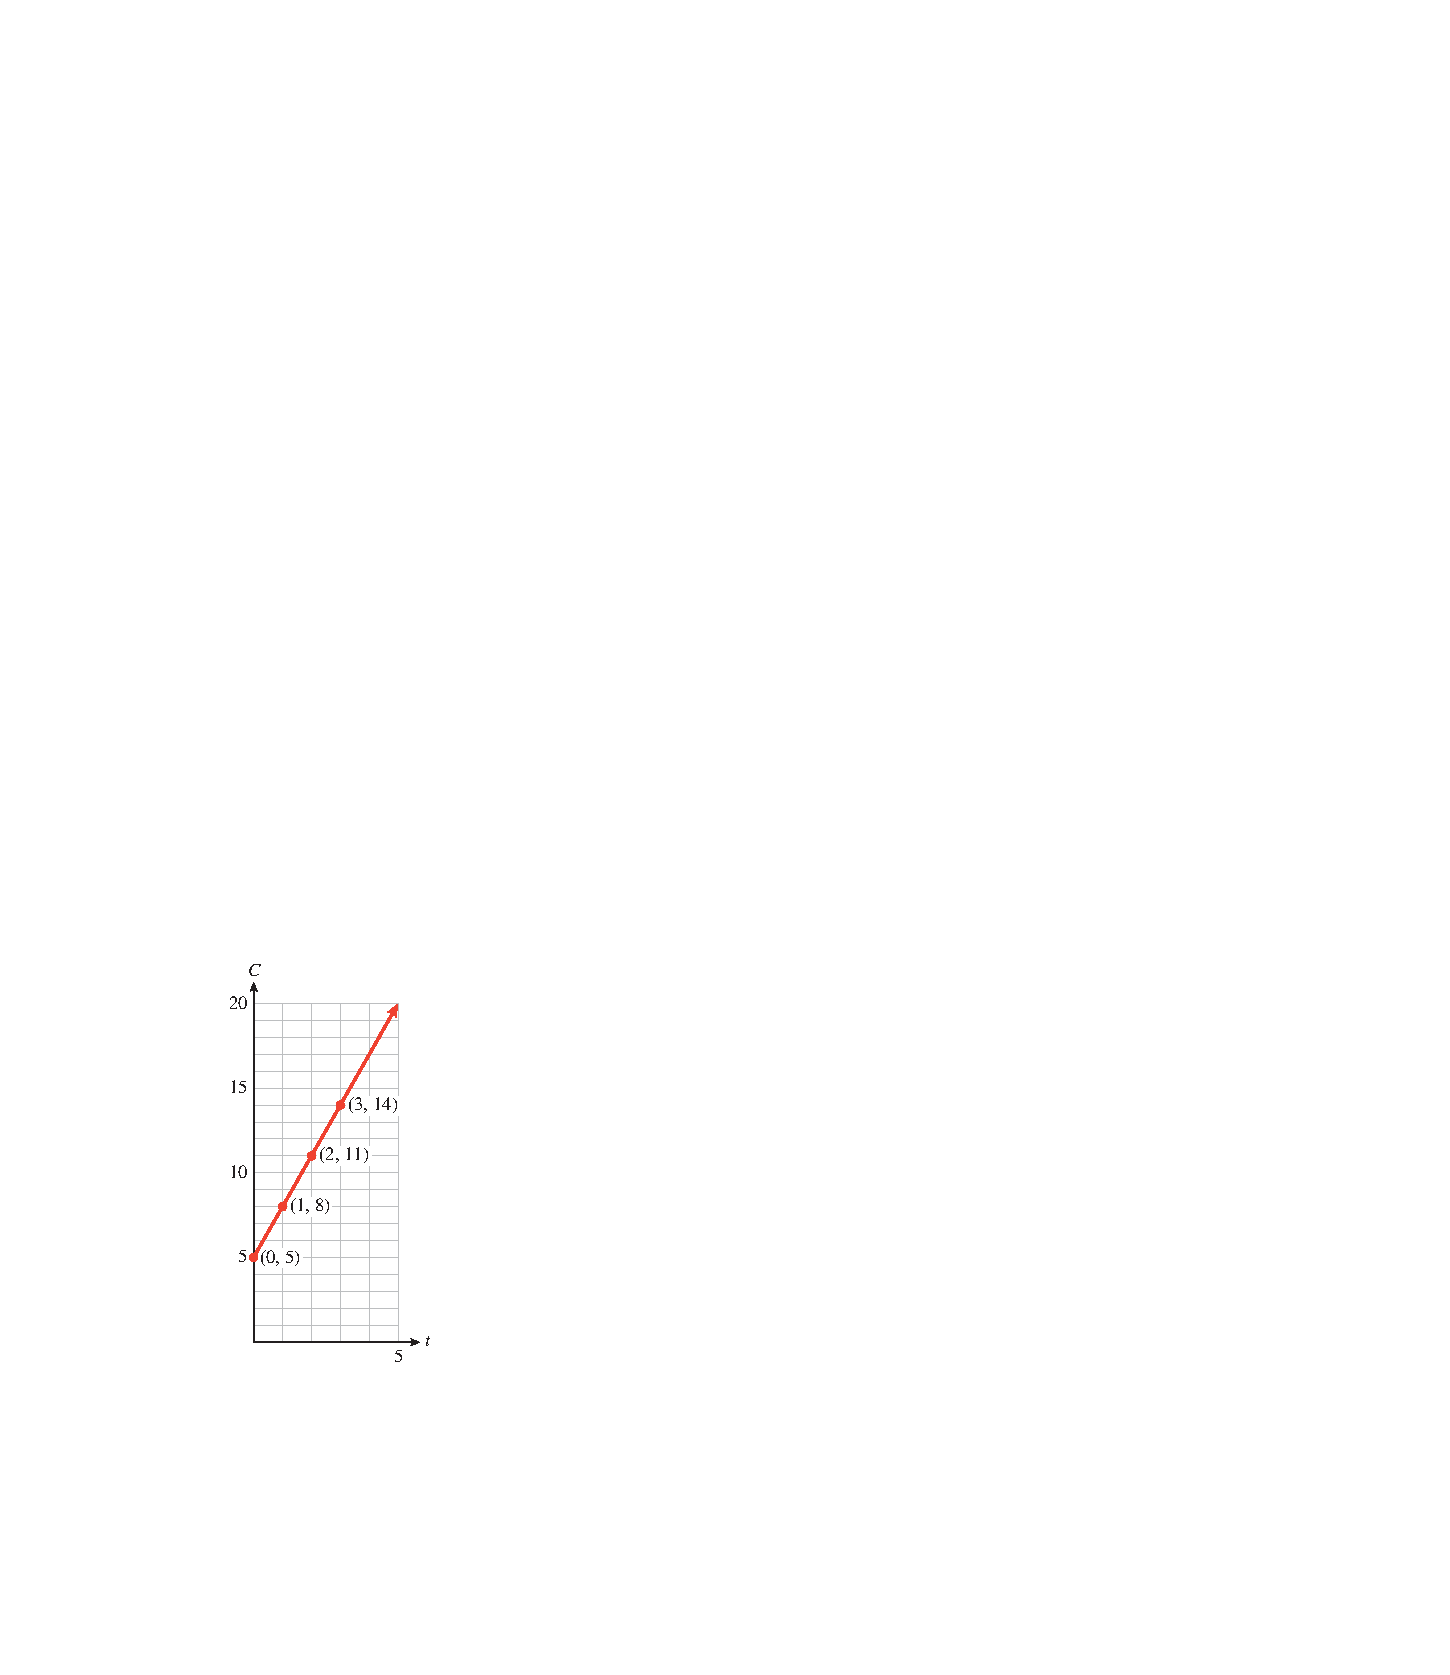
\includegraphics[width=0.4\linewidth]{images/fig-Annelise-1}
\end{figure}
\item\hypertarget{li-9}{}To write an equation, let \(C\) represent the cost of the rental, and use \(t\) for the number of hours:%
\par
%
\begin{align*}
\text{Cost}\amp=(\$5\text{ insurance fee})+(\$3\text{ per hour})\times\text{(number of hours)}\\
C\amp=5+3\cdot t=8
\end{align*}
%
\end{enumerate}
%
\end{example}
\begin{example}[]\label{example-6hrbike}
Use the equation \(C=5+3\cdot t\) you found in \hyperref[example-Annelise]{Example~\ref{example-Annelise}} to answer the following questions.  Then show how to find the answers by using the graph.%
\leavevmode%
\begin{enumerate}[label=\alph*]
\item\hypertarget{li-10}{}How much will it cost Annelise to rent a bicycle for 6 hours?%
\item\hypertarget{li-11}{}How long can Annelise bicycle for \textdollar{}18.50?%
\end{enumerate}
\par\medskip\noindent%
\textbf{Solution.}\quad \leavevmode%
\begin{enumerate}[label=\alph*]
\item\hypertarget{li-12}{}Substitute \(t=\alert{6}\) into the expression for \(C\) to find%
\begin{equation*}
C=5+3(\alert{6})=23
\end{equation*}
A 6-hour bike ride will cost \textdollar{}23.  The point \(P\) on the graph in the figure represents the cost of a 6-hour bike ride.  The value on the \(C\)-axis at the same height as point \(P\) is 23, so a 6-hour bike ride costs \textdollar{}23.%
\item\hypertarget{li-13}{}Substitute \(C=\alert{18.50}\) into the equation and solve for \(t\).%
\begin{align*}
\alert{18.50}\amp=5+3t\\
13.50\amp=3t\\
t\amp=4.5
\end{align*}
For \textdollar{}18.50 Annelise can bicycle for 4½ hours. The point \(Q\)  on the graph represents an \textdollar{}18.50 bike ride.  The value on the \(t\)-axis below point \(Q\) is 4.5, so \textdollar{}18.50 will buy a 4.5 hour bike ride.%
\end{enumerate}
 \begin{figure}
\centering
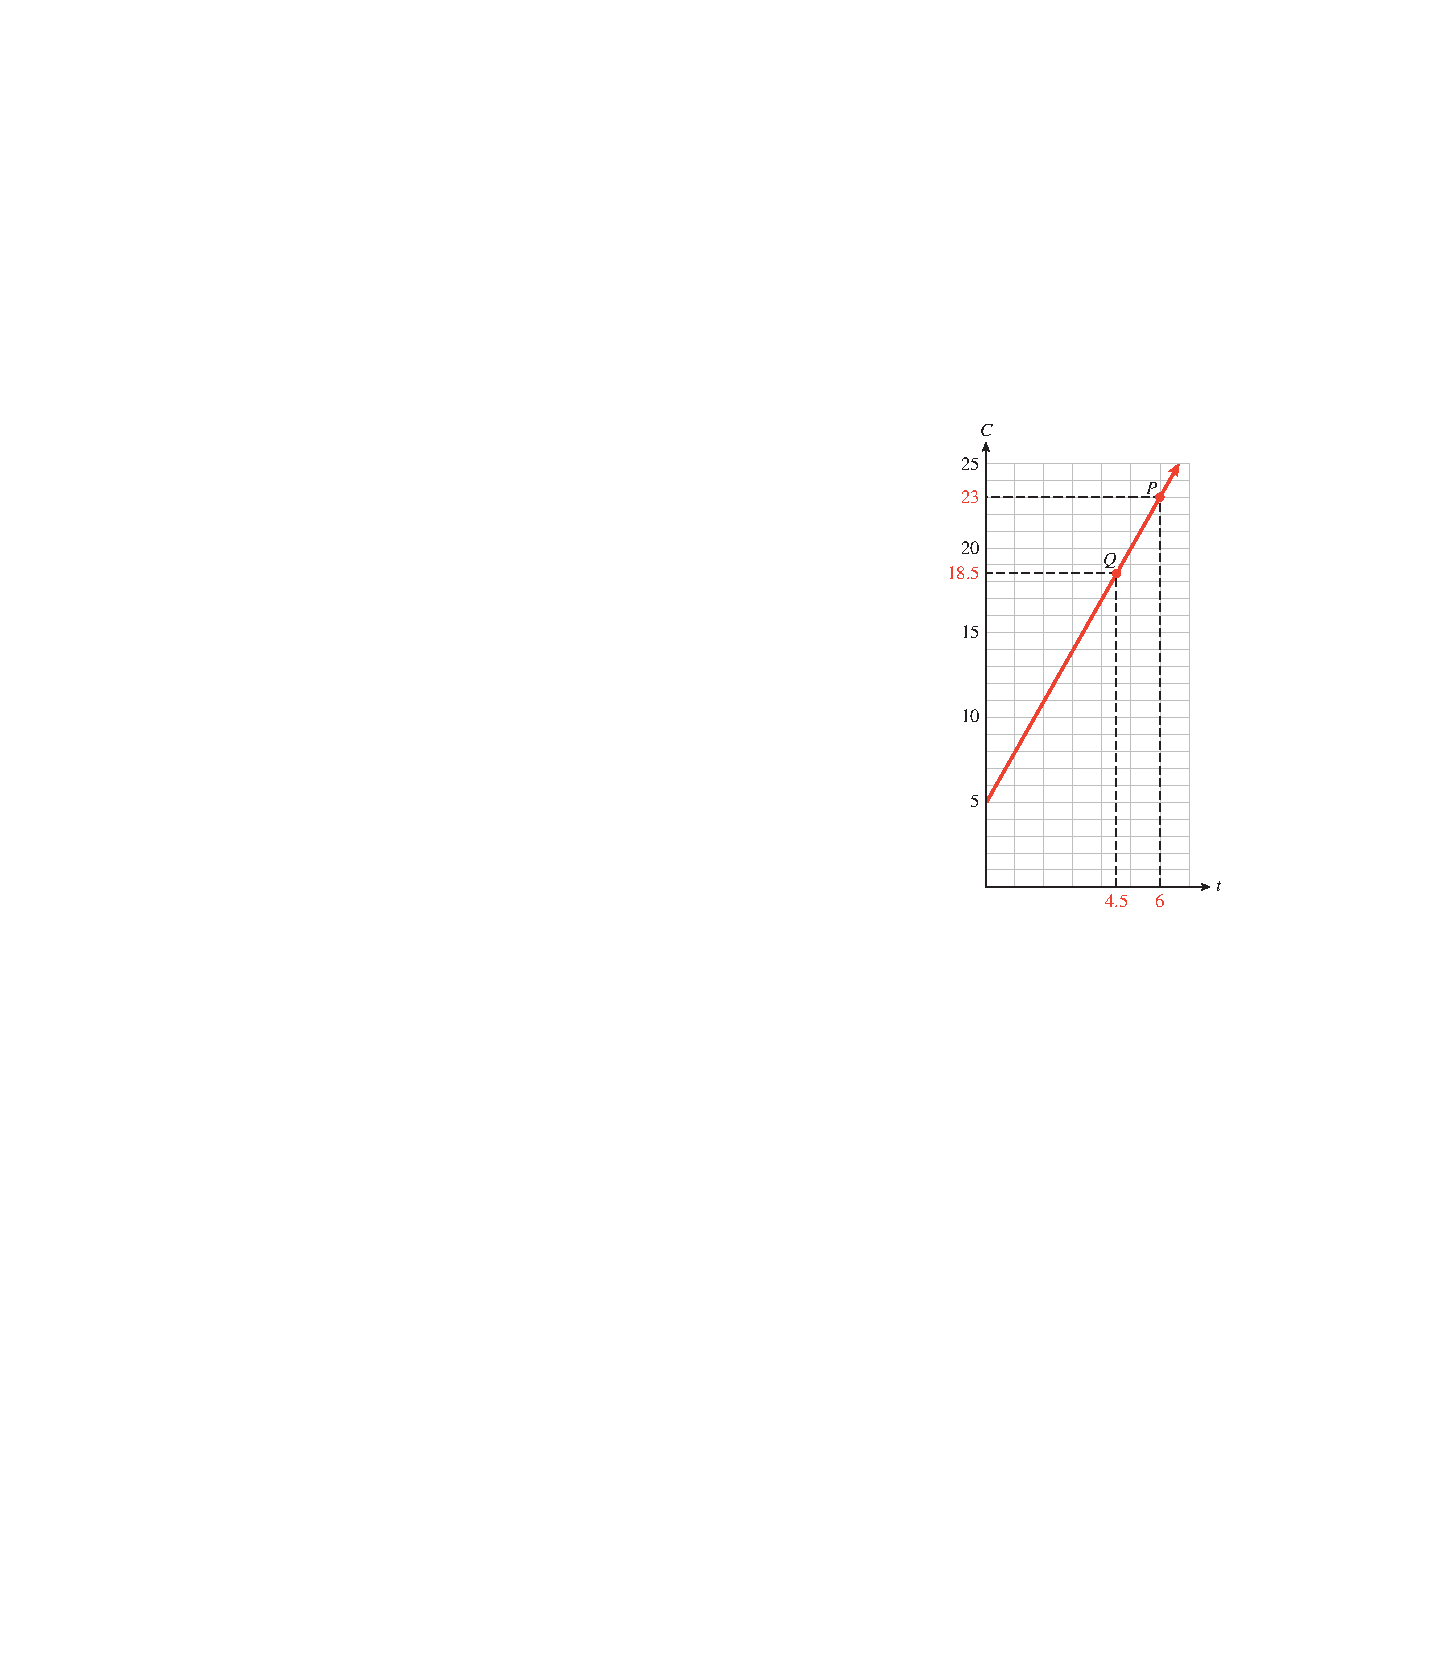
\includegraphics[width=0.4\linewidth]{images/fig1-2}
\end{figure}
%
\end{example}
In \hyperref[example-6hrbike]{Example~\ref{example-6hrbike}}, notice the different algebraic techniques we used in parts (a) and (b).   In part (a), we were given a value of \(t\) and we \terminology{evaluated the expression}  \(5+3t\) to find \(C\).  In part (b) we were given a value of \(C\) and we \terminology{solved the equation} \(C=5+3t\) to find \(t\).%
\begin{exercise}\label{exercise-Frank-plants}
Frank plants a dozen corn seedlings, each 6 inches tall.  With plenty of water and sunlight they will grow approximately 2 inches per day.  Complete the table of values for the height, \(h\), of the seedlings after \(t\) days.%
% group protects changes to lengths, releases boxes (?)
{% begin: group for a single side-by-side
% set panel max height to practical minimum, created in preamble
\setlength{\panelmax}{0pt}
\newsavebox{\panelboxBtabular}
\savebox{\panelboxBtabular}{%
\raisebox{\depth}{\parbox{0.5\textwidth}{\centering\begin{tabular}{AcAcAcAcAcAcA}\hrulethick
\(t\)&\(0\)&\(5\)&\(10\)&\(15\)&\(20\)\tabularnewline\hrulethin
\(h\)&&&&&\tabularnewline\hrulethin
\end{tabular}
}}}
\newlength{\phBtabular}\setlength{\phBtabular}{\ht\panelboxBtabular+\dp\panelboxBtabular}
\settototalheight{\phBtabular}{\usebox{\panelboxBtabular}}
\setlength{\panelmax}{\maxof{\panelmax}{\phBtabular}}
\newsavebox{\panelboxCimage}
\savebox{\panelboxCimage}{%
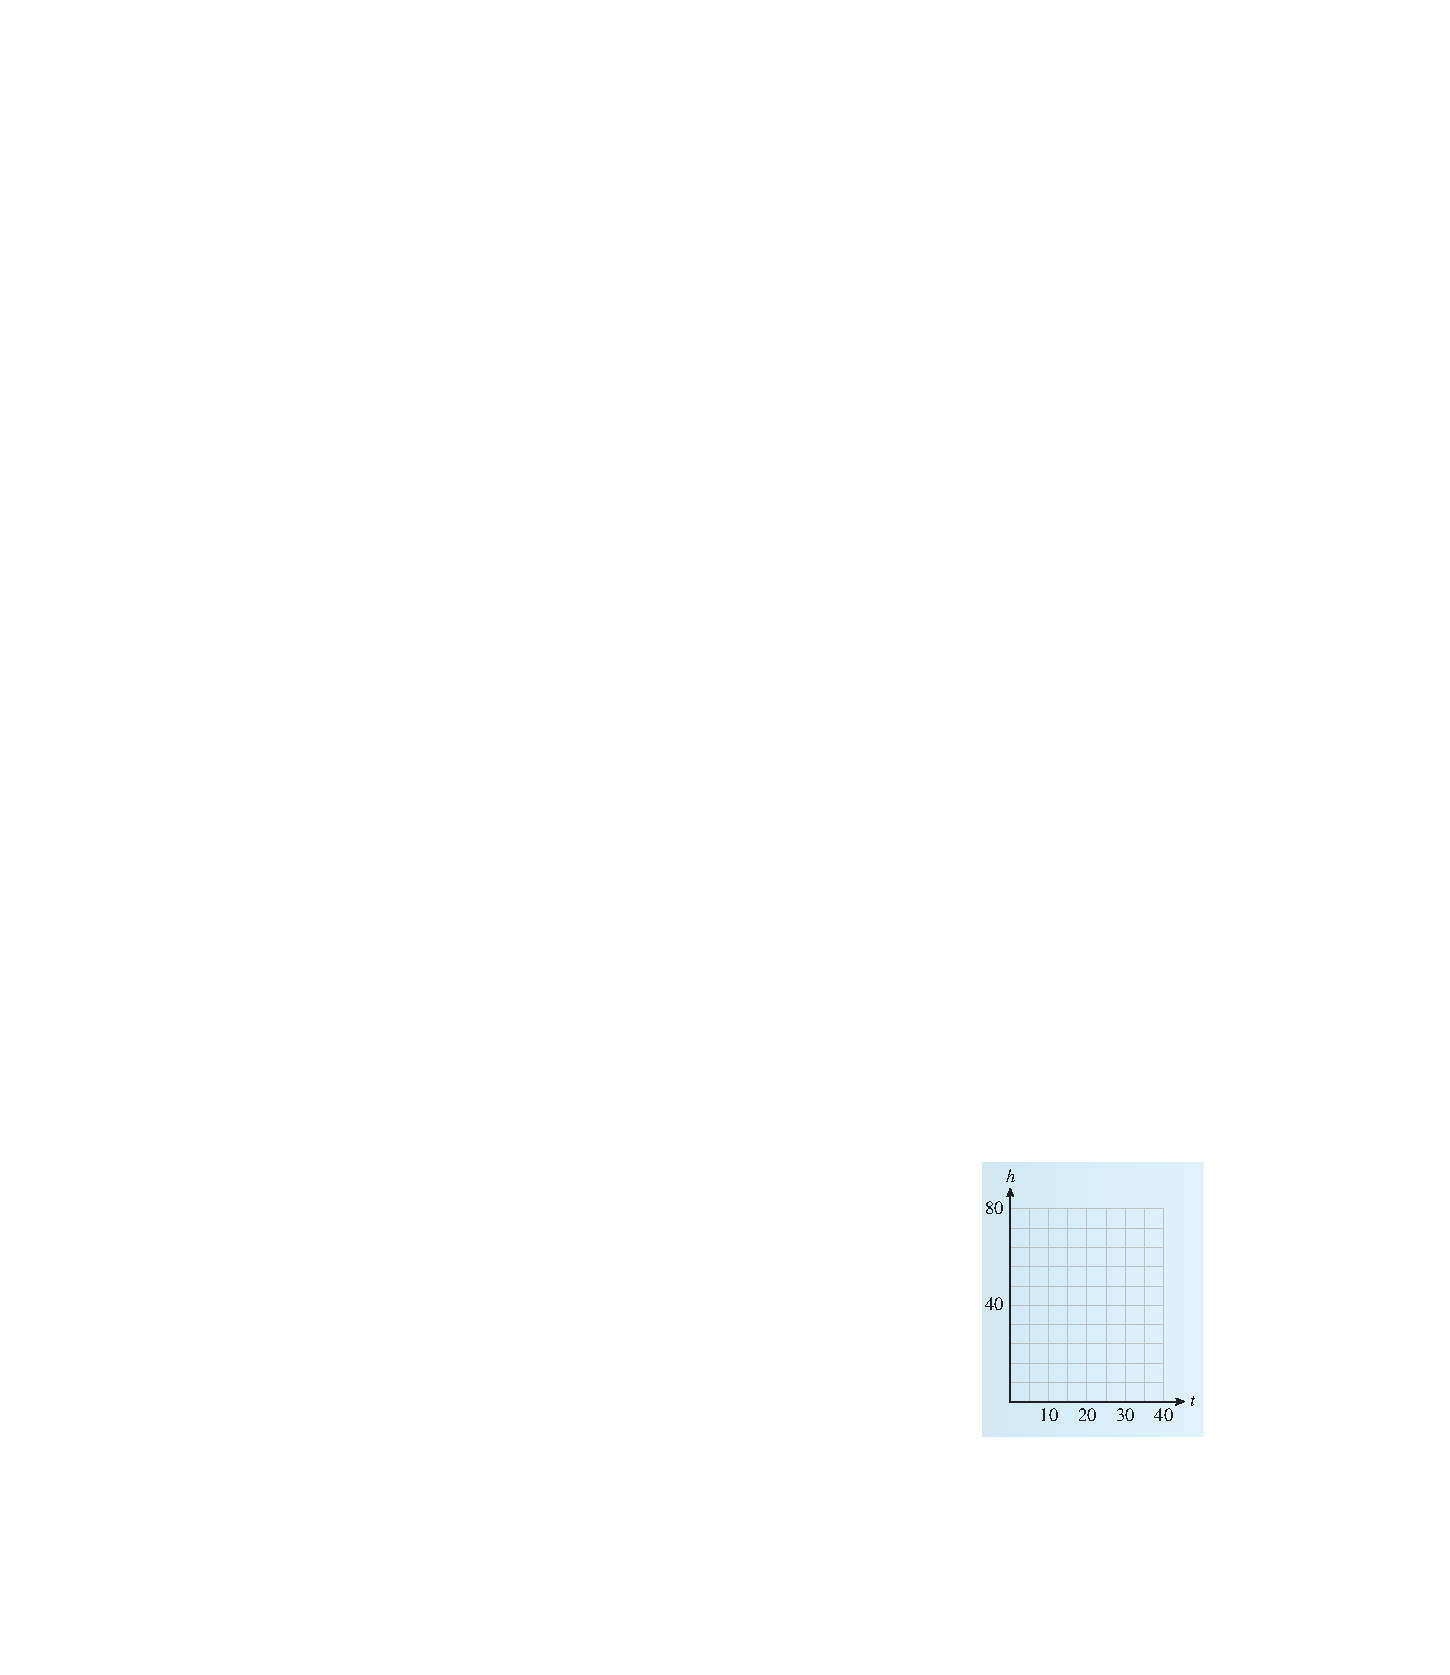
\includegraphics[width=0.5\linewidth]{images/fig-Example2}
}
\newlength{\phCimage}\setlength{\phCimage}{\ht\panelboxCimage+\dp\panelboxCimage}
\settototalheight{\phCimage}{\usebox{\panelboxCimage}}
\setlength{\panelmax}{\maxof{\panelmax}{\phCimage}}
\leavevmode%
% begin: side-by-side as figure/tabular
% \tabcolsep change local to group
\setlength{\tabcolsep}{0\textwidth}
% @{} suppress \tabcolsep at extremes, so margins behave as intended
\begin{figure}
\begin{tabular}{@{}*{2}{c}@{}}
\begin{minipage}[c][\panelmax][t]{0.5\textwidth}\usebox{\panelboxBtabular}\end{minipage}&
\begin{minipage}[c][\panelmax][t]{0.5\textwidth}\usebox{\panelboxCimage}\end{minipage}\end{tabular}
\end{figure}
% end: side-by-side as tabular/figure
}% end: group for a single side-by-side
\leavevmode%
\begin{enumerate}[label=\alph*]
\item\hypertarget{li-14}{}Write an equation for the height of the seedlings in terms of the number of days since they were planted.%
\item\hypertarget{li-15}{}Graph the equation.%
\end{enumerate}
\end{exercise}
\begin{exercise}\label{exercise-2}
Use your equation from \hyperref[exercise-Frank-plants]{Exercise~\ref{exercise-Frank-plants}} to answer the questions.  Illustrate each answer on the graph.%
\leavevmode%
\begin{enumerate}[label=\alph*]
\item\hypertarget{li-18}{}How tall is the corn after 3 weeks?%
\item\hypertarget{li-19}{}How long will it be before the corn is 6 feet tall?%
\end{enumerate}
For part (b), convert feet to inches.%
\end{exercise}
\typeout{************************************************}
\typeout{Subsection 1.1.2 Choosing Scales for the Axes}
\typeout{************************************************}
\subsection[{Choosing Scales for the Axes}]{Choosing Scales for the Axes}\label{subsection-2}
To create a useful graph, we must choose appropriate scales for the axes.  The axes must extend far enough to show the values of the variables, and the tick marks should be equally spaced.  Usually we should use no more than 10 or 15 tick marks.%
\begin{example}[]\label{example-home-price}
In 1990, the median price of a home in the US was \textdollar{}92,000.  The median price increased by about \textdollar{}4700 per year over the next decade. \leavevmode%
\begin{enumerate}[label=\alph*]
\item\hypertarget{li-22}{}Make a table of values showing the median price of a house in 1990, 1994, 1998, and 2000.%
\item\hypertarget{li-23}{}Choose suitable scales for the axes and plot the values you found in part (a) on a graph. Use \(t\), the number of years since 1990, on the horizontal axis and the price of the house, \(P\), on the vertical axis.  Draw a curve through the points.%
\item\hypertarget{li-24}{}Write an equation that expresses \(P\) in terms of \(t\).%
\item\hypertarget{li-25}{}How much did the price of the house increase from 1990 to 1996?  Illustrate the increase on your graph.%
\end{enumerate}
%
\par\medskip\noindent%
\textbf{Solution.}\quad \leavevmode%
\begin{enumerate}[label=\alph*]
\item\hypertarget{li-26}{}In 1990 the median price was \textdollar{}92,000.  Four years later, in 1994, the price had increased by \(\alert{4}(4700)=18,800\) dollars, so%
\begin{equation*}
P=92,000+\alert{4}(4700)=110,800
\end{equation*}
In 1998 the price had increased by \(\alert{8}(4700)=37,600\)  dollars, so%
\begin{equation*}
P=92,000+\alert{8}(4700)=129,600
\end{equation*}
You can verify the price of the house in 2000 by a similar calculation.%
\begin{table}
\centering
\begin{tabular}{AcAcAcA}\hrulethick
Year&Price of House)&\((t,P)\)\tabularnewline\hrulethin
\(1990\)&\(92,000\)&\((0,\, 92,000)\)\tabularnewline\hrulethin
\(1994\)&\(110,800\)&\((4,\, 110,800)\)\tabularnewline\hrulethin
\(1998\)&\(129,600\)&\((8,\, 129,600)\)\tabularnewline\hrulethin
\(2000\)&\(139,000\)&\((10,\, 139,000)\)\tabularnewline\hrulethin
\end{tabular}
\end{table}
\item\hypertarget{li-27}{}Let \(t\) stand for the number of years since 1990, so that \(t=0\) in 1990, \(t=4\) in 1994, and so on.  To choose scales for the axes, look at the values in the table.  For this graph we scale the horizontal axis, or \(t\)-axis, in 1-year intervals and the vertical axis, or \(P\)-axis, for \textdollar{}90,000 to \textdollar{}140,000 in intervals of \textdollar{}5,000. The points in \hyperref[fig-median-house]{Figure~\ref{fig-median-house}}. lie on a straight line.%
\item\hypertarget{li-28}{}Look back at the calculations in part (a).  The price of the house started at \textdollar{}92,000 in 1990 and increased by \(t \times 4700\) dollars after \(t\) years.  Thus,%
\begin{equation*}
P=92,000+4700t
\end{equation*}
%
\item\hypertarget{li-29}{}Find the points on the graph corresponding to 1990 and 1996.%
\begin{figure}
\centering
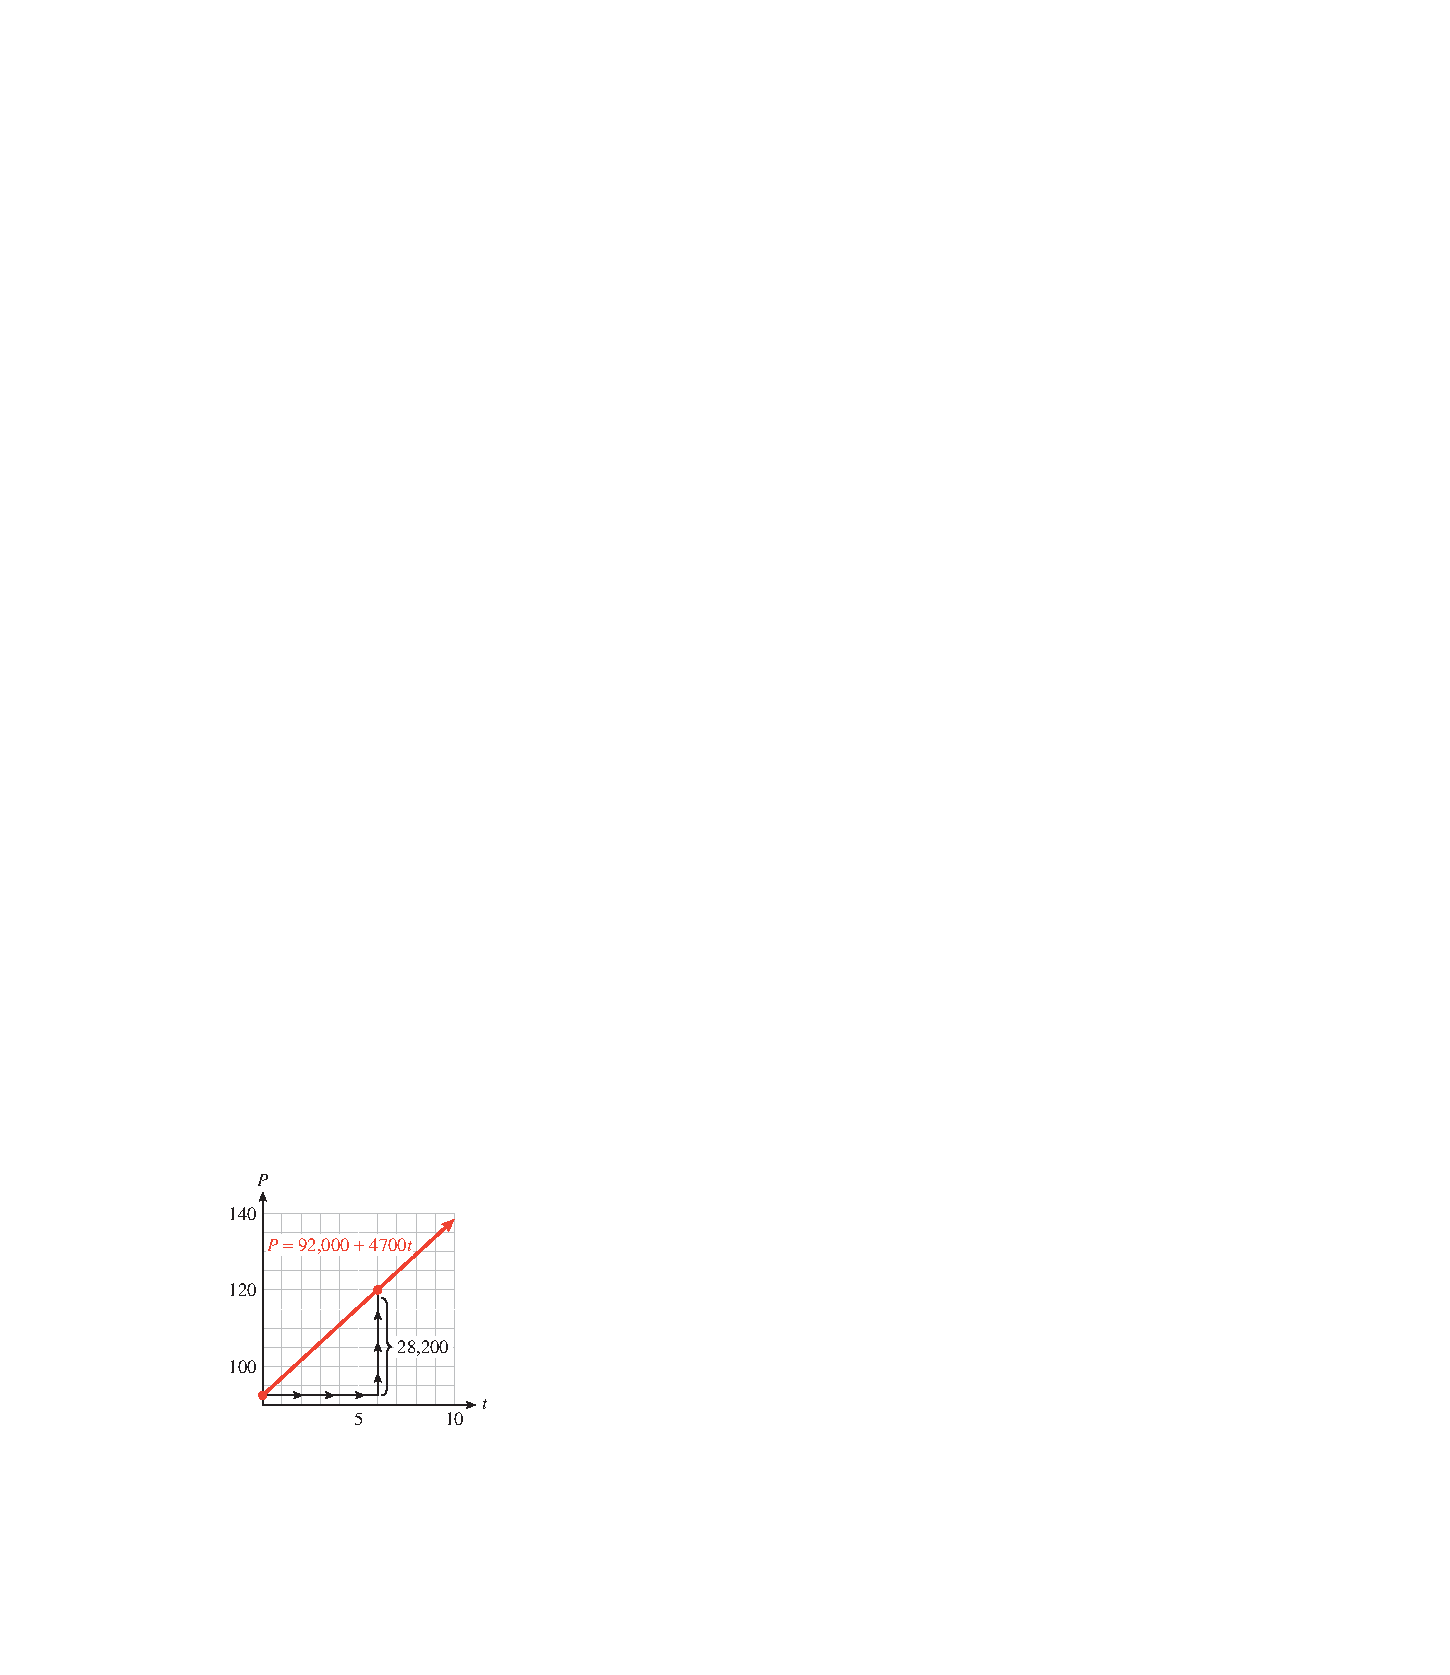
\includegraphics[width=0.5\linewidth]{images/fig1-3}
\caption{\label{fig-median-house}}
\end{figure}
These points lie above \(t=0\) and \(t=6\) on the \(t\)-axis.  Now find the values on the \(P\)-axis corresponding to the two points.  The values are \(P=92,000\) in 1990 and \(P=120,200\) in 1996.  The increase in price is the difference of the two \(P\)-values.%
\begin{align*}
\text{increase in price}\amp=120,200-92,000
\\
\amp=28,200
\end{align*}
The price of the home increased \textdollar{}28,200 between 1990 and 1996.  This increase is indicated by the arrows in \hyperref[fig-median-house]{Figure~\ref{fig-median-house}}.%
\end{enumerate}
\end{example}
The graphs in the preceding examples are \terminology{increasing graphs}.  As we move along the graph from left to right (in the direction of increasing \(t\) ), the second coordinate increases as well.  Try \hyperref[exercise-Silver-Lake]{Exercise~\ref{exercise-Silver-Lake}}, which illustrates a \terminology{decreasing graph}.%
\begin{exercise}\label{exercise-Silver-Lake}
Silver Lake has been polluted by industrial waste products.  The concentration of toxic chemicals in the water is currently 285 parts per million (ppm).  Local environmental officials would like to reduce the concentration by 15 ppm each year%
\leavevmode%
\begin{enumerate}[label=\alph*]
\item\hypertarget{li-30}{}Complete the table of values showing the desired concentration, \(C,\)~ of toxic chemicals \(t\) years from now.  For each \(t\)-value, calculate the corresponding value for \(C\).  Write your answers as ordered pairs.%
\begin{table}
\centering
\begin{tabular}{AcAcAcAcA}\hrulethick
\(t\)&\(C\)&&\((t,C)\)\tabularnewline\hrulethin
\(0\)&&\(C=285-150(\alert{0})\)&\((0, ~~~~ )\)\tabularnewline\hrulethin
\(5\)&&\(C=285-150(\alert{5})\)&\((5, ~~~~ )\)\tabularnewline\hrulethin
\(10\)&&\(C=285-150(\alert{10})\)&\((10, ~~~~ )\)\tabularnewline\hrulethin
\(15\)&&\(C=285-150(\alert{15})\)&\((15, ~~~~ )\)\tabularnewline\hrulethin
\end{tabular}
\end{table}
\item\hypertarget{li-31}{}To choose scales for the axes, notice that the value of \(C\) starts at 285 and decreases from there.  We'll scale the vertical axis up to 300, and use 10 tick marks at intervals of 30.  Graph the ordered pairs on the grid, and connect them with a straight line. Extend the graph until it reaches the horizontal axis, but no farther.  Points with negative \(C\)-coordinates have no meaning for the problem.%
\item\hypertarget{li-32}{}Write an equation for the concentration, \(C\), of toxic chemicals \(t\) years from now.%
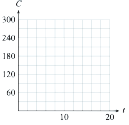
\includegraphics[width=0.5\linewidth]{images/fig-Exercise3}
\end{enumerate}
\par\smallskip
\noindent\textbf{Hint.}\hypertarget{hint-2}{}\quad
For part (c): The concentration is initially 8 ppm, and we subtract 15 ppm for each year that passes, or \(15 \times t\).%
\end{exercise}
\begin{remark}[Graphing an Equation]\label{remark-1}
We can use a graphing calculator to graph an equation. On most calculators, we follow three steps.%
\par
To Graph an Equation:%
\leavevmode%
\begin{enumerate}
\item\hypertarget{li-36}{}Press \lstinline?Y=? and enter the equation you wish to graph.%
\item\hypertarget{li-37}{}Press \lstinline?WINDOW? and select a suitable graphing window.%
\item\hypertarget{li-38}{}Press \lstinline?GRAPH?%
\end{enumerate}
\end{remark}
\begin{example}[Using a Graphing Calculator]\label{graphing-calculator}
In \hyperref[example-home-price]{Example~\ref{example-home-price}}, we found the equation \(P = 92,000 + 4700t\) for the median price of a house \(t\) years after 1990. Graph this equation on a calculator.%
\par\medskip\noindent%
\textbf{Solution.}\quad To begin, we press \lstinline?Y=? and enter%
\begin{equation*}
Y1 = 92,000 + 4700X
\end{equation*}
%
\par
For this graph, we’ll use the grid in \hyperref[example-home-price]{Example~\ref{example-home-price}} for our window settings, so we press \lstinline?WINDOW? and enter%
\begin{table}
\centering
\begin{tabular}{lll}
Xmin\(=0\)&&Xmax\(=10\)\tabularnewline[0pt]
Ymin\(=90,000\)&&Ymax\(=140,000\)
\end{tabular}
\end{table}
Finally, we press \lstinline?GRAPH?. The calculator's graph is shown in \hyperref[fig-GC-house-price]{Figure~\ref{fig-GC-house-price}}. \begin{figure}
\centering
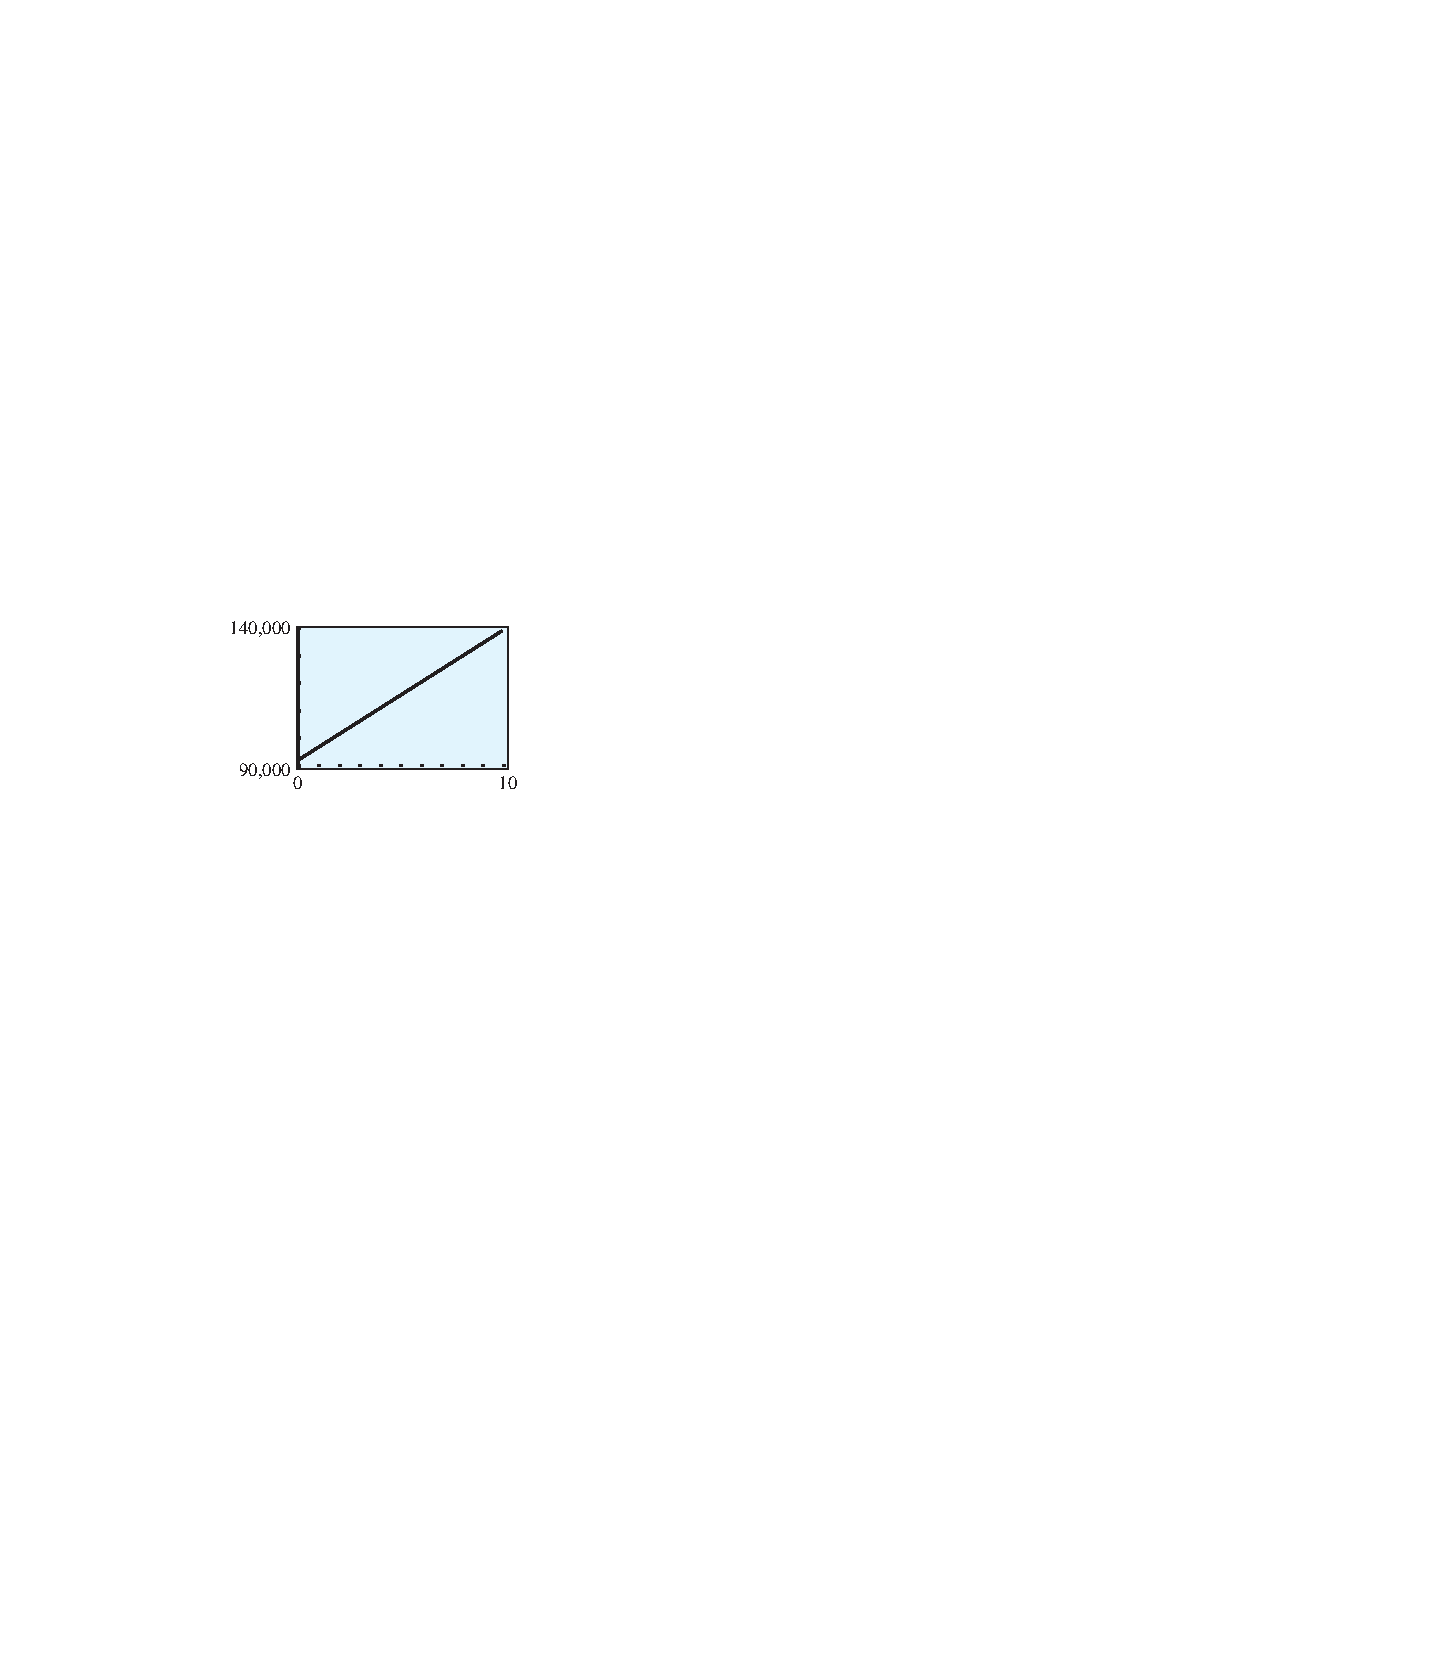
\includegraphics[width=0.5\linewidth]{images/fig-GC-house-price}
\caption{\label{fig-GC-house-price}}
\end{figure}
%
\end{example}
\begin{exercise}\label{exercise-gc}
\leavevmode%
\begin{enumerate}[label=\alph*]
\item\hypertarget{li-39}{}Solve the equation \(2y - 1575 = 45x\) for \(y\) in terms of \(x\).%
\item\hypertarget{li-40}{}Graph the equation on a graphing calculator. Use the window \leavevmode%
\begin{table}
\centering
\begin{tabular}{lllll}
Xmin\(=-50\)&&Xmax\(=50\)&&Xscl\(=5\)\tabularnewline[0pt]
Ymin\(=-500\)&&Ymax\(=1000\)&&Yscl\(=100\)
\end{tabular}
\end{table}
%
\item\hypertarget{li-41}{}Sketch the graph on paper. Use the window settings to choose appropriate scales for the axes.%
\end{enumerate}
\end{exercise}
\typeout{************************************************}
\typeout{Subsection 1.1.3 Linear Equations}
\typeout{************************************************}
\subsection[{Linear Equations}]{Linear Equations}\label{subsection-3}
All the models in the preceding examples have equations with a similar form:%
\begin{equation*}
y=\text{(starting value)}+\text{(rate of change)}\cdot x
\end{equation*}
(We'll talk more about rate of change in {$\langle\langle$Unresolved xref, reference "slope-and-rate-of-change"; check spelling or use "provisional" attribute$\rangle\rangle$}.)  Their graphs were all portions of straight lines.  For this reason such equations are called  \terminology{linear equations}.  The order of the terms in the equation does not matter.  For example, the equation in \hyperref[example-Annelise]{Example~\ref{example-Annelise}},%
\begin{equation*}
C=5+3t
\end{equation*}
can be written equivalently as%
\begin{equation*}
-3t+C=5
\end{equation*}
and the equation in \hyperref[example-home-price]{Example~\ref{example-home-price}},%
\begin{equation*}
P=92,000+4700t
\end{equation*}
can be written as%
\begin{equation*}
-4700t +P=92,000
\end{equation*}
This form of a linear equation,%
\begin{equation*}
Ax+By=C
\end{equation*}
is called the \terminology{general form}.%
\begin{assemblage}{General Form for a Linear Equation}\label{assemblage-1}
The graph of any equation%
\begin{equation*}
Ax+By=C
\end{equation*}
where \(A\) and \(B\) are not both equal to zero, is a straight line.%
\end{assemblage}
\begin{example}[]\label{example-advertising}
The manager at Albert's Appliances has \textdollar{}3000 to spend on advertising for the next fiscal quarter.  A 30-second spot on television costs \textdollar{}150 per broadcast, and a 30-second radio ad costs \textdollar{}50.%
\leavevmode%
\begin{enumerate}[label=\alph*]
\item\hypertarget{li-45}{}The manager decides to buy \(x\) television ads and \(y\) radio ads.  Write an equation relating \(x\) and \(y\).%
\item\hypertarget{li-46}{}Make a table of values showing several choices for \(x\) and \(y\).%
\item\hypertarget{li-47}{}Plot the points from your table, and graph the equation.%
\end{enumerate}
\par\medskip\noindent%
\textbf{Solution.}\quad \leavevmode%
\begin{enumerate}[label=\alph*]
\item\hypertarget{li-48}{}Each television ad costs \textdollar{}150, so \(x\) ads will cost \(\$150x\).  Similarly, \(y\) radio ads will cost \(\$50y\).  The manager has \textdollar{}3000 to spend, so the sum of the costs must be \textdollar{}3000.  Thus,%
\begin{equation*}
150x+50y=3000
\end{equation*}
%
\item\hypertarget{li-49}{}Choose some values of \(x\), and solve the equation for the corresponding value of \(y\).  For example, if \(x=\alert{10}\) then%
\begin{align*}
150(\alert{10})+50y\amp=300\\
1500+50y\amp=3000\\
50y\amp=1500\\
y\amp=30
\end{align*}
If the manager buys 10 television ads, she can also buy 30 radio ads.  You can verify the other entries in the table.%
\begin{table}
\centering
\begin{tabular}{AcAcAcAcAcA}\hrulethick
\(x\)&\(8\)&\(10\)&\(12\)&\(14\)\tabularnewline\hrulethin
\(y\)&\(36\)&\(30\)&\(24\)&\(18\)\tabularnewline\hrulethin
\end{tabular}
\end{table}
\item\hypertarget{li-50}{}Plot the points from the table.  All the solutions lie on a straight line, as shown in \hyperref[fig-example-advertising]{Figure~\ref{fig-example-advertising}} . \begin{figure}
\centering
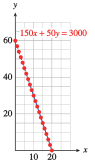
\includegraphics[width=0.4\linewidth]{images/fig-example-advertising}
\caption{\label{fig-example-advertising}}
\end{figure}
%
\end{enumerate}
%
\end{example}
\begin{exercise}\label{exercise-crops}
In central Nebraska, each acre of corn requires 25 acre-inches of water per year, and each acre of winter wheat requires 18 acre-inches of water.             (An acre-inch is the amount of water needed to cover one acre of land to a depth of one inch.)  A farmer can count on 9000 acre-inches of water for the coming year.  (Source:  Institute of Agriculture and Natural Resources, University of Nebraska) \leavevmode%
\begin{enumerate}[label=\alph*]
\item\hypertarget{li-51}{}Write an equation relating the number of acres of corn, \(x\), and the number of acres of wheat, \(y\), that the farmer can plant.%
\item\hypertarget{li-52}{}Complete the table.%
\begin{table}
\centering
\begin{tabular}{AcAcAcAcAcA}\hrulethick
\(x\)&\(50\)&\(100\)&\(150\)&\(200\)\tabularnewline\hrulethin
\(y\)&\(\hphantom{0000}\)&\(\hphantom{0000}\)&\(\hphantom{0000}\)&\(\hphantom{0000}\)\tabularnewline\hrulethin
\end{tabular}
\end{table}
\end{enumerate}
%
\end{exercise}
\typeout{************************************************}
\typeout{Subsection 1.1.4 Intercepts}
\typeout{************************************************}
\subsection[{Intercepts}]{Intercepts}\label{subsection-4}
% group protects changes to lengths, releases boxes (?)
{% begin: group for a single side-by-side
% set panel max height to practical minimum, created in preamble
\setlength{\panelmax}{0pt}
\newsavebox{\panelboxLimage}
\savebox{\panelboxLimage}{%
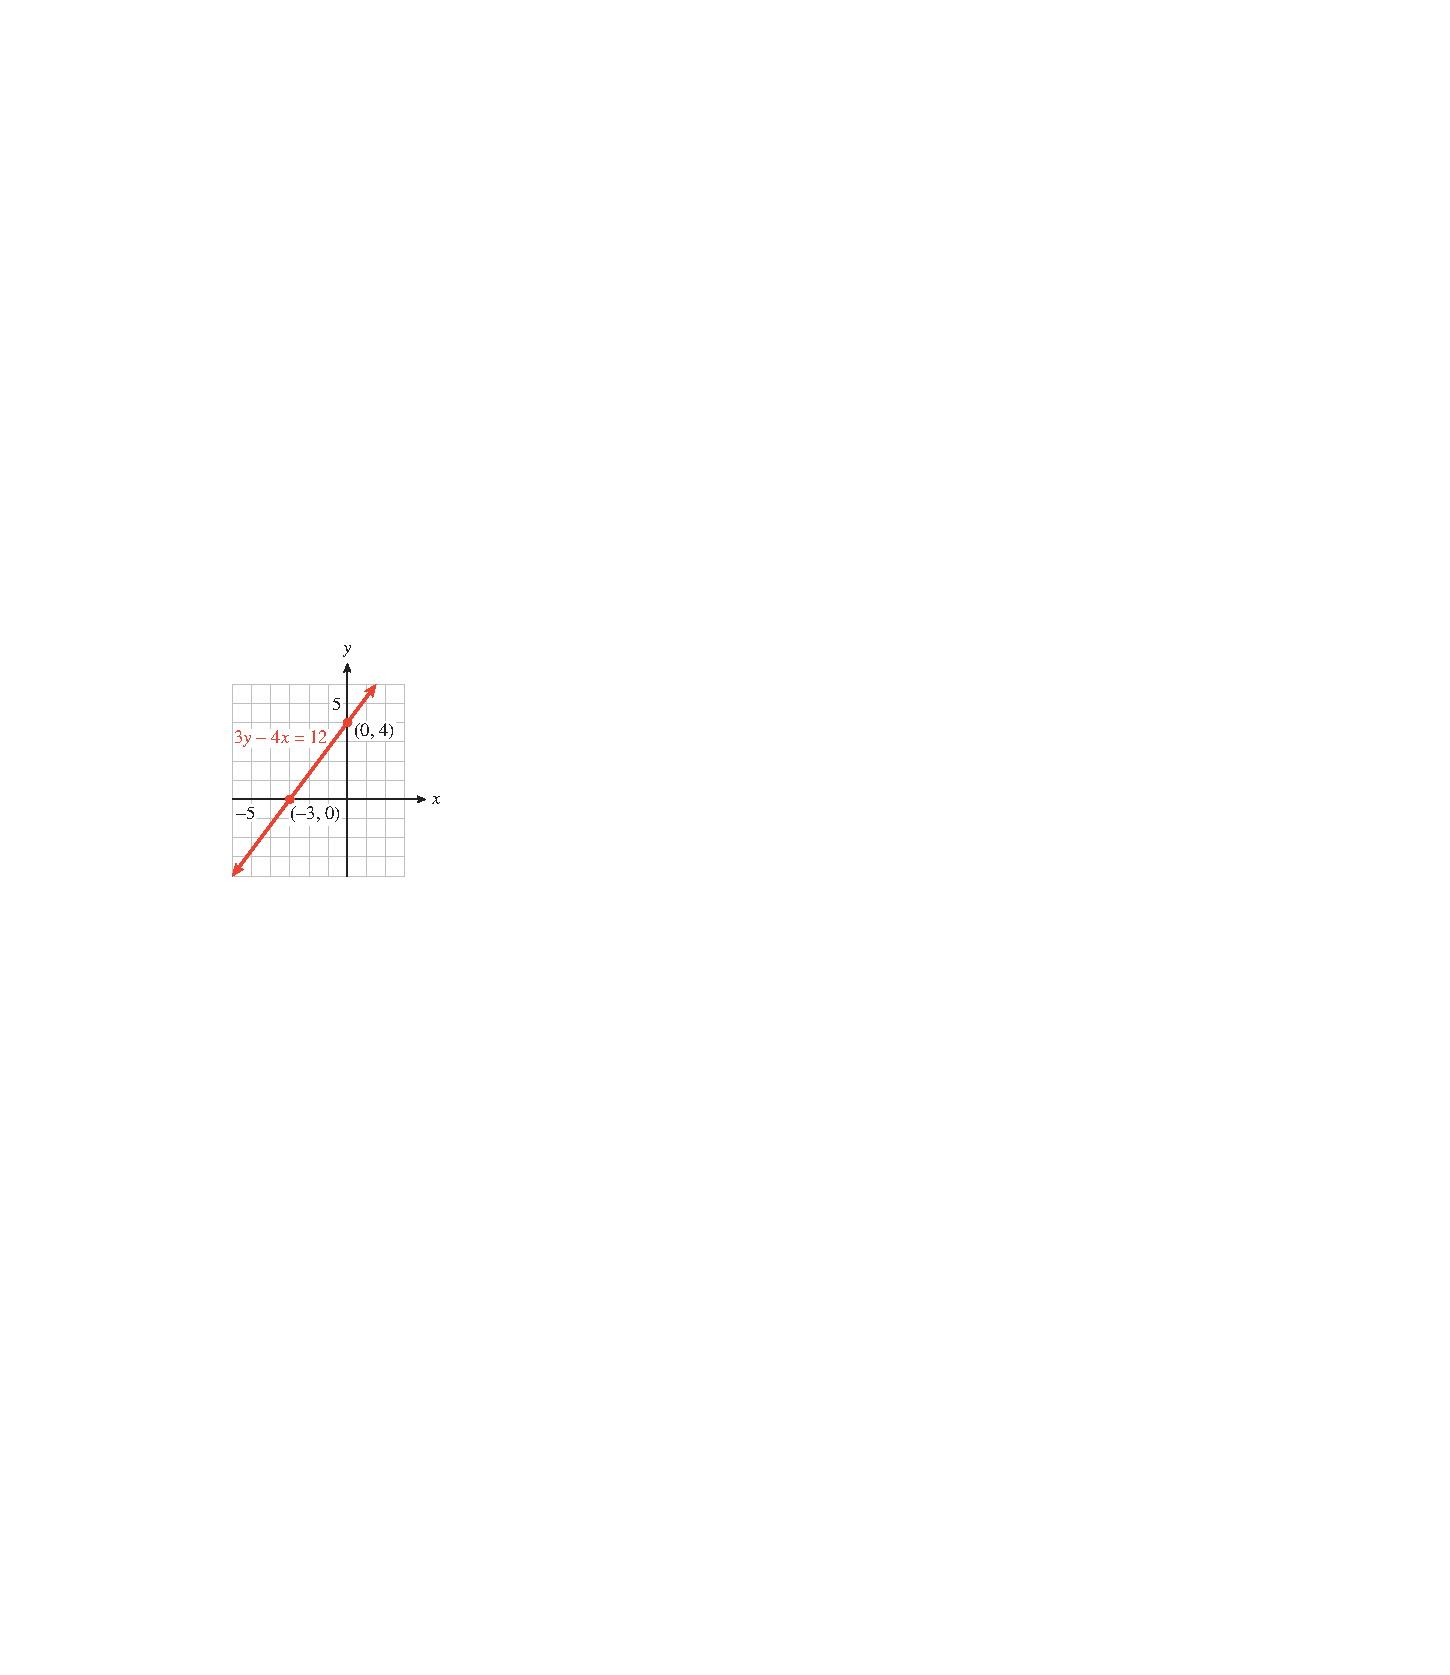
\includegraphics[width=0.35\linewidth]{images/fig-intercepts}
}
\newlength{\phLimage}\setlength{\phLimage}{\ht\panelboxLimage+\dp\panelboxLimage}
\settototalheight{\phLimage}{\usebox{\panelboxLimage}}
\setlength{\panelmax}{\maxof{\panelmax}{\phLimage}}
\newsavebox{\panelboxCJp}
\savebox{\panelboxCJp}{%
\raisebox{\depth}{\parbox{0.6\textwidth}{Consider the graph of the equation%
\begin{equation*}
3x-4y=12
\end{equation*}
shown in \hyperref[fig-intercepts]{Figure~\ref{fig-intercepts}}. The points where the graph crosses the axes are called the \terminology{intercepts} of the graph. The coordinates of these points are easy to find.  The \(y\)-coordinate of the \(x\)-intercept is zero, so we set \(y=\alert{0}\) in the equation to get%
\begin{align*}
3(\alert{0})-4x\amp=12\\
x=-3
\end{align*}
}}}
\newlength{\phCJp}\setlength{\phCJp}{\ht\panelboxCJp+\dp\panelboxCJp}
\settototalheight{\phCJp}{\usebox{\panelboxCJp}}
\setlength{\panelmax}{\maxof{\panelmax}{\phCJp}}
\leavevmode%
% begin: side-by-side as figure/tabular
% \tabcolsep change local to group
\setlength{\tabcolsep}{0.025\textwidth}
% @{} suppress \tabcolsep at extremes, so margins behave as intended
\begin{figure}
\begin{tabular}{@{}*{2}{c}@{}}
\begin{minipage}[c][\panelmax][t]{0.35\textwidth}\usebox{\panelboxLimage}\end{minipage}&
\begin{minipage}[c][\panelmax][t]{0.6\textwidth}\usebox{\panelboxCJp}\end{minipage}\tabularnewline
\parbox[t]{0.35\textwidth}{\captionof{figure}{\label{fig-intercepts}}
}&
\end{tabular}
\end{figure}
% end: side-by-side as tabular/figure
}% end: group for a single side-by-side
The \(x\)-intercept is the point \((-3,0)\). Also, the \(x\)-coordinate of the \(y\)-intercept is zero, so we set \(x=\alert{0}\) in the equation to get%
\begin{gather*}
3y-4(\alert{0})=12\\
y=4
\end{gather*}
The \(y\)-intercept is \((0,4)\).%
\begin{assemblage}{Intercepts of a Graph}\label{assemblage-2}
The points where a graph crosses the axes are called the \terminology{intercepts of the graph}. \leavevmode%
\begin{enumerate}
\item\hypertarget{li-55}{}To find the \(y\)-intercept, set \(x=0\) and solve for \(y\).%
\item\hypertarget{li-56}{}To find the \(x\)-intercept, set \(y=0\) and solve for \(x\)%
\end{enumerate}
%
\end{assemblage}
The intercepts of a graph tell us something about the situation it models.%
\begin{example}[]\label{example-intercepts}
\leavevmode%
\begin{enumerate}[label=\alph*]
\item\hypertarget{li-57}{}Find the intercepts of the graph in \hyperref[exercise-Silver-Lake]{Exercise~\ref{exercise-Silver-Lake}}, about the pollution in Silver Lake.%
\item\hypertarget{li-58}{}What do the intercepts tell us about the problem?%
\end{enumerate}
\par\medskip\noindent%
\textbf{Solution.}\quad \leavevmode%
\begin{enumerate}[label=\alph*]
\item\hypertarget{li-59}{}An equation for the concentration of toxic chemicals is%
\begin{equation*}
C=285-15t
\end{equation*}
To find the \(C\)-intercept, set \(t\) equal to zero.%
\begin{equation*}
C=285-15(0)=285
\end{equation*}
The \(C\)-intercept is the point \((0, 285)\), or simply 285.  To find the \(t\)-intercept, set \(C\) equal to zero and solve for \(t\). \begin{align*} \alert{0}\&=285-15t \&\&\text{Add }15t \text{ to both sides.}\textbackslash{}\textbackslash{} 15t\&=285  \&\&\text{Divide both sides by 15.}\textbackslash{}\textbackslash{} t\&=19   \&\& \end{align*}%
 \par
The \(t\)-intercept is the point \((19,0)\), or simply \(19\).%
%
\item\hypertarget{li-60}{}The \(C\)-intercept represents the concentration of toxic chemicals in Silver Lake now:  When  \(t=0\), \(C=285\),  so the concentration is currently \(285\) ppm.  The \(t\)-intercept represents the number of years it will take for the concentration of toxic chemicals to drop to zero:  When \(C=0\), \(t=19\),  so it will take \(19\) years for the pollution to be eliminated entirely.%
\end{enumerate}
\end{example}
\begin{exercise}\label{exercise-6}
\leavevmode%
\begin{enumerate}[label=\alph*]
\item\hypertarget{li-61}{}Find the intercepts of the graph in \hyperref[example-advertising]{Example~\ref{example-advertising}}, about the advertising budget for Albert's Appliances: \(150x + 50y = 3000\).%
\item\hypertarget{li-62}{}What do the intercepts tell us about the problem?%
\end{enumerate}
\end{exercise}
\typeout{************************************************}
\typeout{Subsection 1.1.5 Intercept Method for Graphing Lines}
\typeout{************************************************}
\subsection[{Intercept Method for Graphing Lines}]{Intercept Method for Graphing Lines}\label{subsection-5}
Because we really only need two points to graph a linear equation, we might as well find the intercepts first and use them to draw the graph. The values of the intercepts will also help us choose suitable scales for the axes. It is always a good idea to find a third point as a check.%
\begin{example}[]\label{intercepts}
\leavevmode%
\begin{enumerate}[label=\alph*]
\item\hypertarget{li-63}{}Find the \(x\)- and \(y\)-intercepts of the graph of \(150x - 180y = 9000\).%
\item\hypertarget{li-64}{}Use the intercepts to graph the equation. Find a third point as a check.%
\end{enumerate}
\par\medskip\noindent%
\textbf{Solution.}\quad \leavevmode%
\begin{enumerate}[label=\alph*]
\item\hypertarget{li-65}{}To find the \(x\)-intercept, set \(y = \alert{0}\).%
\par
\begin{align*} 150x-18(\alert{0})\&=9000 \&\&\text{Simpify.}\textbackslash{}\textbackslash{} 150x\&=9000  \&\&\text{Divide both sides by 150.}\textbackslash{}\textbackslash{} x\&=60   \&\& \end{align*}%
\par
The \(x\)-intercept is the point \((60, 0)\). To find the \(y\)-intercept, set \(x = \alert{0}\).%
\par
\begin{align*} 150(\alert{0})-18y\&=9000 \&\&\text{Simpify.}\textbackslash{}\textbackslash{} -180y\&=9000  \&\&\text{Divide both sides by } -180\text{.}\textbackslash{}\textbackslash{} y\&=-50   \&\& \end{align*}%
\par
The \(y\)-intercept is the point \((0, -50)\).%
\item\hypertarget{li-66}{}Scale both axes in intervals of 10 and then plot the two intercepts, \((60, 0)\) and \((0, -50)\). Draw the line through them, as shown in \hyperref[fig-example-graph-intercepts]{Figure~\ref{fig-example-graph-intercepts}}. Now find another point and check that it lies on this line. We choose \(x = \alert{20}\) and solve for \(y\).%
\begin{align*}
150(\alert{20}) -180y \amp = 9000\\
3000 -180y \amp = 9000\\
-180y \amp = 6000\\
y \amp =-33.\overline{3}
\end{align*}
Plot the point \((20, -33\frac{1}{3})\). Because this point lies on the line, we can be reasonably confident that our graph is correct. \begin{figure}
\centering
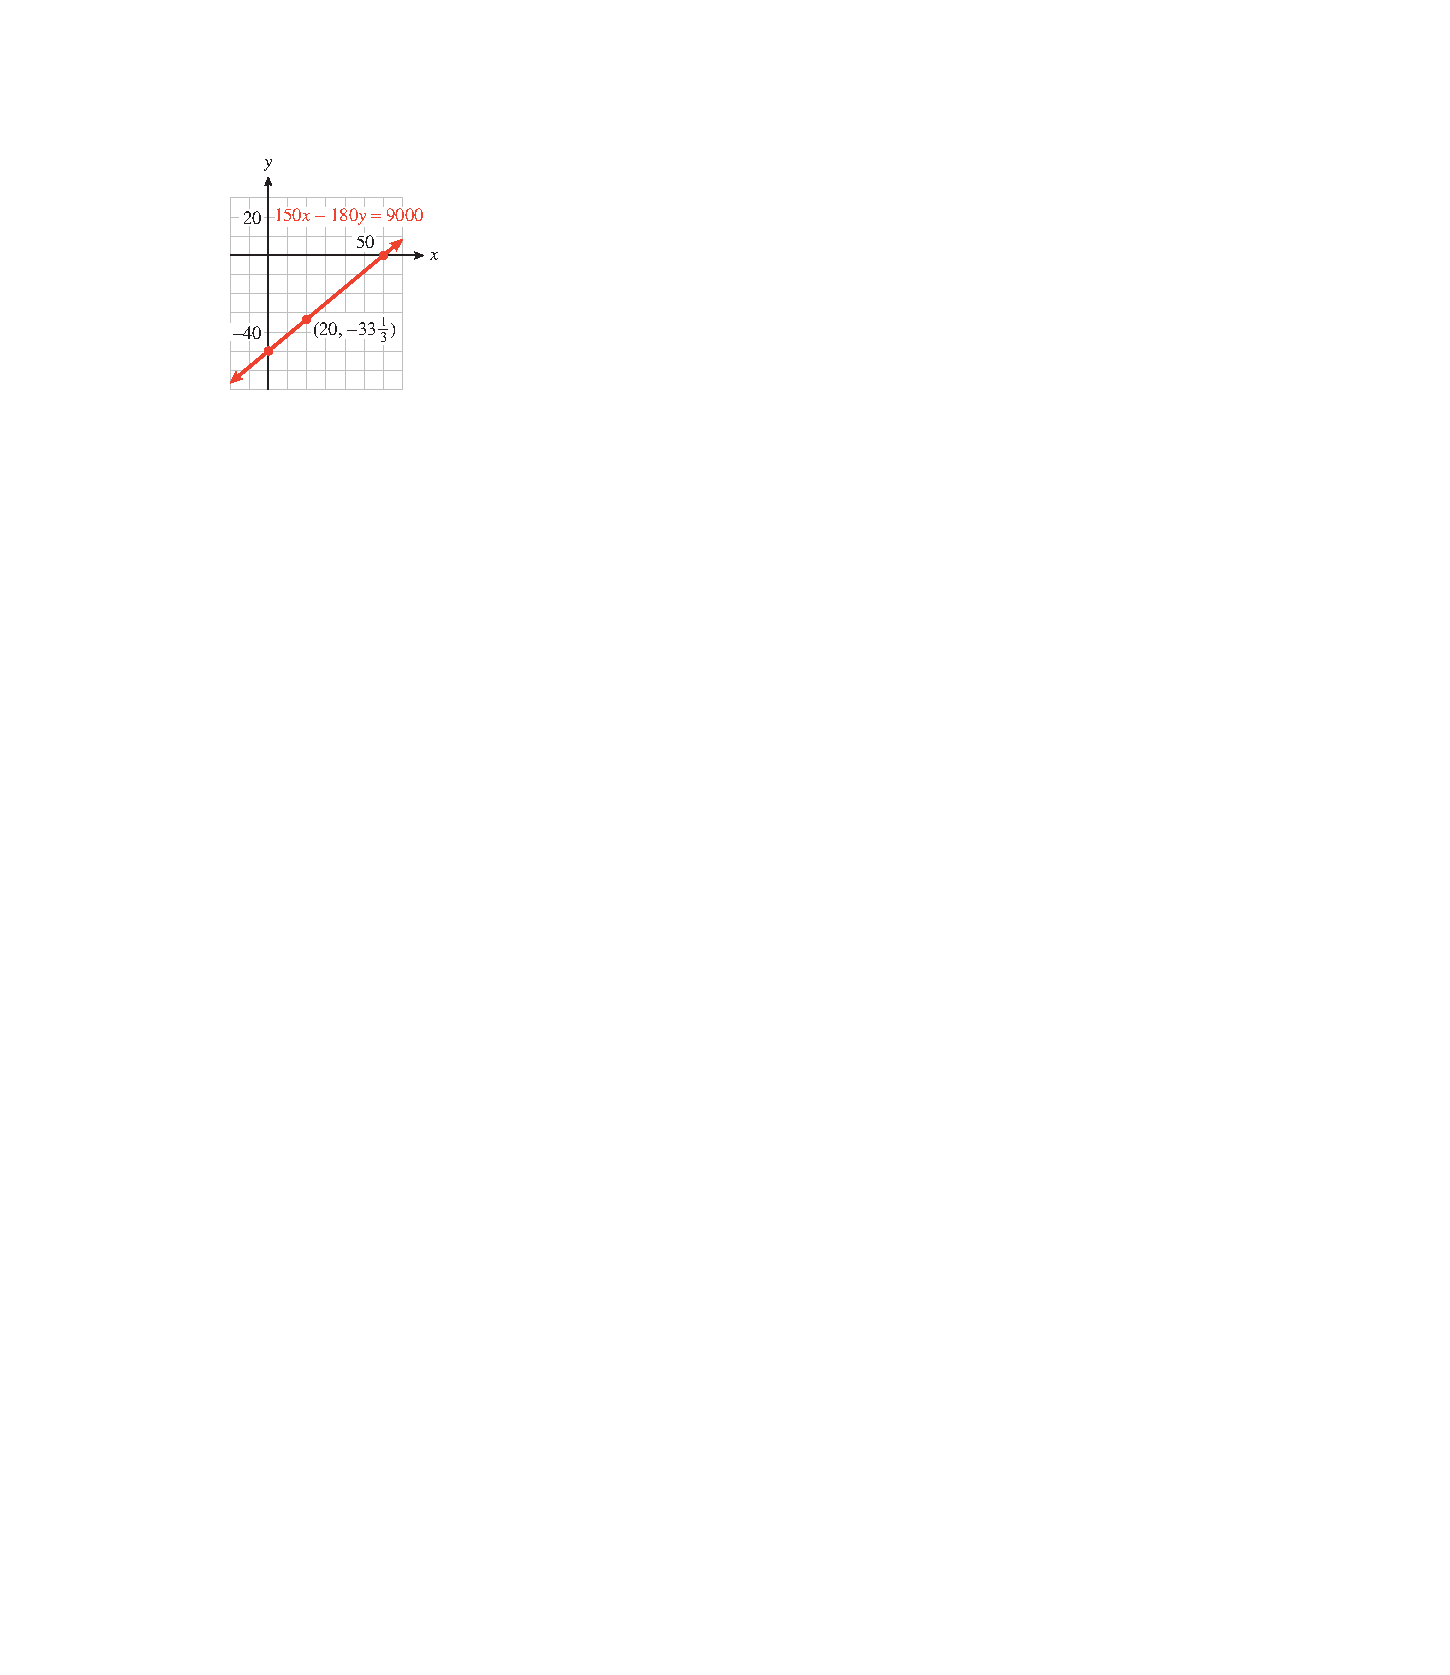
\includegraphics[width=0.5\linewidth]{images/fig-example-graph-intercepts}
\caption{\label{fig-example-graph-intercepts}}
\end{figure}
%
\end{enumerate}
\end{example}
\begin{remark}[Choosing a Graphing Window]\label{remark-2}
Knowing the intercepts can also help us choose a suitable window on a graphing calculator. We would like the window to be large enough to show the intercepts. For the graph in \hyperref[fig-example-graph-intercepts]{Figure~\ref{fig-example-graph-intercepts}}, we can enter the equation%
\begin{equation*}
Y = (9000 -150X)/ -180
\end{equation*}
in the window \begin{table}
\centering
\begin{tabular}{lll}
Xmin\(=-20\)&&Xmax\(=70\)\tabularnewline[0pt]
Ymin\(=-70\)&&Ymax\(=30\)
\end{tabular}
\end{table}
%
\end{remark}
\begin{assemblage}{To Graph a Line Using the Intercept Method:}\label{assemblage-3}
\leavevmode%
\begin{enumerate}[label=*\arabic**]
\item\hypertarget{li-67}{}Find the intercepts of the line.%
%
\begin{enumerate}[label=++\alph*]
\item\hypertarget{li-68}{}To find the \(x\)-intercept, set \(y=0\) and solve for \(x\).%
\item\hypertarget{li-69}{}To find the \(y\)-intercept, set \(x = 0\) and solve for \(y\).%
\end{enumerate}
\item\hypertarget{li-70}{}Plot the intercepts.%
\item\hypertarget{li-71}{}Choose a value for \(x\) and find a third point on the line.%
\item\hypertarget{li-72}{}Draw a line through the points.%
\end{enumerate}
%
\end{assemblage}
\begin{exercise}\label{exercise-intercepts}
\leavevmode%
\begin{enumerate}[label=\alph*]
\item\hypertarget{li-73}{}In \hyperref[exercise-crops]{Exercise~\ref{exercise-crops}}, you wrote an equation about crops in Nebraska. Find the intercepts of the graph.%
\item\hypertarget{li-74}{}Use the intercepts to help you choose appropriate scales for the axes, and then graph the equation.%
\item\hypertarget{li-75}{}What do the intercepts tell us about the problem?%
\end{enumerate}
\end{exercise}
The examples in this section model simple linear relationships between two variables. Such relationships, in which the value of one variable is determined by the value of the other, are called \terminology{functions}. We will study various kinds of functions throughout the course.%
\typeout{************************************************}
\typeout{Subsection 1.1.6 Section Summary}
\typeout{************************************************}
\subsection[{Section Summary}]{Section Summary}\label{summary-1-1}
\typeout{************************************************}
\typeout{Subsubsection 1.1.6.1 Vocabulary}
\typeout{************************************************}
\subsubsection[{Vocabulary}]{Vocabulary}\label{subsubsection-1}
Look up the definitions of new terms in the Glossary. \leavevmode%
\begin{multicols}{3}
\begin{itemize}[label=\textbullet]
\item{}Variable%
\item{}Mathematical model%
\item{}Increasing graph%
\item{}Linear equation%
\item{}Solve an equation%
\item{}Evaluate an expression%
\item{}Intercept%
\item{}Decreasing graph%
\end{itemize}
\end{multicols}
%
\typeout{************************************************}
\typeout{Subsubsection 1.1.6.2 CONCEPTS}
\typeout{************************************************}
\subsubsection[{CONCEPTS}]{CONCEPTS}\label{subsubsection-2}
\leavevmode%
\begin{enumerate}[label=\arabic*]
\item\hypertarget{li-84}{}We can describe a relationship between variables with a table of values, a graph, or an equation.%
\item\hypertarget{li-85}{}Linear models have equations of the following form:%
\begin{equation*}
y = (\text{starting value}) + (\text{rate of change})\cdot x
\end{equation*}
%
\item\hypertarget{li-86}{}To make a useful graph, we must choose appropriate scales for the axes.%
\item\hypertarget{li-87}{}\begin{assemblage}{General Form for a Linear Equation}\label{assemblage-4}
The graph of any equation%
\begin{equation*}
Ax+By=C
\end{equation*}
where \(A\) and \(B\) are not both equal to zero, is a straight line.%
\end{assemblage}
%
\item\hypertarget{li-88}{}The intercepts of a graph are the points where the graph crosses the axes.%
\item\hypertarget{li-89}{}We can use the intercepts to graph a line.%
\begin{assemblage}{To Graph a Line Using the Intercept Method:}\label{assemblage-5}
%
\begin{enumerate}[label=\arabic*]
\item\hypertarget{li-90}{}Find the intercepts of the line.%
%
\begin{enumerate}[label=++\alph*]
\item\hypertarget{li-91}{}To find the \(x\)-intercept, set \(y=0\) and solve for \(x\).%
\item\hypertarget{li-92}{}To find the \(y\)-intercept, set \(x = 0\) and solve for \(y\).%
\end{enumerate}
\item\hypertarget{li-93}{}Plot the intercepts.%
\item\hypertarget{li-94}{}Choose a value for \(x\) and find a third point on the line.%
\item\hypertarget{li-95}{}Draw a line through the points.%
\end{enumerate}
%
\end{assemblage}
\item\hypertarget{li-96}{}The intercepts are also useful for interpreting a model.%
\end{enumerate}
%
\typeout{************************************************}
\typeout{Subsubsection 1.1.6.3 STUDY QUESTIONS}
\typeout{************************************************}
\subsubsection[{STUDY QUESTIONS}]{STUDY QUESTIONS}\label{subsubsection-3}
\leavevmode%
\begin{enumerate}[label=\arabic*]
\item\hypertarget{li-97}{}Name three ways to represent a relationship between two variables.%
\item\hypertarget{li-98}{}If \(C\) is expressed in terms of \(H\), which variable goes on the horizontal axis?%
\item\hypertarget{li-99}{}Explain the difference between evaluating an expression and solving an equation.%
\item\hypertarget{li-100}{}How many points do you need to graph a linear equation?%
\item\hypertarget{li-101}{}Explain how the words \terminology{intercept} and \terminology{intersect} are related; explain how they are different.%
\item\hypertarget{li-102}{}Delbert says that the intercepts of the line \(3x + 5y = 30\) are \((10, 6)\). What is wrong with his answer?%
\end{enumerate}
%
\typeout{************************************************}
\typeout{Subsubsection 1.1.6.4 SKILLS}
\typeout{************************************************}
\subsubsection[{SKILLS}]{SKILLS}\label{subsubsection-4}
Practice each skill in the \hyperref[section-1-1-exercises]{Homework~\ref{section-1-1-exercises}} problems listed. \leavevmode%
\begin{enumerate}[label=\arabic*]
\item\hypertarget{li-103}{}Make a table of values: \#1\textendash{}4, 7 and 8%
\item\hypertarget{li-104}{}Plot points and draw a graph: \#1– 4, 7 and 8%
\item\hypertarget{li-105}{}Choose appropriate scales for the axes: \#5\textendash{}12%
\item\hypertarget{li-106}{}Write a linear model of the form \(y = (\text{starting value}) + (\text{rate of change})\cdot x\): \#1\textendash{}8%
\item\hypertarget{li-107}{}Write a linear model in general form: \#25\textendash{}28, 33\textendash{}36%
\item\hypertarget{li-108}{}Evaluate a linear expression, algebraically and graphically: \#1\textendash{}4%
\item\hypertarget{li-109}{}Solve a linear equation, algebraically and graphically: \#1\textendash{}4%
\item\hypertarget{li-110}{}Find the intercepts of a graph: \#5 and 6, 13–24, 45–52%
\item\hypertarget{li-111}{}Graph a line by the intercept method: \#5 and 6, 13–24%
\item\hypertarget{li-112}{}Interpret the meaning of the intercepts: \#5 and 6, 25–28%
\item\hypertarget{li-113}{}Use a graphing calculator to graph a line: \#37\textendash{}52%
\item\hypertarget{li-114}{}Sketch on paper a graph obtained on a calculator: \#37\textendash{}44%
\end{enumerate}
%
\typeout{************************************************}
\typeout{Exercises 1.1.7 Homework}
\typeout{************************************************}
\subsection[{Homework}]{Homework}\label{section-1-1-exercises}
\begin{exerciselist}
\item[1.]\hypertarget{exercise-8}{}The temperature in the desert at 6 a.m., just before sunrise, was \(65\degree\)F. The temperature rose \(5\) degrees every hour until it reached its maximum value at about 5 p.m. Complete the table of values for the temperature, \(T\), at \(h\) hours after 6 a.m. \begin{table}
\centering
\begin{tabular}{AcAcAcAcAcAcA}\hrulethick
\(h\)&\(0\)&\(3\)&\(6\)&\(9\)&\(10\)\tabularnewline\hrulethin
\(T\)&\(\hphantom{0000}\)&\(\hphantom{0000}\)&\(\hphantom{0000}\)&\(\hphantom{0000}\)&\(\hphantom{0000}\)\tabularnewline\hrulethin
\end{tabular}
\end{table}
 \leavevmode%
\begin{enumerate}[label=\alph*]
\item\hypertarget{li-115}{}Write an equation for the temperature, \(T\), in terms of \(h\).%
\item\hypertarget{li-116}{}Graph the equation. 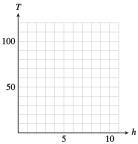
\includegraphics[width=0.5\linewidth]{images/fig-ex-1-1-1}
%
\item\hypertarget{li-117}{}How hot is it at noon? Illustrate the answer on your graph.%
\item\hypertarget{li-118}{}When will the temperature be \(110\degree\)F? Illustrate the answer on your graph.%
\end{enumerate}
%
\par\smallskip
\par\smallskip
\noindent\textbf{Answer.}\hypertarget{answer-8}{}\quad
\begin{tabular}{AcAcAcAcAcAcA}\hrulethick
\(h\)&\(0\)&\(3\)&\(6\)&\(9\)&\(10\)\tabularnewline\hrulethin
\(T\)&\(65\)&\(80\)&\(95\)&\(110\)&\(115\)\tabularnewline\hrulethin
\end{tabular}
 \leavevmode%
\begin{enumerate}[label=\alph*]
\item\hypertarget{li-119}{}\(T=65+5h\)%
\item\hypertarget{li-120}{}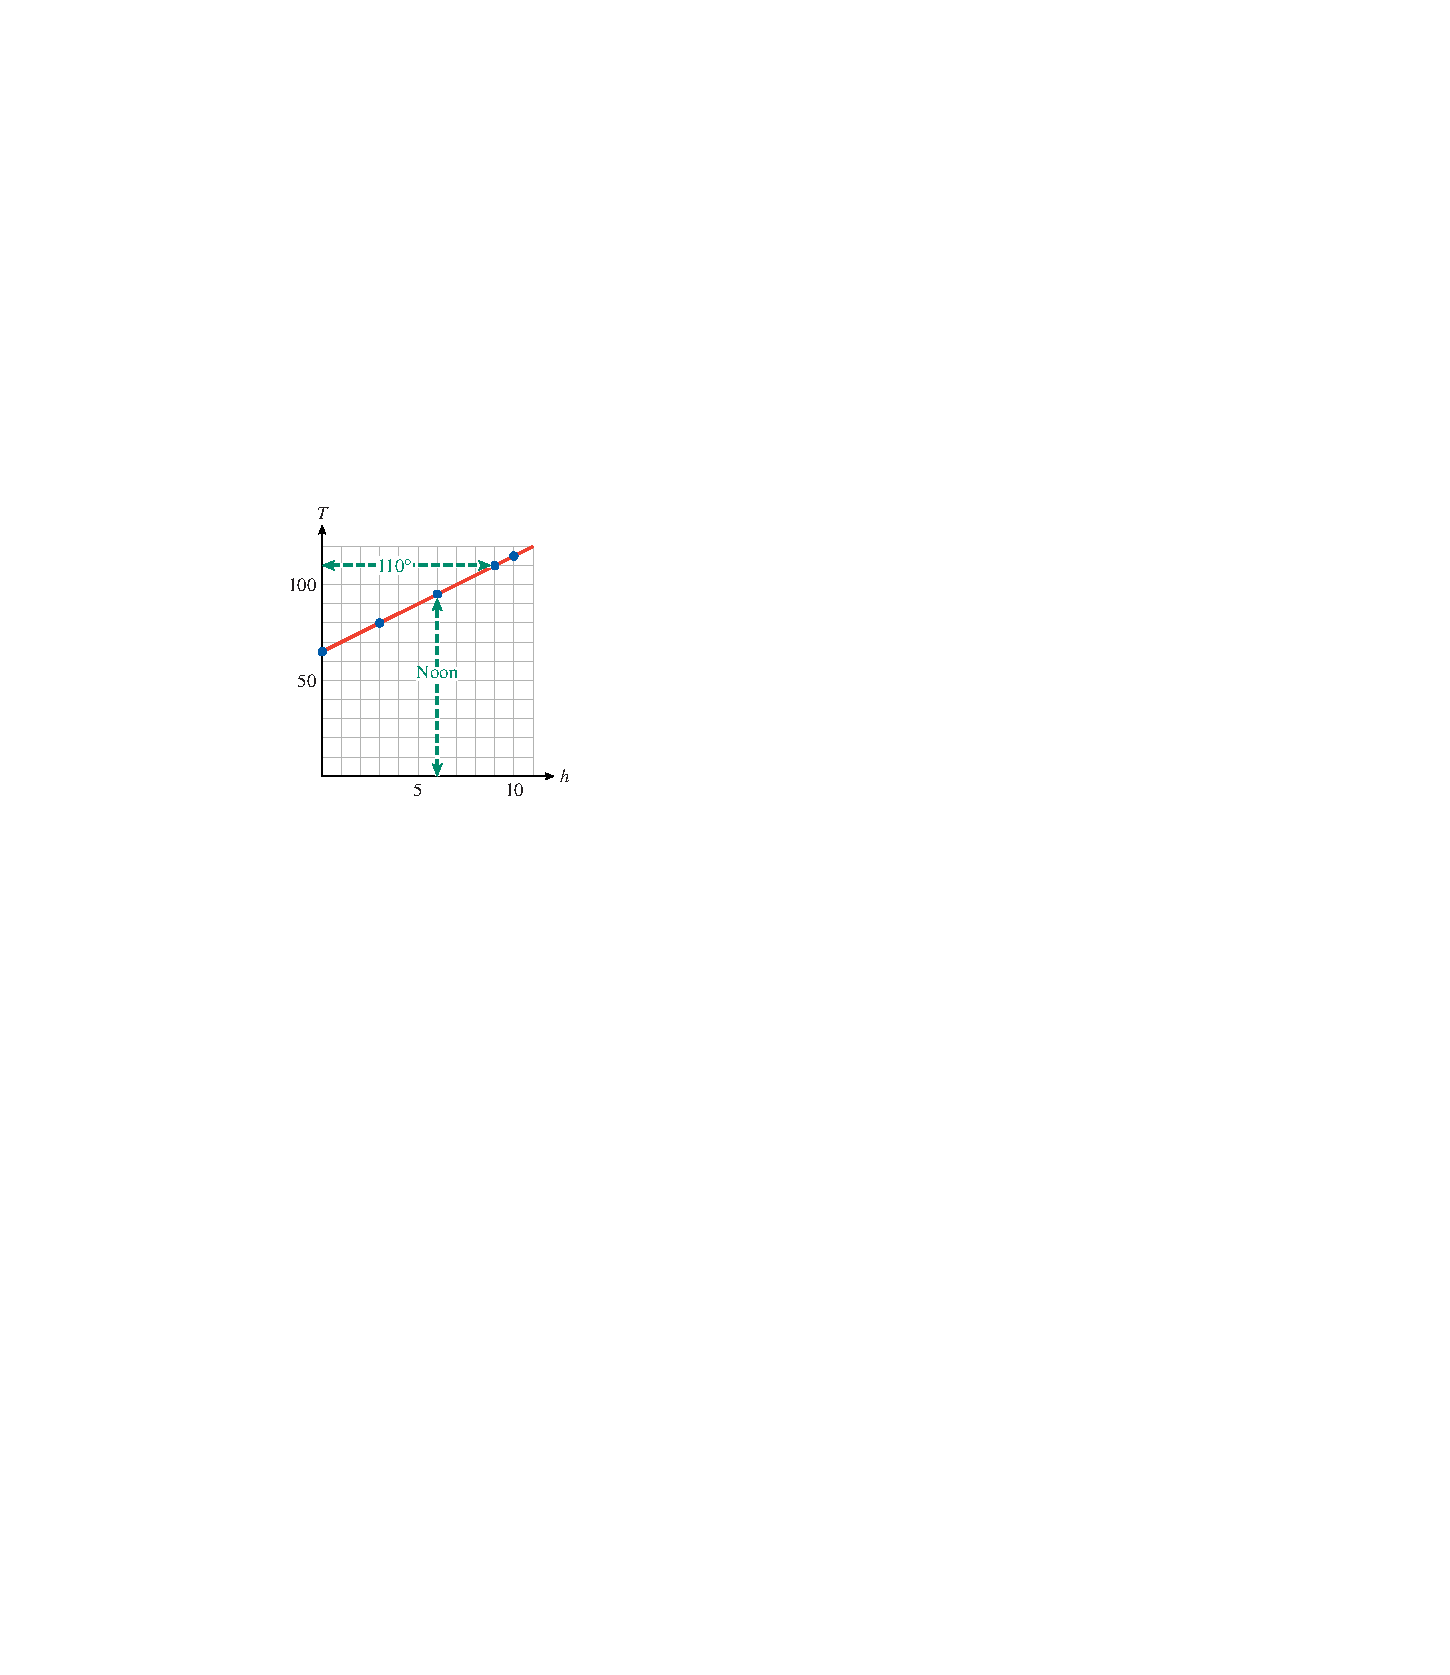
\includegraphics[width=0.5\linewidth]{images/fig-ans-1-1-1}
%
\item\hypertarget{li-121}{}\(95\degree\)%
\item\hypertarget{li-122}{}3 p.m.%
\end{enumerate}
%
\item[2.]\hypertarget{exercise-9}{}The taxi out of Dulles Airport charges a traveler with one suitcase an initial fee of \(\$2.00\), plus \(\$1.50\) for each mile traveled. Complete the table of values showing the charge, \(C\), for a trip of \(n\) miles. \begin{table}
\centering
\begin{tabular}{AcAcAcAcAcAcAcA}\hrulethick
\(n\)&\(0\)&\(5\)&\(10\)&\(15\)&\(20\)&\(25\)\tabularnewline\hrulethin
\(C\)&\(\hphantom{0000}\)&\(\hphantom{0000}\)&\(\hphantom{0000}\)&\(\hphantom{0000}\)&\(\hphantom{0000}\)&\(\hphantom{0000}\)\tabularnewline\hrulethin
\end{tabular}
\end{table}
 \leavevmode%
\begin{enumerate}[label=(\alph*)]
\item\hypertarget{li-123}{}Write an equation for the charge, \(C\), in terms of the number of miles traveled, \(n\).%
\item\hypertarget{li-124}{}Graph the equation. 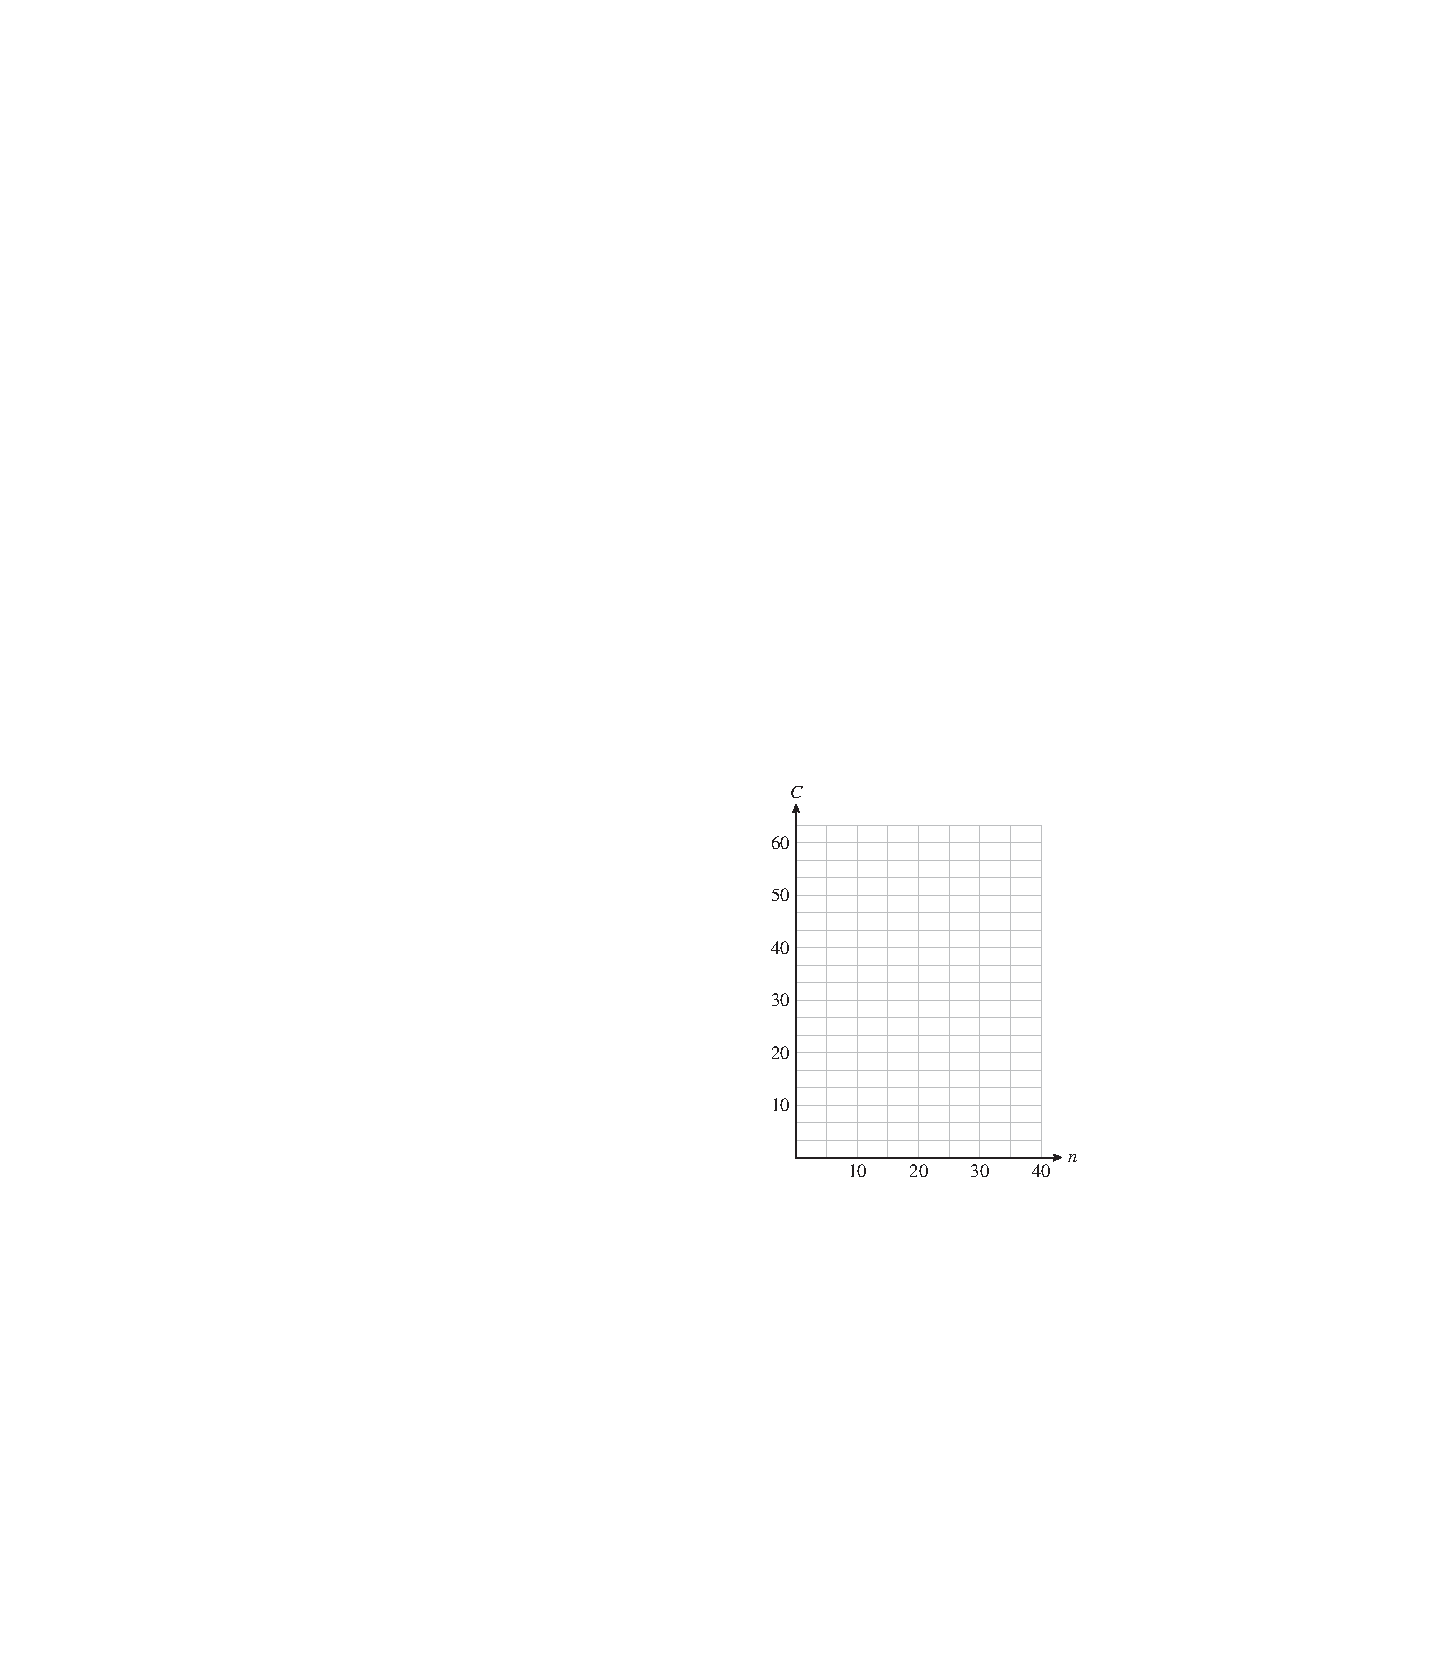
\includegraphics[width=0.5\linewidth]{images/fig-ex-1-1-2}
%
\item\hypertarget{li-125}{}What is the charge for a trip to Mount Vernon,  \(40\) miles from the airport? Illustrate the answer on your graph.%
\item\hypertarget{li-126}{}If a ride to the National Institutes of Health (NIH) costs \(\$39.50\), how far is it from the airport to the NIH? Illustrate the answer on your graph.%
\end{enumerate}
%
\par\smallskip
\item[3.]\hypertarget{exercise-10}{}On October 31, Betty and Paul fill their \(250\)-gallon oil tank for their heater. Beginning in November, they use an average of \(15\) gallons of oil per week. Complete the table of values for the amount of oil, \(A\), left in the tank after \(w\) weeks. \begin{table}
\centering
\begin{tabular}{AcAcAcAcAcAcA}\hrulethick
\(w\)&\(0\)&\(4\)&\(8\)&\(12\)&\(16\)\tabularnewline\hrulethin
\(A\)&\(\hphantom{0000}\)&\(\hphantom{0000}\)&\(\hphantom{0000}\)&\(\hphantom{0000}\)&\(\hphantom{0000}\)\tabularnewline\hrulethin
\end{tabular}
\end{table}
 \leavevmode%
\begin{enumerate}[label=(\alph*)]
\item\hypertarget{li-127}{}Write an equation that expresses the amount of oil, \(A\), in the tank in terms of the number of weeks, \(w\), since October 31.%
\item\hypertarget{li-128}{}Graph the equation. 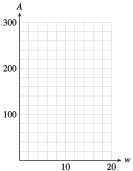
\includegraphics[width=0.5\linewidth]{images/fig-ex-1-1-3}
%
\item\hypertarget{li-129}{}How much did the amount of fuel oil in the tank decrease between the third week and the eighth week? Illustrate this amount on the graph.%
\item\hypertarget{li-130}{}When will the tank contain more than \(175\) gallons of fuel oil? Illustrate on the graph.%
\end{enumerate}
%
\par\smallskip
\par\smallskip
\noindent\textbf{Answer.}\hypertarget{answer-9}{}\quad
\begin{tabular}{AcAcAcAcAcAcA}\hrulethick
\(w\)&\(0\)&\(4\)&\(8\)&\(12\)&\(16\)\tabularnewline\hrulethin
\(A\)&\(250\)&\(190\)&\(130\)&\(70\)&\(10\)\tabularnewline\hrulethin
\end{tabular}
 \leavevmode%
\begin{enumerate}[label=(\alph*)]
\item\hypertarget{li-131}{}\(A=250-15w\)%
\item\hypertarget{li-132}{}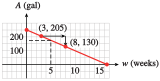
\includegraphics[width=0.5\linewidth]{images/fig-ans-1-1-3}
%
\item\hypertarget{li-133}{}75 gallons%
\item\hypertarget{li-134}{}Until the fifth week%
\end{enumerate}
%
\item[4.]\hypertarget{exercise-11}{}Leon's camper has a \(20\)-gallon gas tank, and he gets \(12\) miles to the gallon. (That is, he uses \(1⁄12\) gallon per mile.) Complete the table of values for the amount of gas, \(g\), left in Leon's tank after driving \(m\) miles. \begin{table}
\centering
\begin{tabular}{AcAcAcAcAcAcA}\hrulethick
\(m\)&\(0\)&\(48\)&\(96\)&\(144\)&\(192\)\tabularnewline\hrulethin
\(g\)&\(\hphantom{0000}\)&\(\hphantom{0000}\)&\(\hphantom{0000}\)&\(\hphantom{0000}\)&\(\hphantom{0000}\)\tabularnewline\hrulethin
\end{tabular}
\end{table}
 \leavevmode%
\begin{enumerate}[label=(\alph*)]
\item\hypertarget{li-135}{}Write an equation that expresses the amount of gas, \(g\), in Leon's fuel tank in terms of the number of miles, \(m\), he has driven.%
\item\hypertarget{li-136}{}Graph the equation. 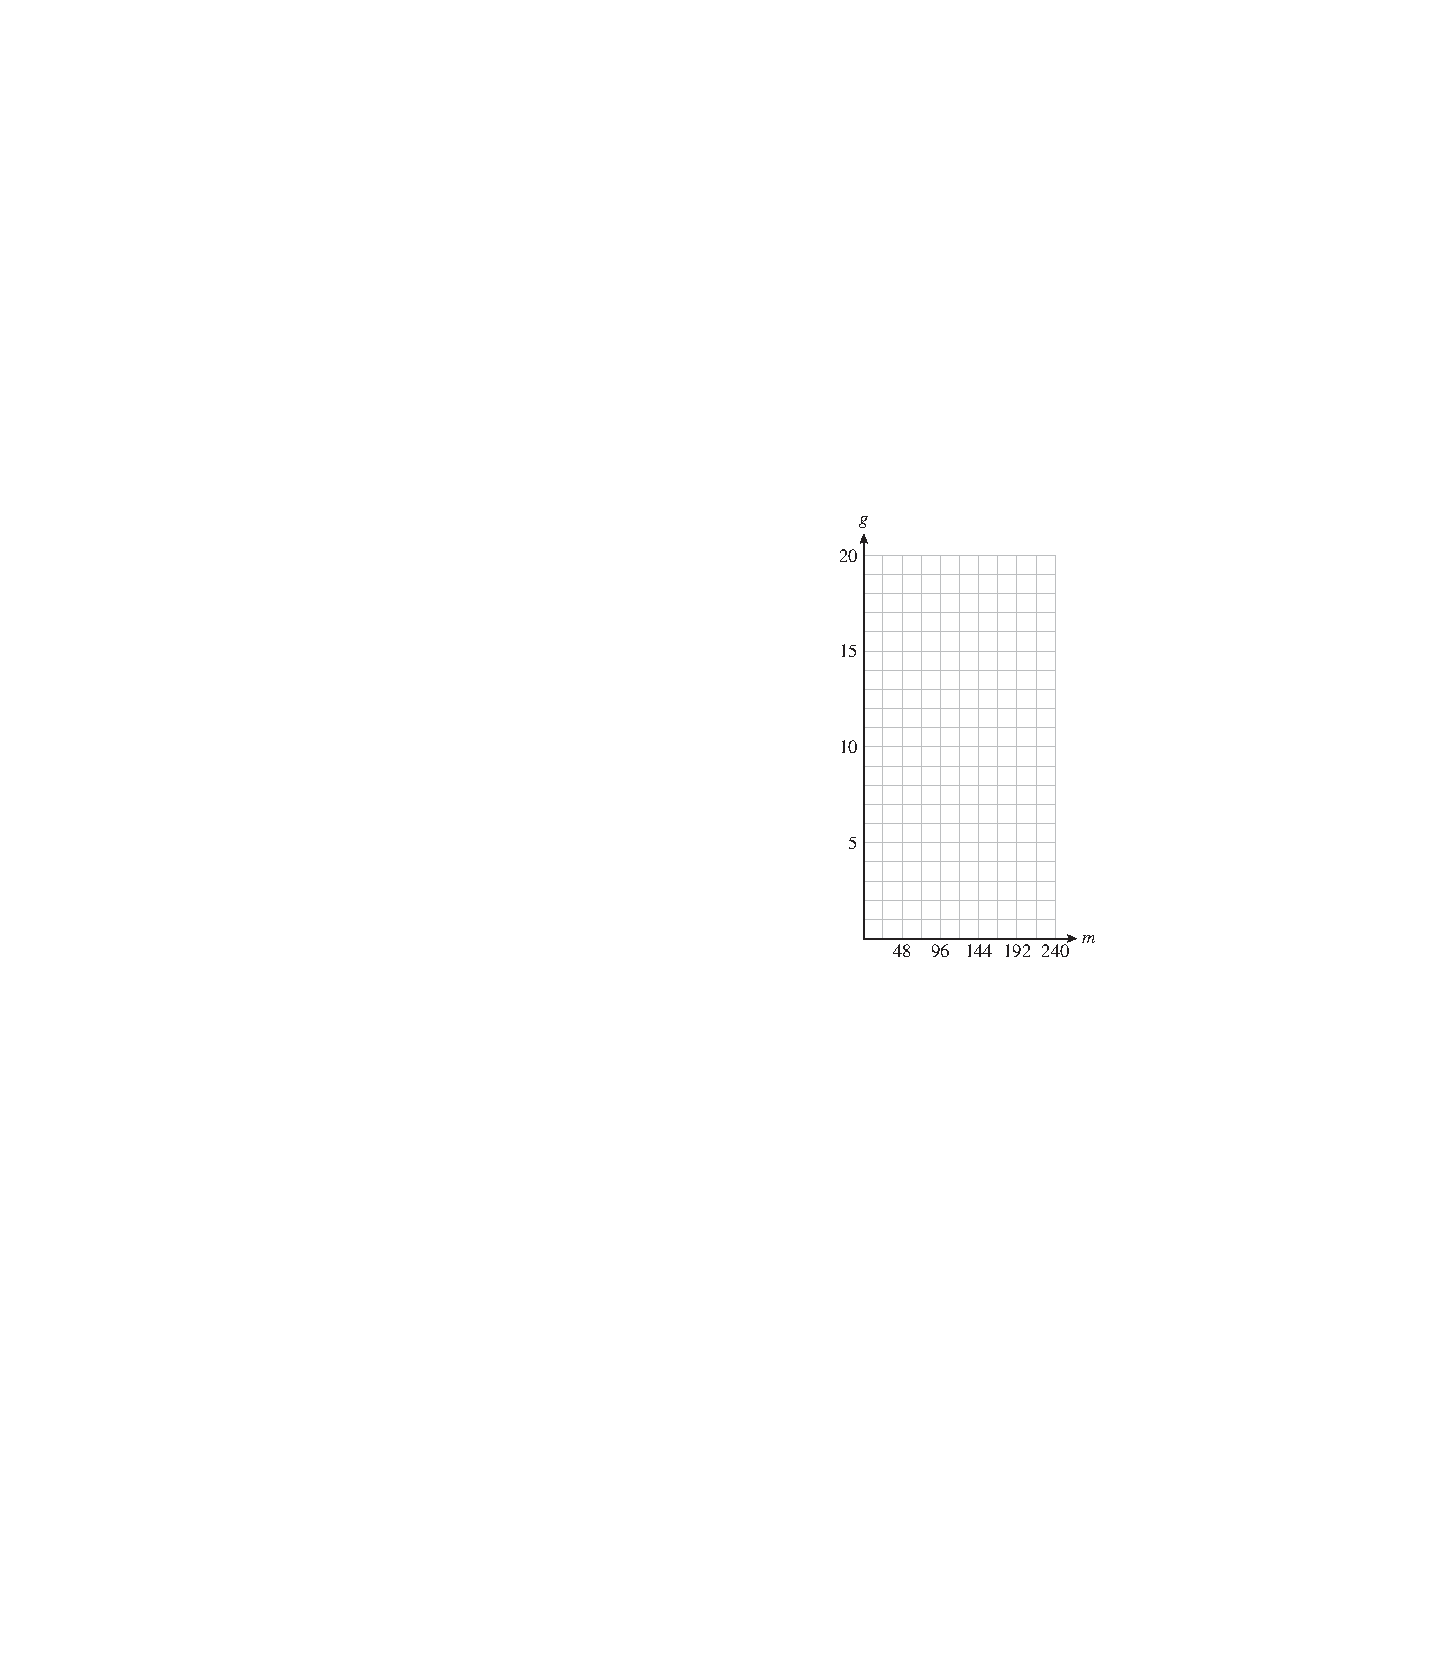
\includegraphics[width=0.5\linewidth]{images/fig-ex-1-1-4}
%
\item\hypertarget{li-137}{}How much gas will Leon use between 8 a.m., when his odometer reads \(96\) miles, and 9 a.m., when the odometer reads \(144\) miles? Illustrate on the graph.%
\item\hypertarget{li-138}{}If Leon has less than \(5\) gallons of gas left, how many miles has he driven? Illustrate on the graph.%
\end{enumerate}
%
\par\smallskip
\item[5.]\hypertarget{exercise-12}{}Phil and Ernie buy a used photocopier for \(\$800\) and set up a copy service on their campus. For each hour that the copier runs, Phil and Ernie make \(\$40\). \leavevmode%
\begin{enumerate}[label=(\alph*)]
\item\hypertarget{li-139}{}Write an equation that expresses Phil and Ernie's profit (or loss), \(P\), in terms of the number of hours, \(t\), they run the copier.%
\item\hypertarget{li-140}{}Find the intercepts and sketch the graph. (Suggestion: Scale the horizontal axis from \(0\) to \(40\) in increments of \(5\), and scale the vertical axis from \(-1000\) to \(400\) in increments of \(100\).)%
\item\hypertarget{li-141}{}What do the intercepts tell us about the profit?%
\end{enumerate}
%
\par\smallskip
\par\smallskip
\noindent\textbf{Answer.}\hypertarget{answer-10}{}\quad
\leavevmode%
\begin{enumerate}[label=(\alph*)]
\item\hypertarget{li-142}{}\(P=-800+40t\)%
\item\hypertarget{li-143}{}\((0,-800)\), \((20,0)\) 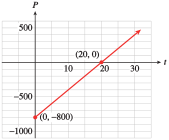
\includegraphics[width=0.5\linewidth]{images/fig-ans-1-1-5}
%
\item\hypertarget{li-144}{}The \(P\)-intercept, \(800\), is the initial \((t = 0)\) value of the profit. Phil and Ernie start out \(\$800\) in debt. The \(t\)-intercept, \(20\), is the number of hours required for Phil and Ernie to break even.%
\end{enumerate}
%
\item[6.]\hypertarget{exercise-13}{}A deep-sea diver is taking some readings at a depth of \(400\) feet. He begins rising at \(20\) feet per minute. \leavevmode%
\begin{enumerate}[label=(\alph*)]
\item\hypertarget{li-145}{}Write an equation that expresses the diver’s altitude, \(h\), in terms of the number of minutes, \(m\), elapsed. (Consider a depth of \(400\) feet as an altitude of \(-400\) feet.)%
\item\hypertarget{li-146}{}Find the intercepts and sketch the graph. (Suggestion: Scale the horizontal axis from \(0\) to \(24\) in increments of \(2\), and scale the vertical axis from \(-500\) to \(100\) in increments of \(50\).)%
\item\hypertarget{li-147}{}What do the intercepts tell us about the diver's depth?%
\end{enumerate}
%
\par\smallskip
\item[7.]\hypertarget{exercise-14}{}There are many formulas for estimating the annual cost of driving. The Automobile Club estimates that fixed costs for a small car—including insurance, registration, depreciation, and financing—total about \(\$5000\) per year. The operating costs for gasoline, oil, maintenance, tires, and so forth are about \(12.5\) cents per mile. (Source: Automobile Association of America) \leavevmode%
\begin{enumerate}[label=(\alph*)]
\item\hypertarget{li-148}{}Write an equation for the annual driving cost, \(C\), in terms of \(d\), the number of miles driven.%
\item\hypertarget{li-149}{}Complete the table of values. \leavevmode%
\begin{table}
\centering
\begin{tabular}{AlAcAcAcAcAcA}\hrulethick
Miles Driven&\(4000\)&\(8000\)&\(12,000\)&\(16,000\)&\(20,000\)\tabularnewline\hrulethin
Cost (\textdollar{})&\(\hphantom{0000}\)&\(\hphantom{0000}\)&\(\hphantom{0000}\)&\(\hphantom{0000}\)&\(\hphantom{0000}\)\tabularnewline\hrulethin
\end{tabular}
\end{table}
%
\item\hypertarget{li-150}{}Choose scales for the axes and graph the equation.%
\item\hypertarget{li-151}{}How much does the annual cost of driving increase when the mileage increases from \(8000\) to \(12,000\) miles? Illustrate this amount on the graph.%
\item\hypertarget{li-152}{}How much mileage will cause the annual cost to exceed \(\$7000\)? Illustrate on the graph.%
\end{enumerate}
%
\par\smallskip
\par\smallskip
\noindent\textbf{Answer.}\hypertarget{answer-11}{}\quad
\leavevmode%
\begin{enumerate}[label=(\alph*)]
\item\hypertarget{li-153}{}\(C=5000+0.125d\)%
\item\hypertarget{li-154}{}Complete the table of values. \leavevmode%
\begin{table}
\centering
\begin{tabular}{AlAcAcAcAcAcA}\hrulethick
Miles Driven&\(4000\)&\(8000\)&\(12,000\)&\(16,000\)&\(20,000\)\tabularnewline\hrulethin
Cost (\textdollar{})&\(5500\)&\(6000\)&\(6500\)&\(7000\)&\(7500\)\tabularnewline\hrulethin
\end{tabular}
\end{table}
%
\item\hypertarget{li-155}{}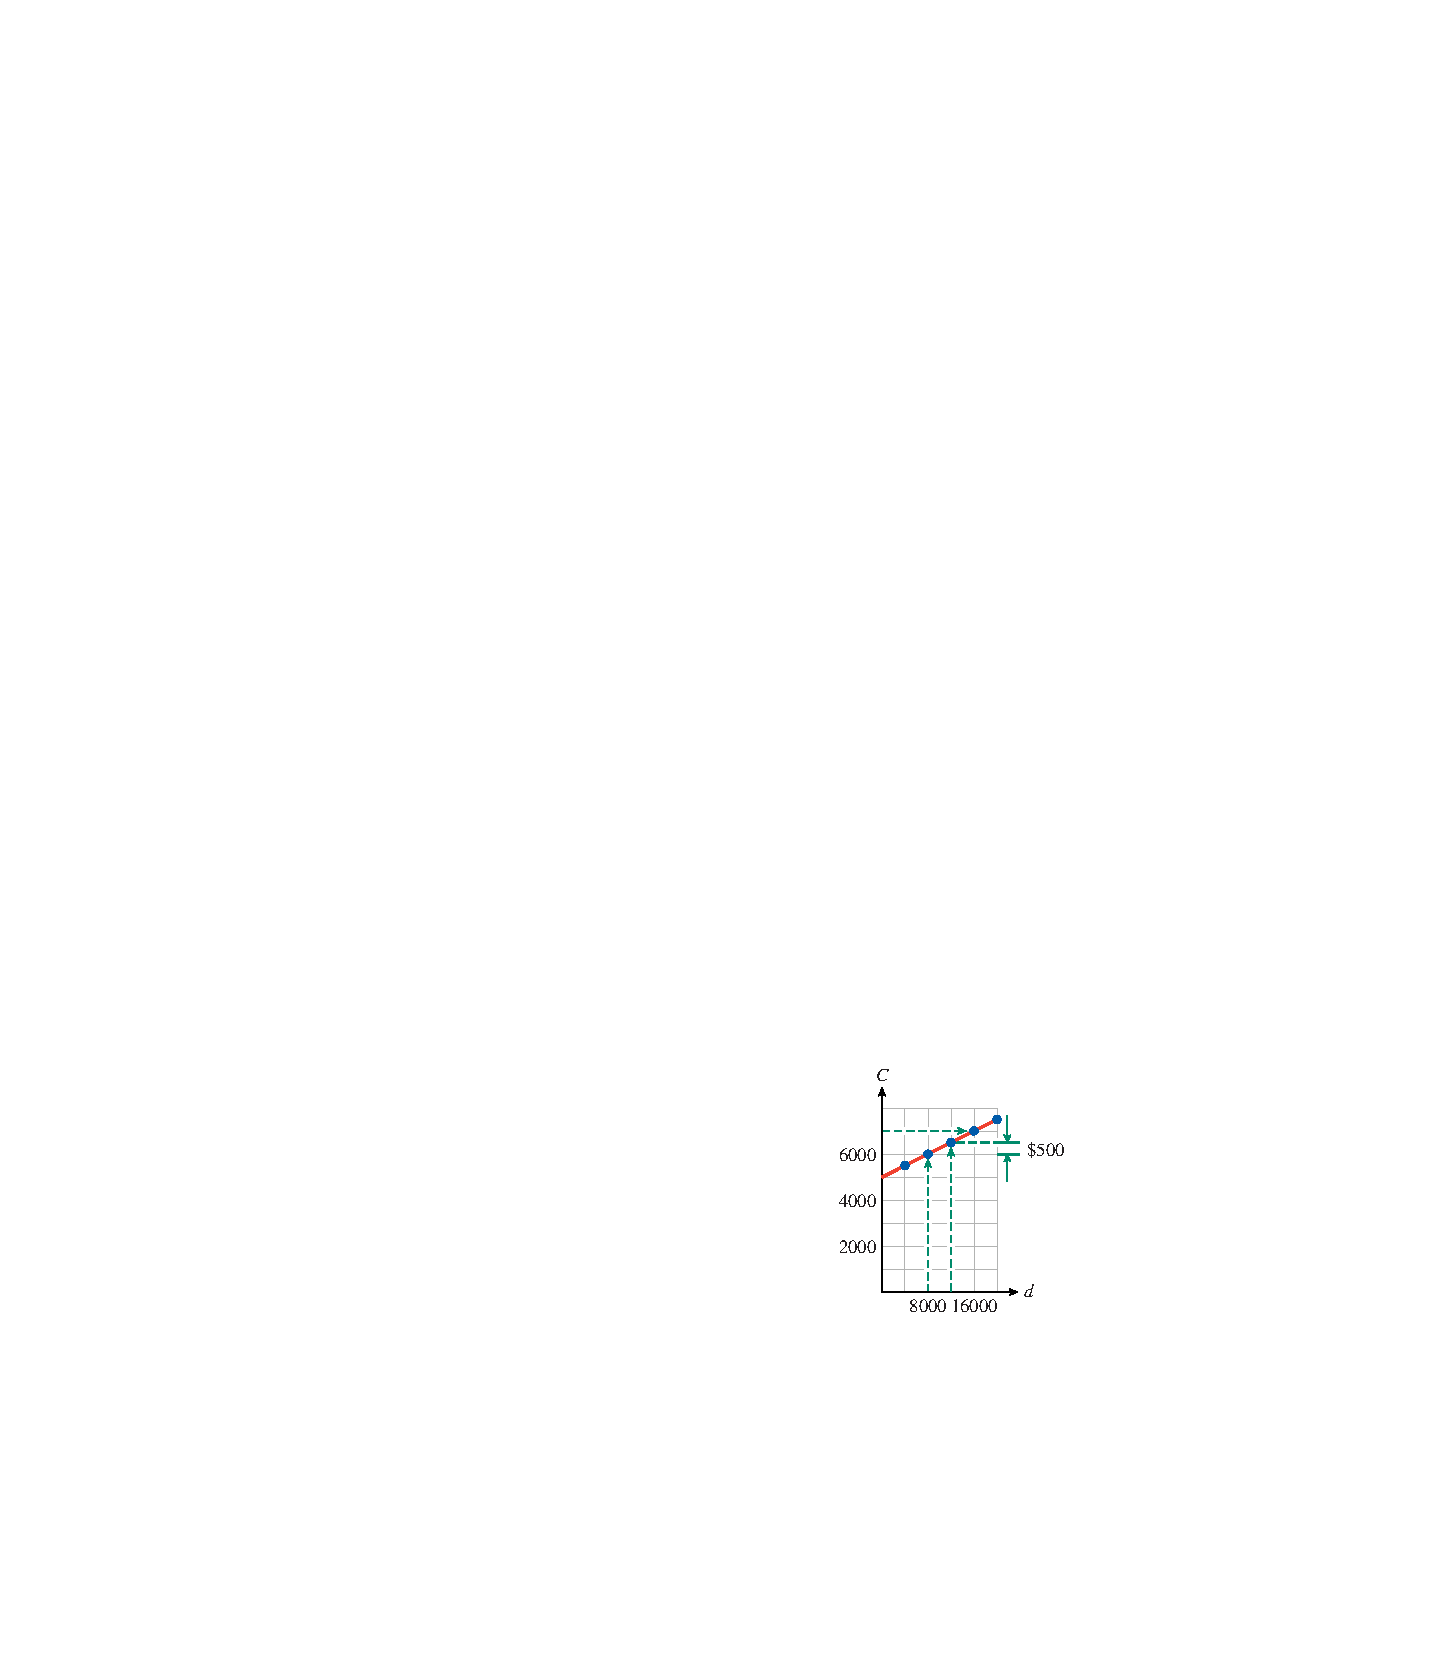
\includegraphics[width=0.5\linewidth]{images/fig-ans-1-1-7}
%
\item\hypertarget{li-156}{}\(\$500\)%
\item\hypertarget{li-157}{}More than 16,000 miles%
\end{enumerate}
%
\item[8.]\hypertarget{exercise-15}{}The boiling point of water changes with altitude. At sea level, water boils at \(212\degree\)F, and the boiling point diminishes by approximately \(0.002\degree\)F for each \(1\)-foot increase in altitude. \leavevmode%
\begin{enumerate}[label=(\alph*)]
\item\hypertarget{li-158}{}Write an equation for the boiling point, \(B\), in terms of \(a\), the altitude in feet.%
\item\hypertarget{li-159}{}Complete the table of values. \leavevmode%
\begin{table}
\centering
\begin{tabular}{AlAcAcAcAcAcAcAcA}\hrulethick
Altitude (ft)&\(-500\)&\(0\)&\(1000\)&\(2000\)&\(3000\)&\(4000\)&\(5000\)\tabularnewline\hrulethin
Boiling point (\(\degree\)F)&\(\hphantom{0000}\)&\(\hphantom{0000}\)&\(\hphantom{0000}\)&\(\hphantom{0000}\)&\(\hphantom{0000}\)&\(\hphantom{0000}\)&\(\hphantom{0000}\)\tabularnewline\hrulethin
\end{tabular}
\end{table}
%
\item\hypertarget{li-160}{}Choose scales for the axes and graph the equation.%
\item\hypertarget{li-161}{}How much does the boiling point decrease when the altitude increases from \(1000\) to \(3000\) feet? Illustrate this amount on the graph.%
\item\hypertarget{li-162}{}At what altitudes is the boiling point less than \(204\degree\)F? Illustrate on the graph.%
\end{enumerate}
%
\par\smallskip
\hypertarget{exercisegroup-1}{}\par\noindent For each table, choose appropriate scales for the axes and plot the given points.%
\begin{exercisegroup}(2)
\exercise[9.]\hypertarget{exercise-16}{}\begin{tabular}{AlAcAcAcAcA}\hrulethick
\(x\)&\(0\)&\(80\)&\(90\)&\(120\)\tabularnewline\hrulethin
\(y\)&\(6\)&\(2\)&\(1.5\)&\(1\)\tabularnewline\hrulethin
\end{tabular}
%
\par\smallskip
\noindent\textbf{Answer.}\hypertarget{answer-12}{}\quad
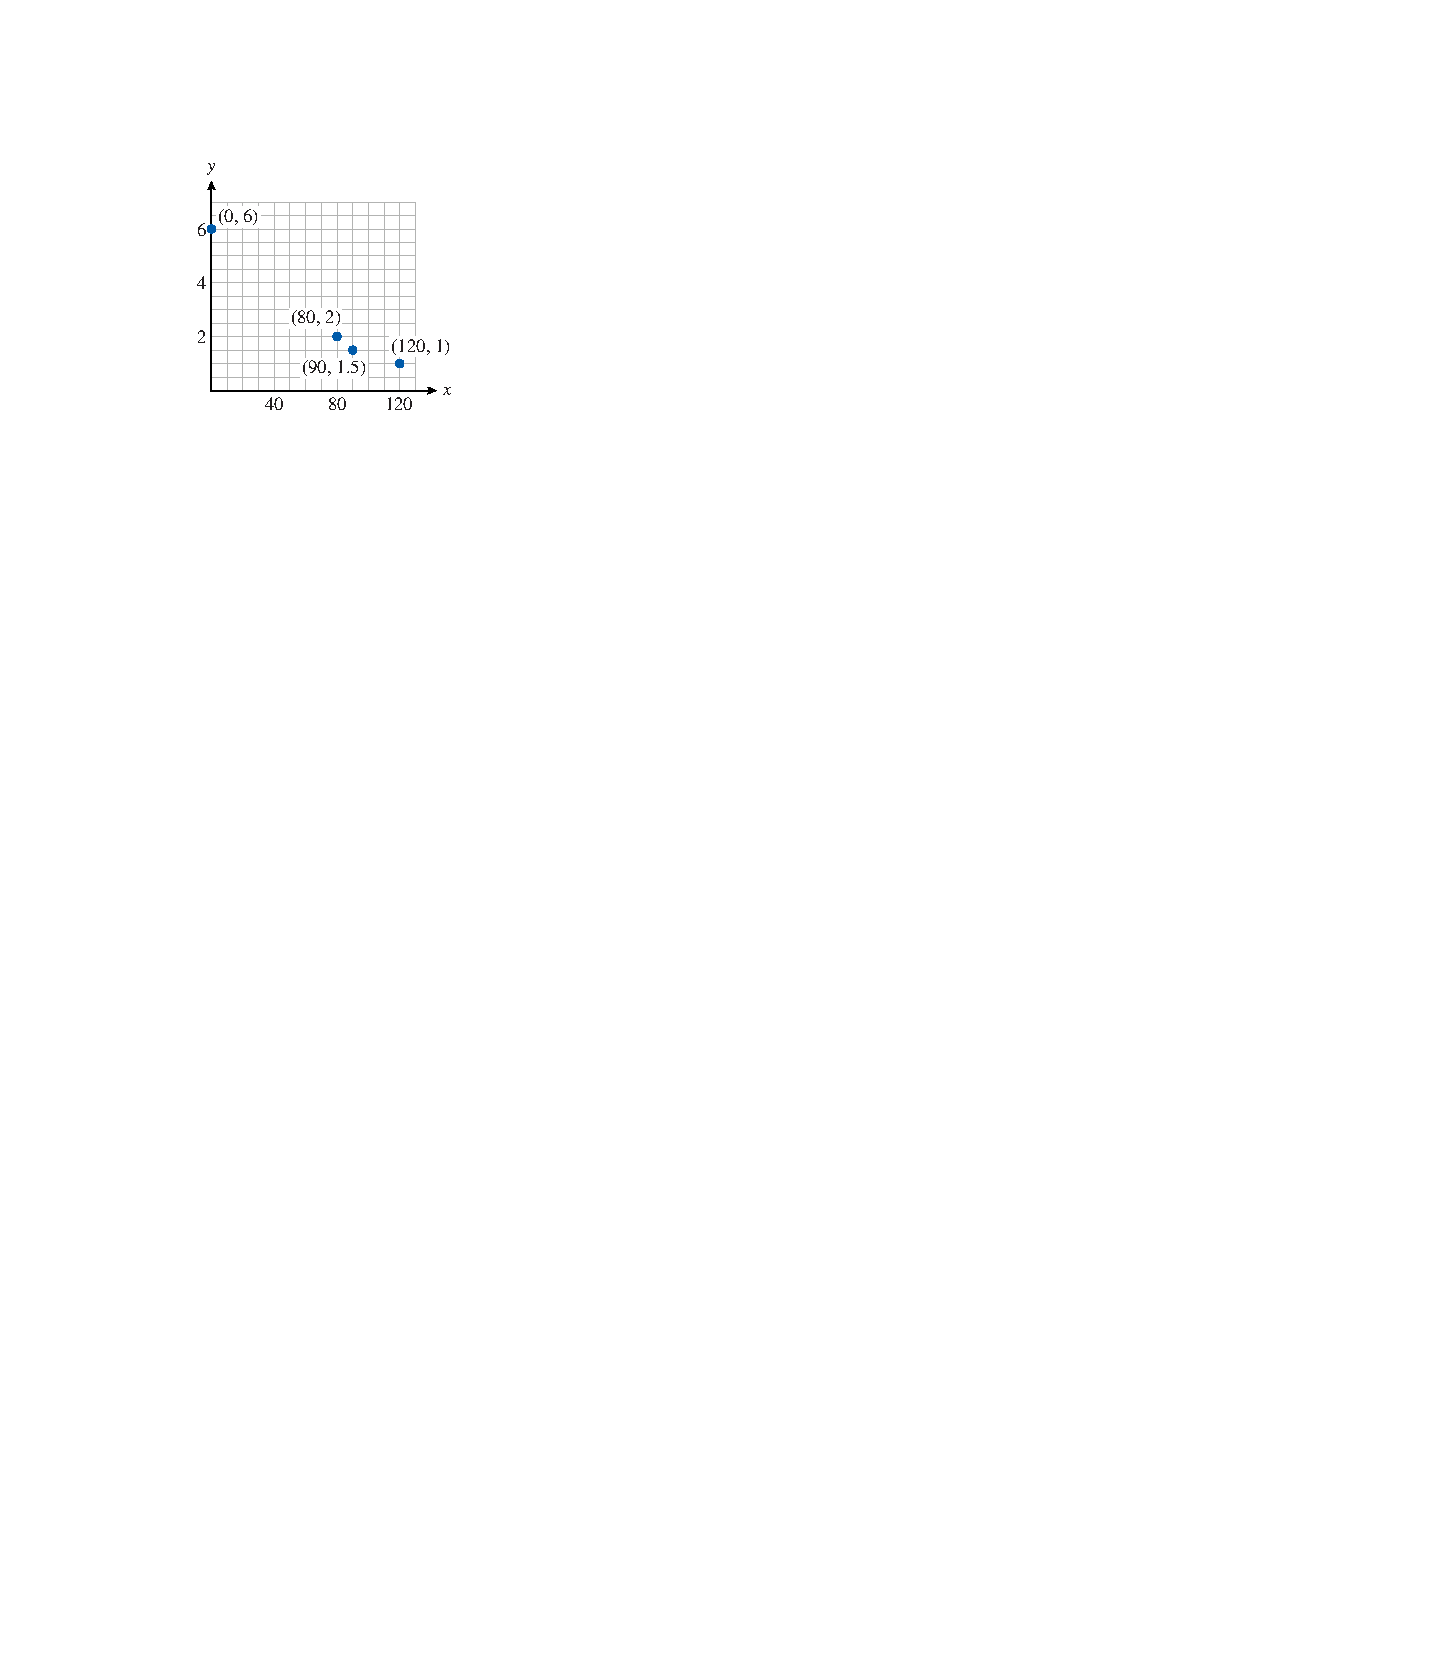
\includegraphics[width=0.5\linewidth]{images/fig-ans-1-1-9}
%
\exercise[10.]\hypertarget{exercise-17}{}\begin{tabular}{AlAcAcAcAcA}\hrulethick
\(x\)&\(300\)&\(500\)&\(800\)&\(1100\)\tabularnewline\hrulethin
\(y\)&\(1.2\)&\(1.3\)&\(1.5\)&\(1.9\)\tabularnewline\hrulethin
\end{tabular}
%
\exercise[11.]\hypertarget{exercise-18}{}\begin{tabular}{AlAcAcAcAcA}\hrulethick
\(x\)&\(0.01\)&\(0.03\)&\(0.06\)&\(0.07\)\tabularnewline\hrulethin
\(y\)&\(-0.2\)&\(-1\)&\(-1.1\)&\(-2\)\tabularnewline\hrulethin
\end{tabular}
%
\par\smallskip
\noindent\textbf{Answer.}\hypertarget{answer-13}{}\quad
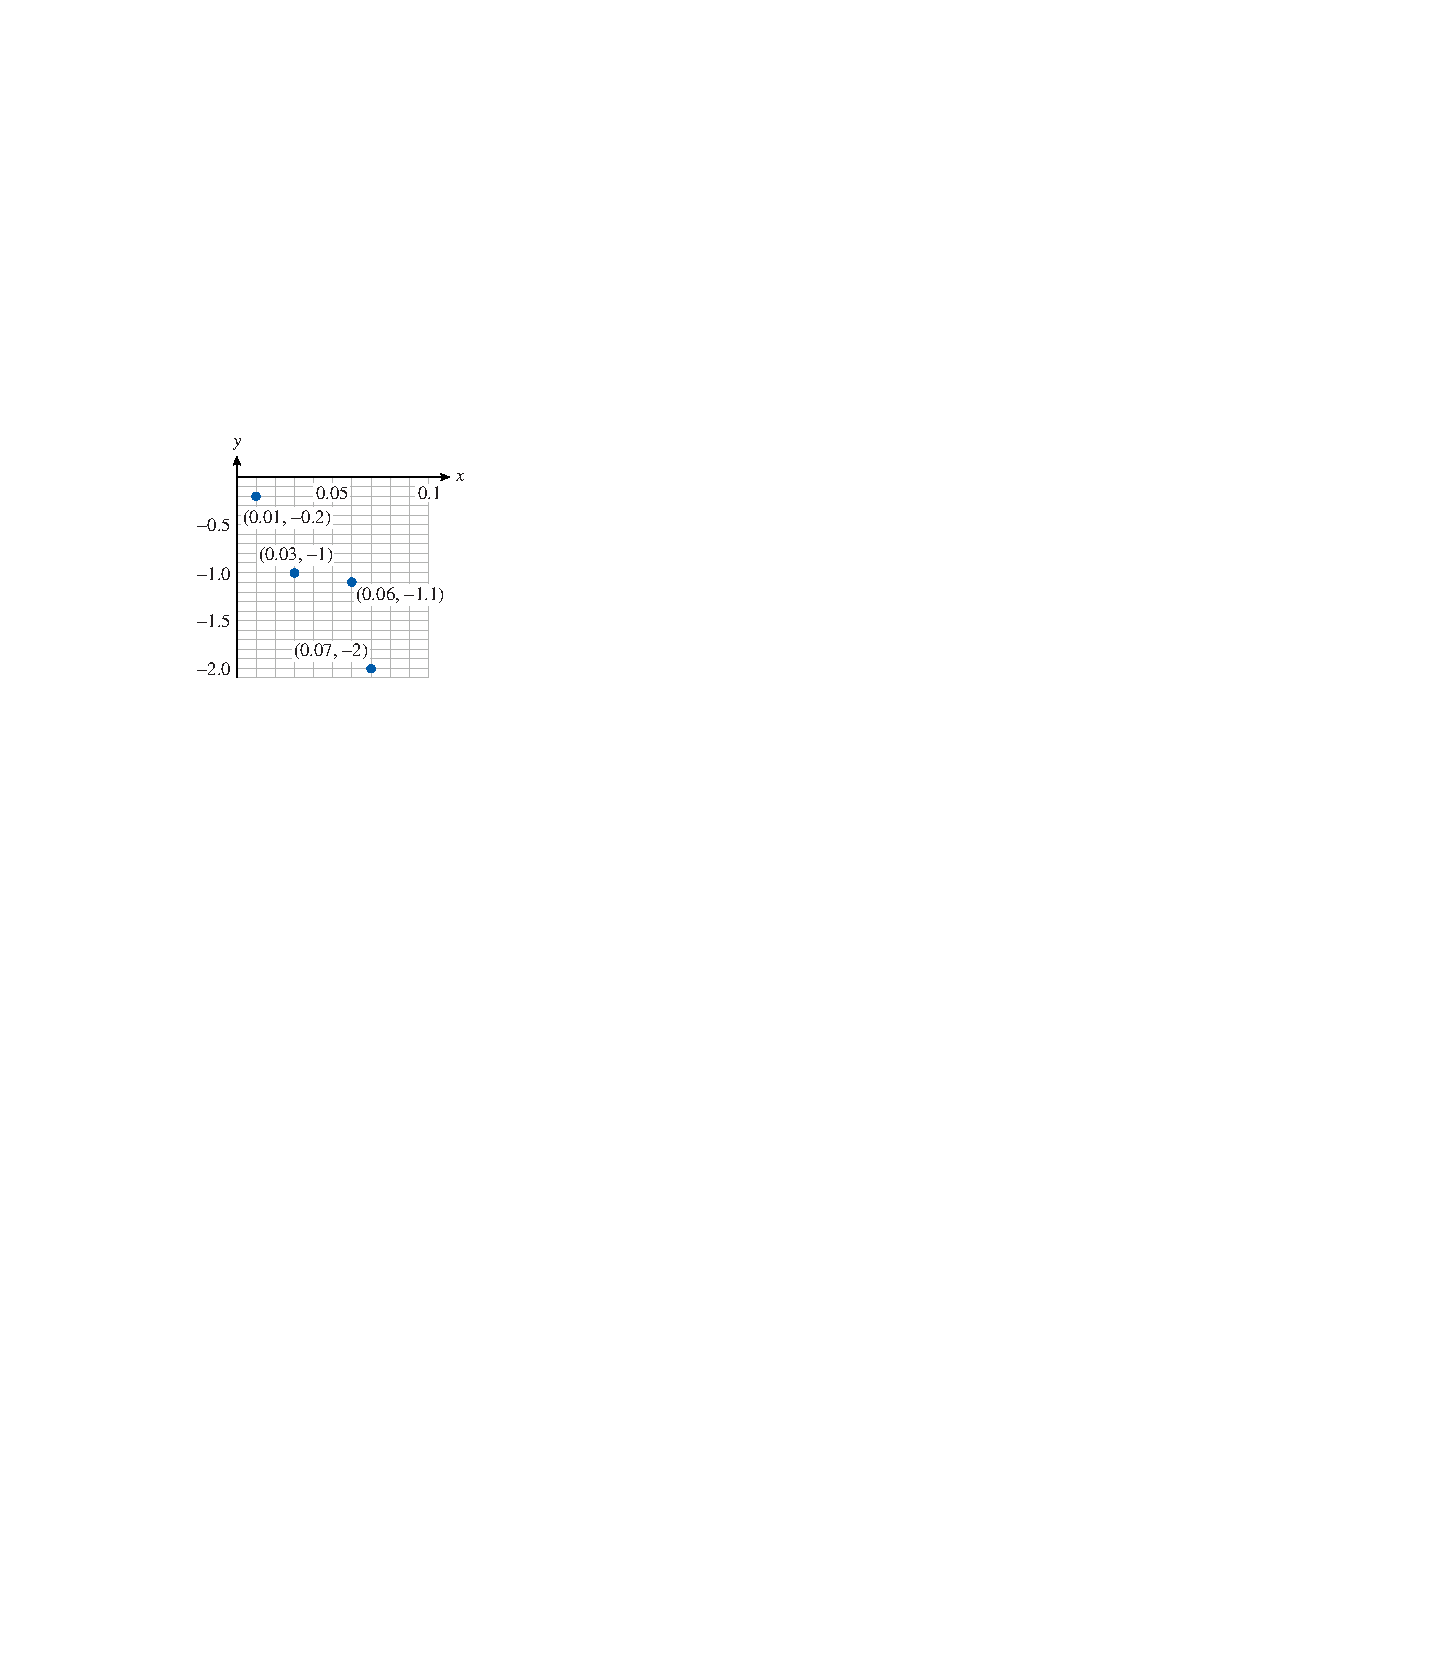
\includegraphics[width=0.5\linewidth]{images/fig-ans-1-1-11}
%
\exercise[12.]\hypertarget{exercise-19}{}\begin{tabular}{AlAcAcAcAcA}\hrulethick
\(x\)&\(0.003\)&\(0.005\)&\(0.008\)&\(0.011\)\tabularnewline\hrulethin
\(y\)&\(6\)&\(2\)&\(1.5\)&\(1\)\tabularnewline\hrulethin
\end{tabular}
%
\end{exercisegroup}
\par\smallskip\noindent
\hypertarget{exercisegroup-2}{}\par\noindent For Problems 13-18, \leavevmode%
\begin{enumerate}[label=(\alph*)]
\item\hypertarget{li-163}{}Find the intercepts of the graph.%
\item\hypertarget{li-164}{}Graph the equation by the intercept method.%
\end{enumerate}
%
\begin{exercisegroup}(3)
\exercise[13.]\hypertarget{exercise-20}{}\(x + 2y = 8\)%
\par\smallskip
\noindent\textbf{Answer.}\hypertarget{answer-14}{}\quad
\leavevmode%
\begin{enumerate}[label=\alph*]
\item\hypertarget{li-165}{}\((8, 0), (0, 4)\)%
\item\hypertarget{li-166}{}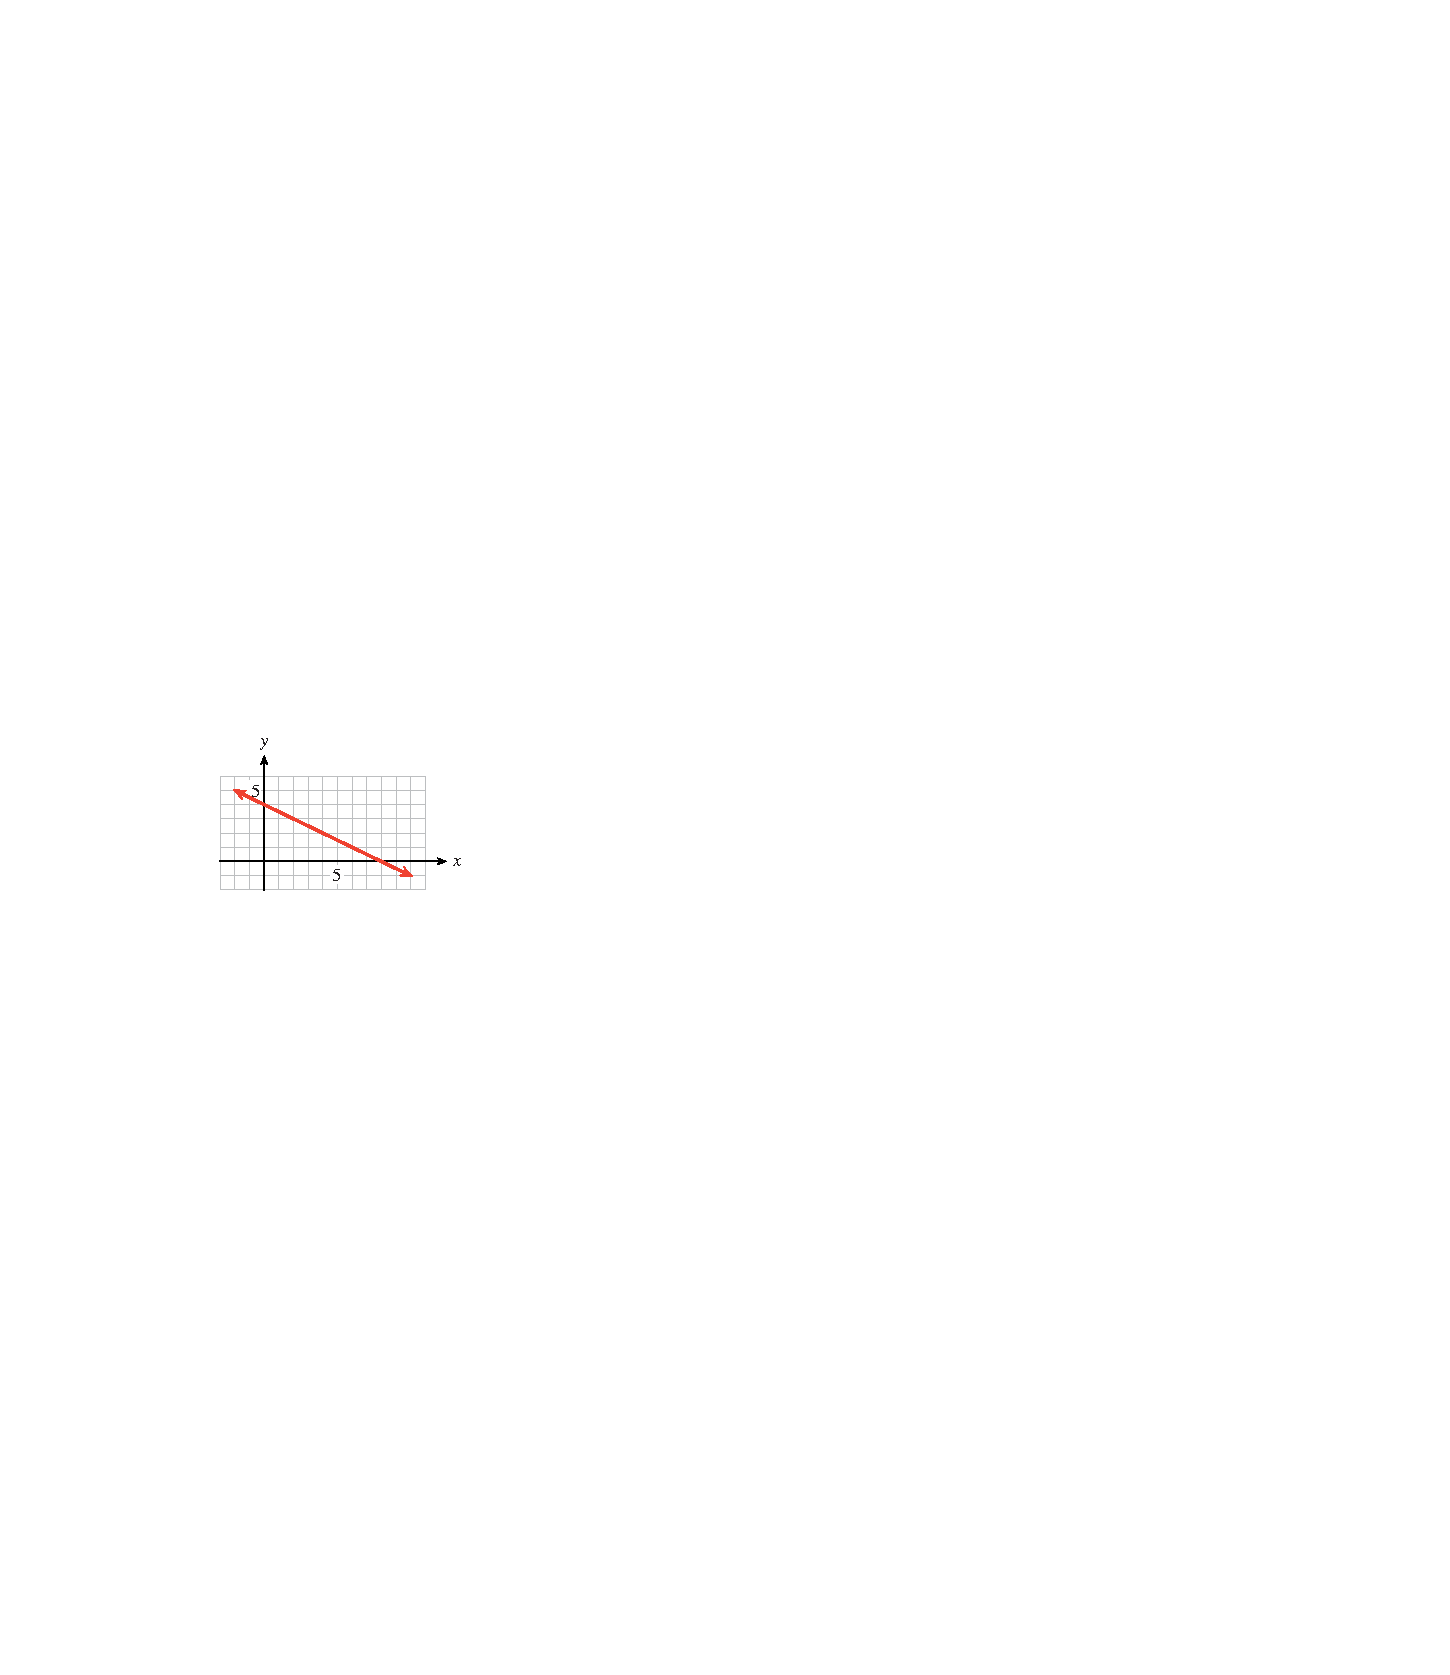
\includegraphics[width=0.5\linewidth]{images/fig-ans-1-1-13}
%
\end{enumerate}
%
\exercise[14.]\hypertarget{exercise-21}{}\(2x - y = 6\)%
\exercise[15.]\hypertarget{exercise-22}{}\(3x - 4y =12\)%
\par\smallskip
\noindent\textbf{Answer.}\hypertarget{answer-15}{}\quad
\leavevmode%
\begin{enumerate}[label=\alph*]
\item\hypertarget{li-167}{}\((4, 0), (0, -3)\)%
\item\hypertarget{li-168}{}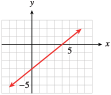
\includegraphics[width=0.5\linewidth]{images/fig-ans-1-1-15}
%
\end{enumerate}
%
\exercise[16.]\hypertarget{exercise-23}{}\(2x + 6y = 6\)%
\exercise[17.]\hypertarget{exercise-24}{}\(\displaystyle{\frac{x}{9}- \frac{y}{4}= 1}\)%
\par\smallskip
\noindent\textbf{Answer.}\hypertarget{answer-16}{}\quad
\leavevmode%
\begin{enumerate}[label=\alph*]
\item\hypertarget{li-169}{}\((9, 0), (0, -4)\)%
\item\hypertarget{li-170}{}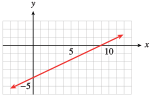
\includegraphics[width=0.5\linewidth]{images/fig-ans-1-1-17}
%
\end{enumerate}
%
\exercise[18.]\hypertarget{exercise-25}{}\(\displaystyle{\frac{x}{5}+ \frac{y}{8}= 1}\)%
\end{exercisegroup}
\par\smallskip\noindent
\hypertarget{exercisegroup-3}{}\par\noindent For Problems 19-24, \leavevmode%
\begin{enumerate}[label=(\alph*)]
\item\hypertarget{li-171}{}Find the intercepts of the graph.%
\item\hypertarget{li-172}{}Use the intercepts to choose scales for the axes, and then graph the equation by the intercept method.%
\end{enumerate}
%
\begin{exercisegroup}(2)
\exercise[19.]\hypertarget{exercise-26}{}\(20x = 30y - 45,000\)%
\par\smallskip
\noindent\textbf{Answer.}\hypertarget{answer-17}{}\quad
\leavevmode%
\begin{enumerate}[label=\alph*]
\item\hypertarget{li-173}{}\((-2250, 0), (0, 1500)\)%
\item\hypertarget{li-174}{}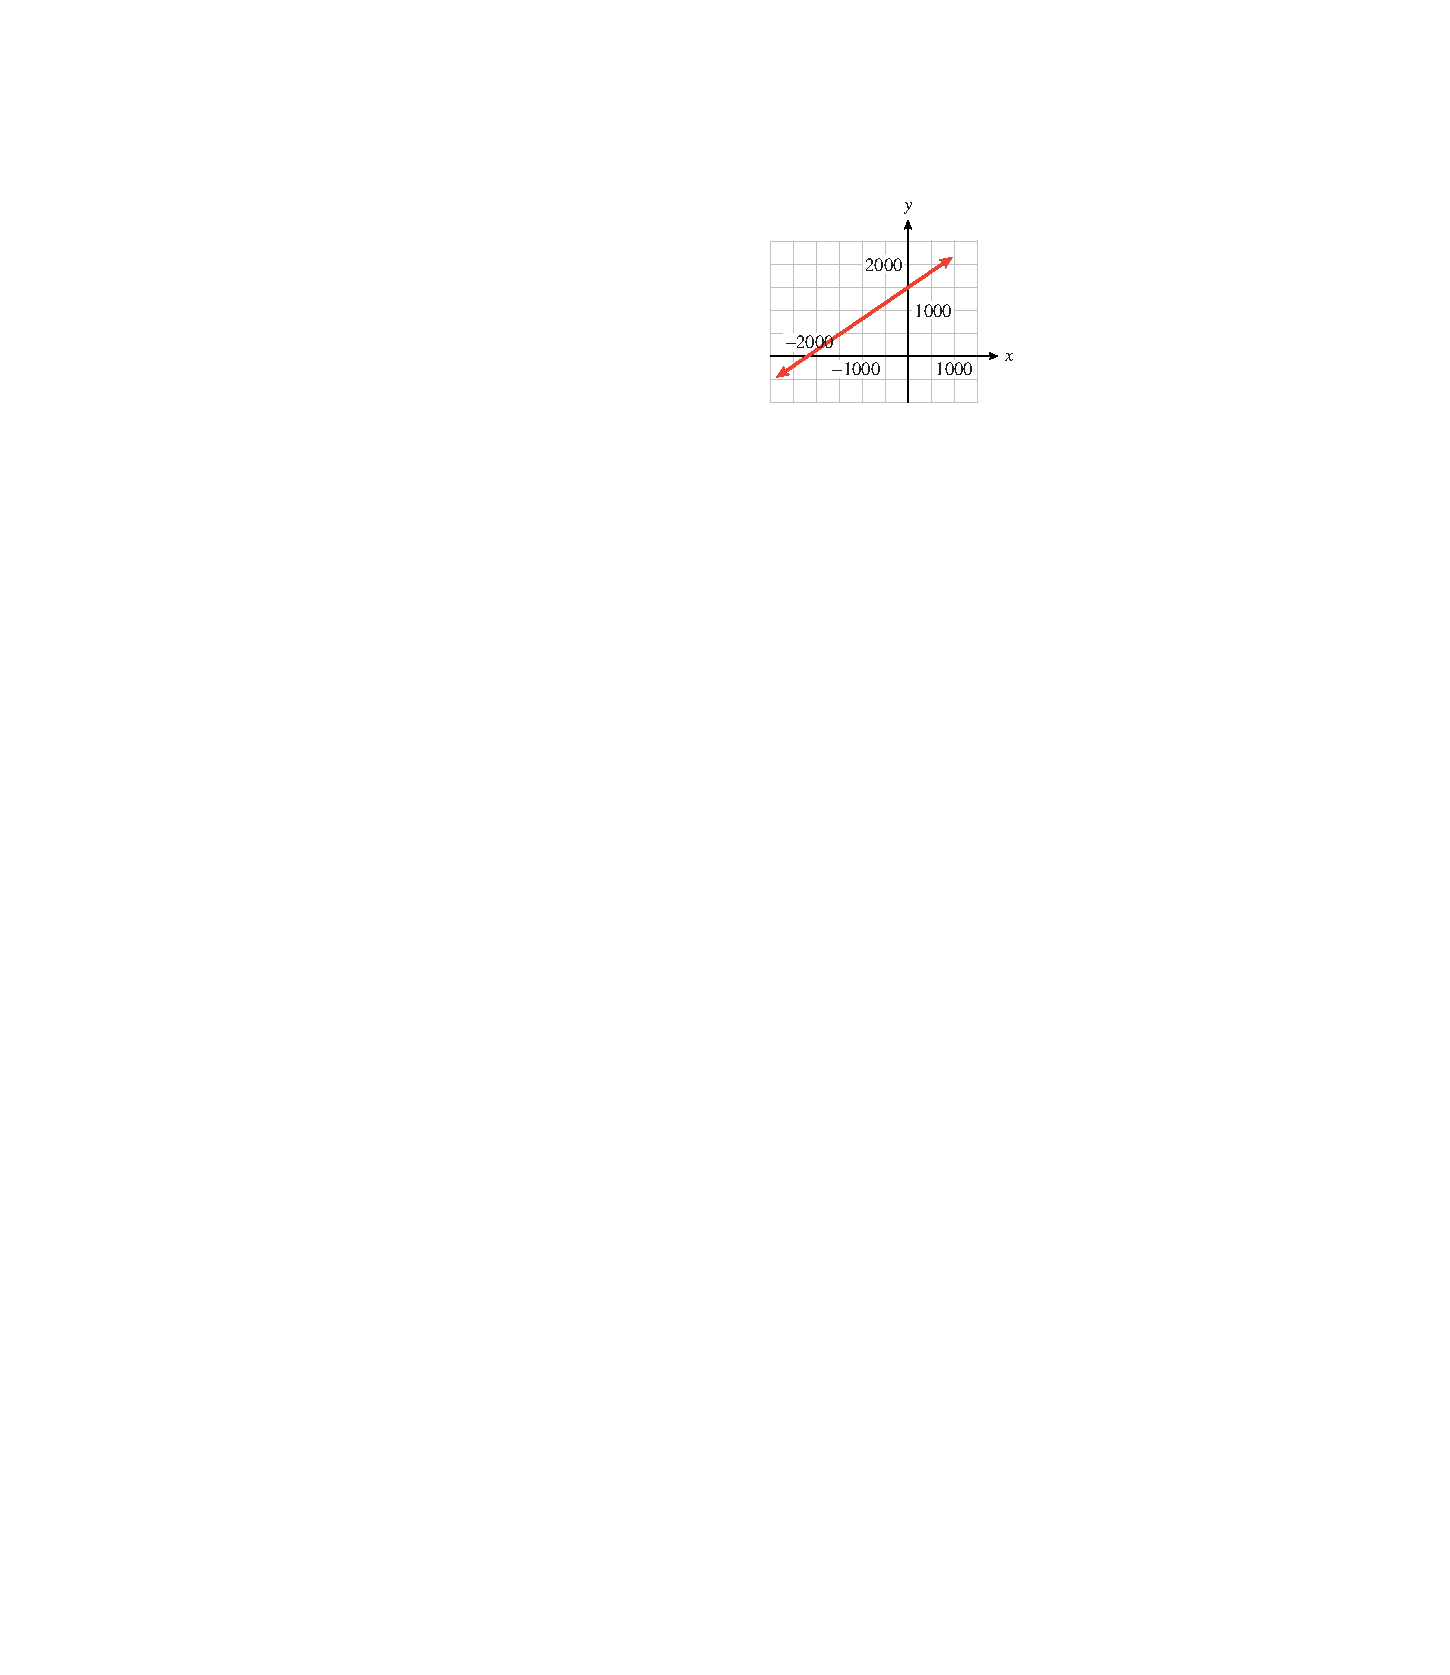
\includegraphics[width=0.5\linewidth]{images/fig-ans-1-1-19}
%
\end{enumerate}
%
\exercise[20.]\hypertarget{exercise-27}{}\(30x = 45y + 60,000\)%
\exercise[21.]\hypertarget{exercise-28}{}\(0.4x + 1.2y = 4.8\)%
\par\smallskip
\noindent\textbf{Answer.}\hypertarget{answer-18}{}\quad
\leavevmode%
\begin{enumerate}[label=\alph*]
\item\hypertarget{li-175}{}\((12, 0), (0, 4)\)%
\item\hypertarget{li-176}{}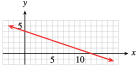
\includegraphics[width=0.5\linewidth]{images/fig-ans-1-1-21}
%
\end{enumerate}
%
\exercise[22.]\hypertarget{exercise-29}{}\(3.2x - 0.8y = 12.8\)%
\exercise[23.]\hypertarget{exercise-30}{}\(\displaystyle{\frac{2x}{3}+ \frac{3y}{11}= 1}\)%
\par\smallskip
\noindent\textbf{Answer.}\hypertarget{answer-19}{}\quad
\leavevmode%
\begin{enumerate}[label=\alph*]
\item\hypertarget{li-177}{}\(\left(\dfrac{3}{2} , 0\right), \left(0, \dfrac{11}{3} \right)\)%
\item\hypertarget{li-178}{}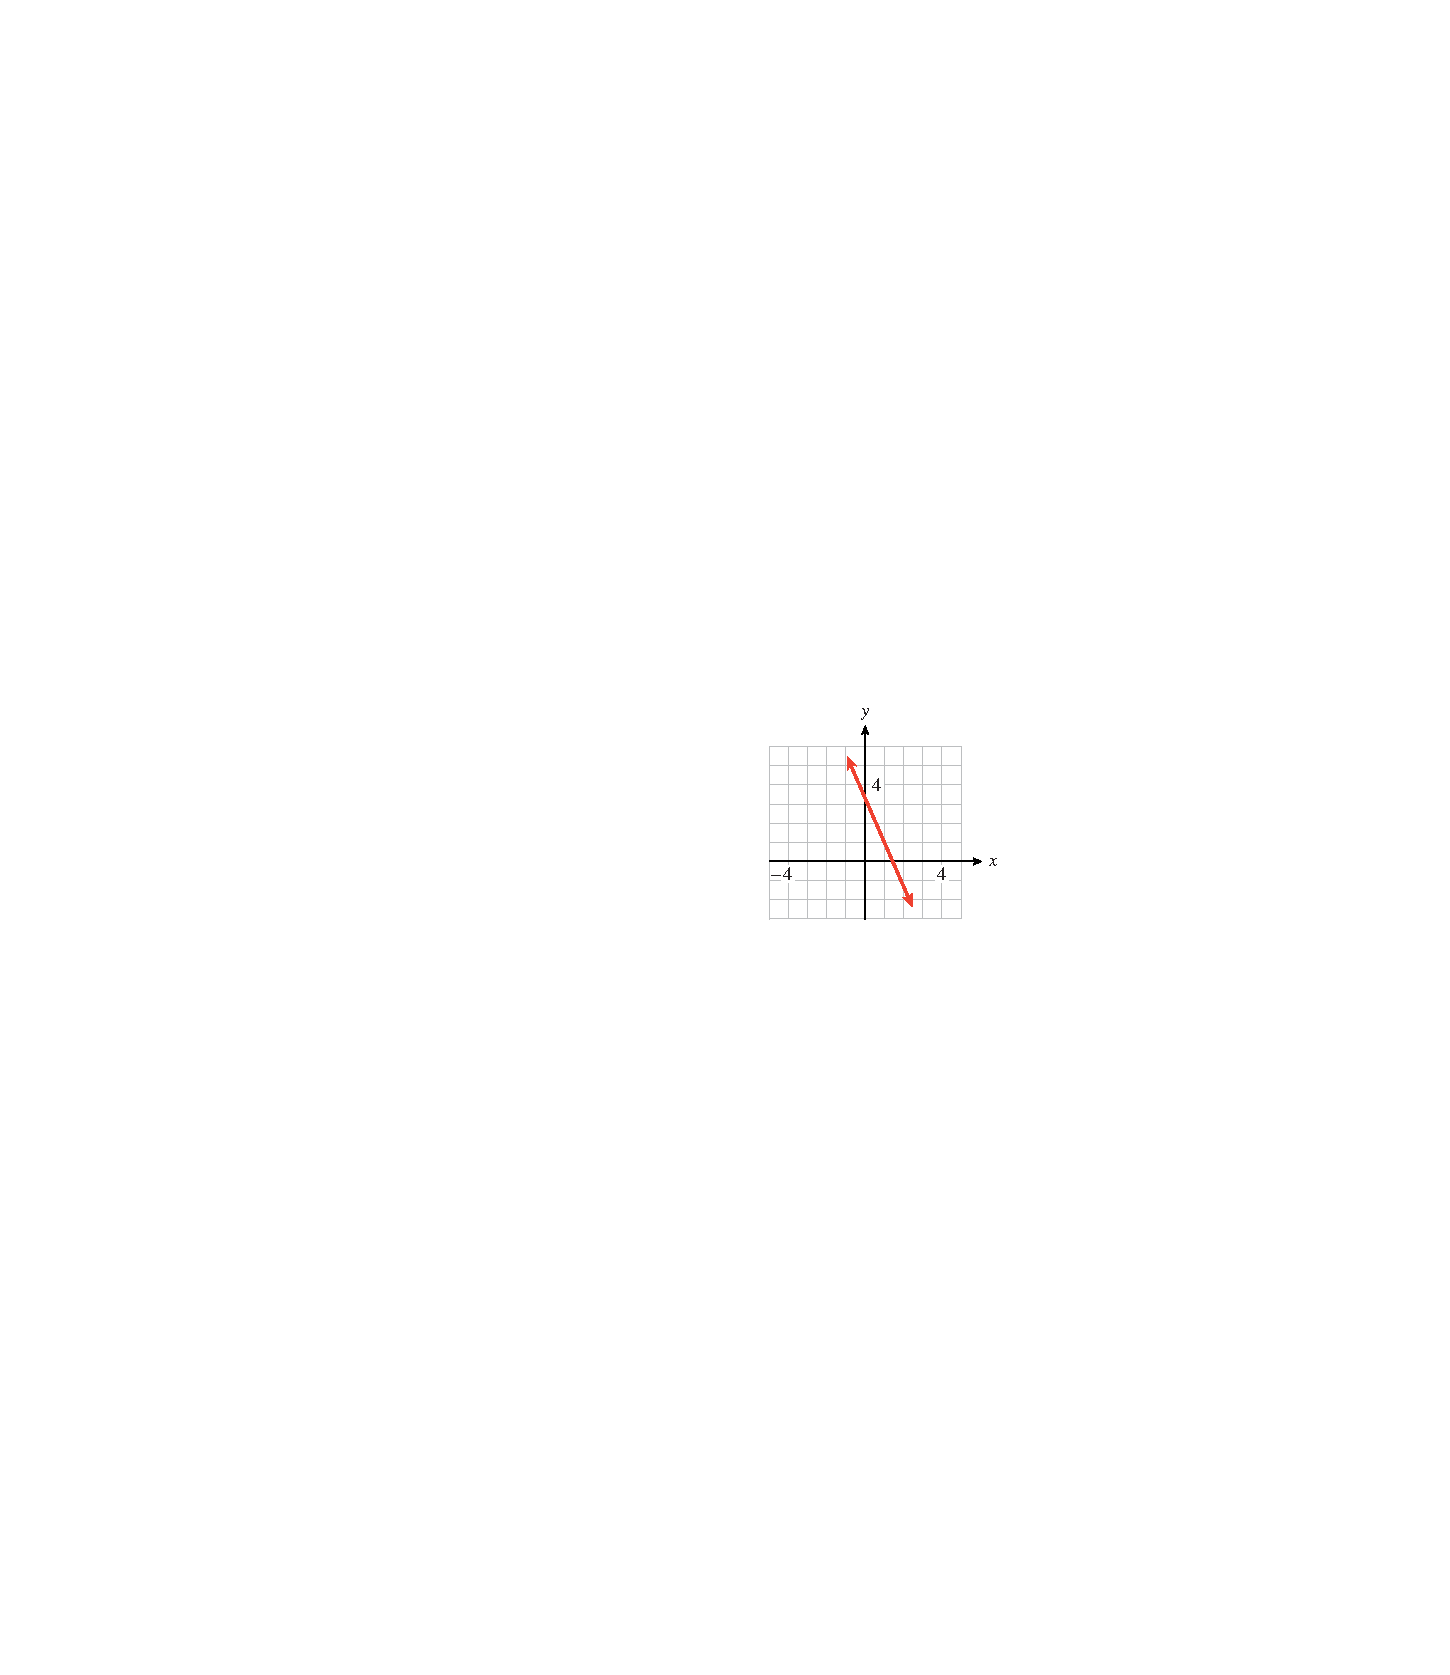
\includegraphics[width=0.5\linewidth]{images/fig-ans-1-1-23}
%
\end{enumerate}
%
\exercise[24.]\hypertarget{exercise-31}{}\(\displaystyle{\frac{8x}{7}- \frac{2y}{7}= 1}\)%
\end{exercisegroup}
\par\smallskip\noindent
\item[25.]\hypertarget{exercise-32}{}The owner of a gas station has \(\$19,200\) to spend on unleaded gas this month. Regular unleaded costs him \(\$2.40\) per gallon, and premium unleaded costs \(\$3.20\) per gallon.%
\leavevmode%
\begin{enumerate}[label=\alph*]
\item\hypertarget{li-179}{}How much do \(x\) gallons of regular cost? How much do \(y\) gallons of premium cost?%
\item\hypertarget{li-180}{}Write an equation in general form that relates the amount of regular unleaded gasoline, \(\), the owner can buy and the amount of premium unleaded, \(y\).%
\item\hypertarget{li-181}{}Find the intercepts and sketch the graph.%
\item\hypertarget{li-182}{}What do the intercepts tell us about the amount of gasoline the owner can purchase?%
\end{enumerate}
\par\smallskip
\par\smallskip
\noindent\textbf{Answer.}\hypertarget{answer-20}{}\quad
\leavevmode%
\begin{enumerate}[label=\alph*]
\item\hypertarget{li-183}{}\(\$2.40x, \$3.20y\)%
\item\hypertarget{li-184}{}\(2.40x + 3.20y = 19,200\)%
\item\hypertarget{li-185}{}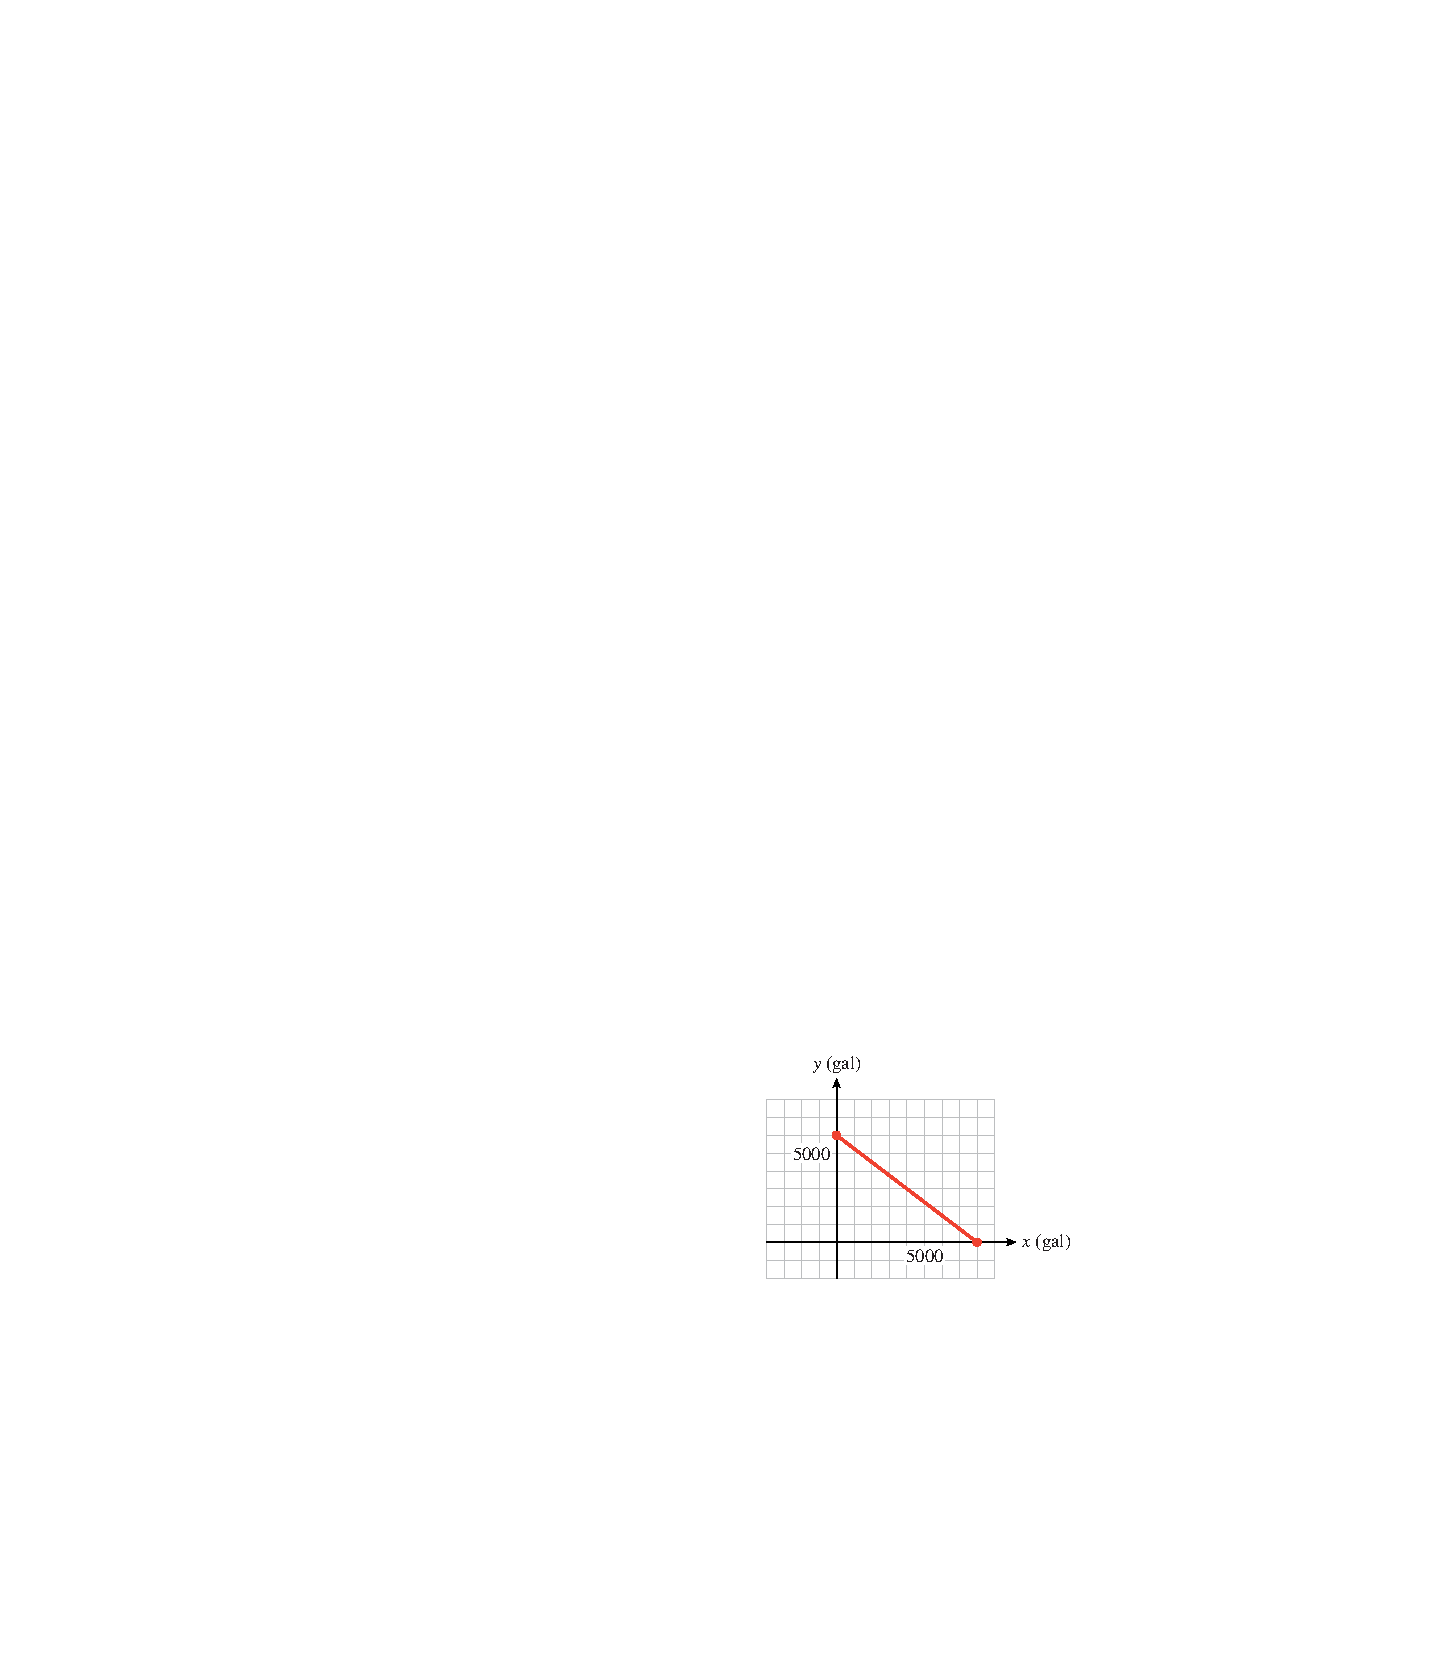
\includegraphics[width=0.5\linewidth]{images/fig-ans-1-1-25}
%
\item\hypertarget{li-186}{}The \(y\)-intercept, \(6000\) gallons, is the amount of premium that the gas station owner can buy if he buys no regular. The \(x\)-intercept, \(8000\) gallons, is the amount of regular he can buy if he buys no premium.%
\end{enumerate}
%
\item[26.]\hypertarget{exercise-33}{}Five pounds of body fat is equivalent to \(16,000\) calories. Carol can burn \(600\) calories per hour bicycling and \(400\) calories per hour swimming.%
\leavevmode%
\begin{enumerate}[label=\alph*]
\item\hypertarget{li-187}{}How many calories will Carol burn in \(\) hours of cycling? How many calories will she burn in \(y\) hours of swimming?%
\item\hypertarget{li-188}{}Write an equation in general form that relates the number of hours, \(x\), of cycling and the number of hours, \(y\), of swimming Carol needs to perform in order to lose \(5\) pounds.%
\item\hypertarget{li-189}{}Find the intercepts and sketch the graph.%
\item\hypertarget{li-190}{}What do the intercepts tell us about Carol's exercise program?%
\end{enumerate}
\par\smallskip
\item[27.]\hypertarget{exercise-34}{}Delbert must increase his daily potassium intake by \(1800\) mg. He decides to eat a combination of figs and bananas, which are both low in sodium. There are \(9\) mg potassium per gram of fig, and \(4\) mg potassium per gram of banana.%
\leavevmode%
\begin{enumerate}[label=\alph*]
\item\hypertarget{li-191}{}How much potassium is in \(x\) grams of fig? How much potassium is in \(y\) grams of banana?%
\item\hypertarget{li-192}{}Write an equation in general form that relates the number of grams, \(x\), of fig and the number of grams, \(y\), of banana Delbert needs to get \(1800\) mg of potassium.%
\item\hypertarget{li-193}{}Find the intercepts and sketch the graph.%
\item\hypertarget{li-194}{}What do the intercepts tell us about Delbert's diet?%
\end{enumerate}
\par\smallskip
\par\smallskip
\noindent\textbf{Answer.}\hypertarget{answer-21}{}\quad
\leavevmode%
\begin{enumerate}[label=\alph*]
\item\hypertarget{li-195}{}\(9x\) mg, \(4y\) mg%
\item\hypertarget{li-196}{}\(9x + 4y = 1800\)%
\item\hypertarget{li-197}{}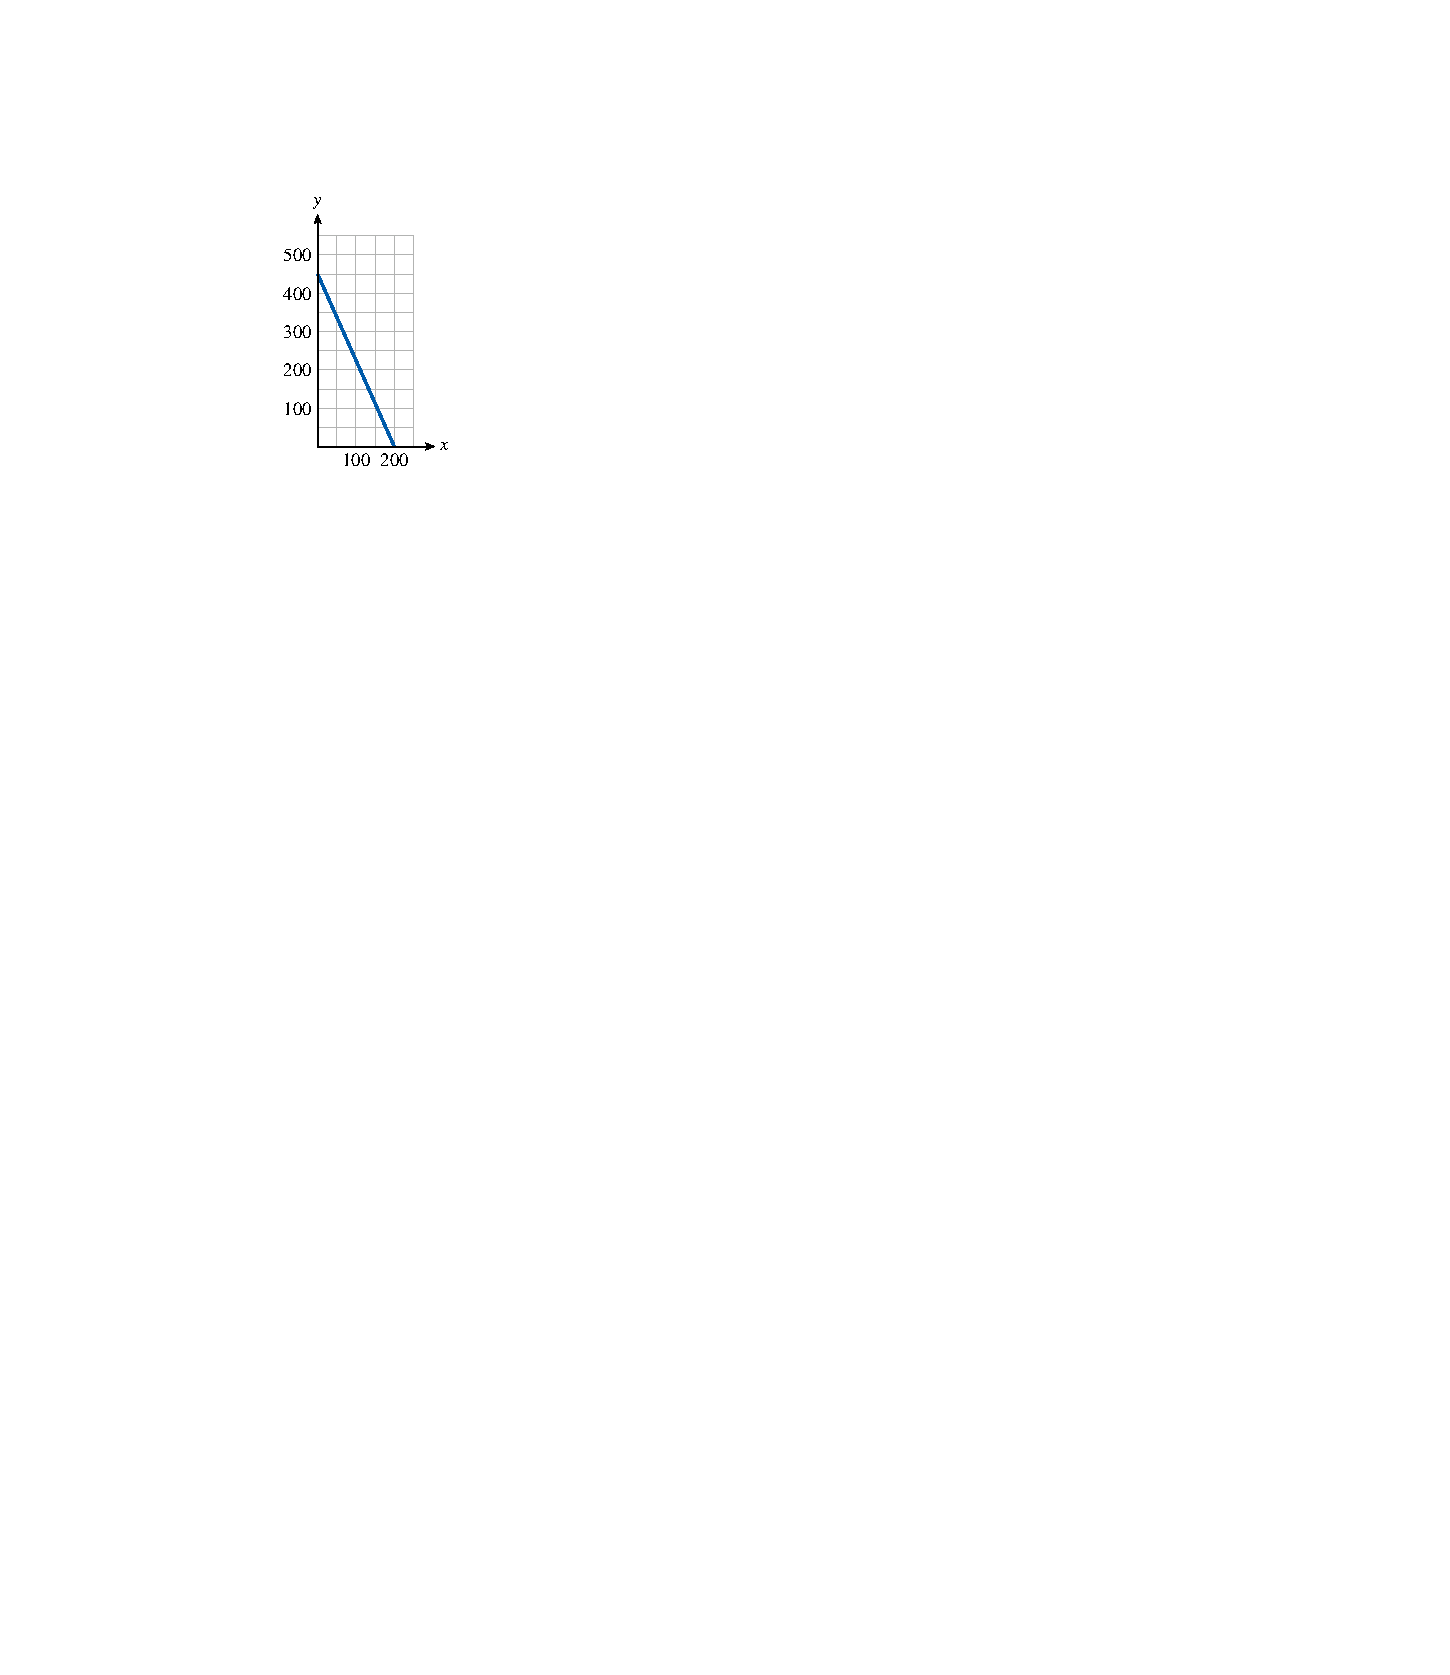
\includegraphics[width=0.35\linewidth]{images/fig-ans-1-1-27}
%
\item\hypertarget{li-198}{}The \(x\)-intercept, \(200\) grams, tells how much fig Delbert should eat if he has no bananas, and the \(y\)-intercept, \(450\) grams, tells how much banana he should eat if he has no figs.%
\end{enumerate}
%
\item[28.]\hypertarget{exercise-35}{}Leslie plans to invest some money in two CD accounts. The first account pays \(3.6\%\) interest per year, and the second account pays \(2.8\%\) interest per year. Leslie would like to earn \(\$500\) per year on her investment.%
\leavevmode%
\begin{enumerate}[label=\alph*]
\item\hypertarget{li-199}{}If Leslie invests \(x\) dollars in the first account, how much interest will she earn? How much interest will she earn if she invests \(y\) dollars in the second account?%
\item\hypertarget{li-200}{}Write an equation in general form that relates \(x\) and \(y\) if Leslie earns \(\$500\) interest.%
\item\hypertarget{li-201}{}Find the intercepts and sketch the graph.%
\item\hypertarget{li-202}{}What do the intercepts tell us about Leslie's investments?%
\end{enumerate}
\par\smallskip
\item[29.]\hypertarget{exercise-36}{}Find the intercepts of the graph for each equation.%
\leavevmode%
\begin{multicols}{2}
\begin{enumerate}[label=\alph*]
\item\hypertarget{li-203}{}\(\displaystyle{\frac{x}{3}+\frac{y}{5}=1} \)%
\item\hypertarget{li-204}{}\(\displaystyle{2x - 4y = 1} \)%
\item\hypertarget{li-205}{}\(\displaystyle{\frac{2x}{5}-\frac{2y}{3}=1} \)%
\item\hypertarget{li-206}{}\(\displaystyle{\frac{x}{p}+\frac{y}{q}=1} \)%
\item\hypertarget{li-207}{}Why is the equation \(\displaystyle{\frac{x}{a}+\frac{y}{b}=1} \) called the \terminology{intercept form} for a line?%
\end{enumerate}
\end{multicols}
\par\smallskip
\par\smallskip
\noindent\textbf{Answer.}\hypertarget{answer-22}{}\quad
\leavevmode%
\begin{multicols}{2}
\begin{enumerate}[label=\alph*]
\item\hypertarget{li-208}{}\((3,0), (0,5) \)%
\item\hypertarget{li-209}{}\(\left(\dfrac{1}{2},0\right), \left(0,\dfrac{-1}{4}\right) \)%
\item\hypertarget{li-210}{}\(\left(\dfrac{5}{2},0\right), \left(0,\dfrac{-3}{2}\right) \)%
\item\hypertarget{li-211}{}\((p,0), (0,q) \)%
\item\hypertarget{li-212}{}The value of \(a\) is the \(x\)-intercept, and the value of \(b\) is the \(y\)-intercept.%
\end{enumerate}
\end{multicols}
%
\item[30.]\hypertarget{exercise-37}{}Write an equation in intercept form (see Problem 29) for the line with the given intercepts. Then write the equation in general form.%
\leavevmode%
\begin{multicols}{2}
\begin{enumerate}[label=\alph*]
\item\hypertarget{li-213}{}\((6, 0), (0, 2) \)%
\item\hypertarget{li-214}{}\((-3, 0), (0, 8) \)%
\item\hypertarget{li-215}{}\(\left(\dfrac{3}{4}, 0\right), \left(0, \dfrac{-1}{4}\right) \)%
\item\hypertarget{li-216}{}\((v, 0), (0, -w) \)%
\item\hypertarget{li-217}{}\(\left(\dfrac{1}{H}, 0\right), \left(0, \dfrac{1}{T}\right) \)%
\end{enumerate}
\end{multicols}
\par\smallskip
\item[31.]\hypertarget{exercise-38}{}\leavevmode%
\begin{enumerate}[label=\alph*]
\item\hypertarget{li-218}{}Find the \(y\)-intercept of the line \(y = mx + b\).%
\item\hypertarget{li-219}{}Find the \(x\)-intercept of the line \(y = mx + b\).%
\end{enumerate}
%
\par\smallskip
\par\smallskip
\noindent\textbf{Answer.}\hypertarget{answer-23}{}\quad
\leavevmode%
\begin{enumerate}[label=\alph*]
\item\hypertarget{li-220}{}\((0, b)\)%
\item\hypertarget{li-221}{}\(\left(\dfrac{-b}{m},0\right)\), if \(m\ne 0\)%
\end{enumerate}
%
\item[32.]\hypertarget{exercise-39}{}\leavevmode%
\begin{enumerate}[label=\alph*]
\item\hypertarget{li-222}{}Find the \(y\)-intercept of the line \(Ax + By = C\).%
\item\hypertarget{li-223}{}Find the \(x\)-intercept of the line \(Ax + By = C\).%
\end{enumerate}
%
\par\smallskip
\end{exerciselist}
\hypertarget{exercisegroup-4}{}\par\noindent Write an equation in general form for each line.%
\begin{exercisegroup}(2)
\exercise[33.]\hypertarget{exercise-40}{}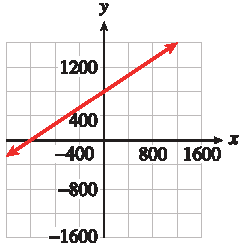
\includegraphics[width=0.8\linewidth]{images/fig-ex-1-1-33}
%
\par\smallskip
\noindent\textbf{Answer.}\hypertarget{answer-24}{}\quad
\(-2x + 3y = 2400\)%
\exercise[34.]\hypertarget{exercise-41}{}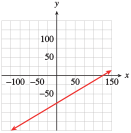
\includegraphics[width=0.8\linewidth]{images/fig-ex-1-1-34}
%
\exercise[35.]\hypertarget{exercise-42}{}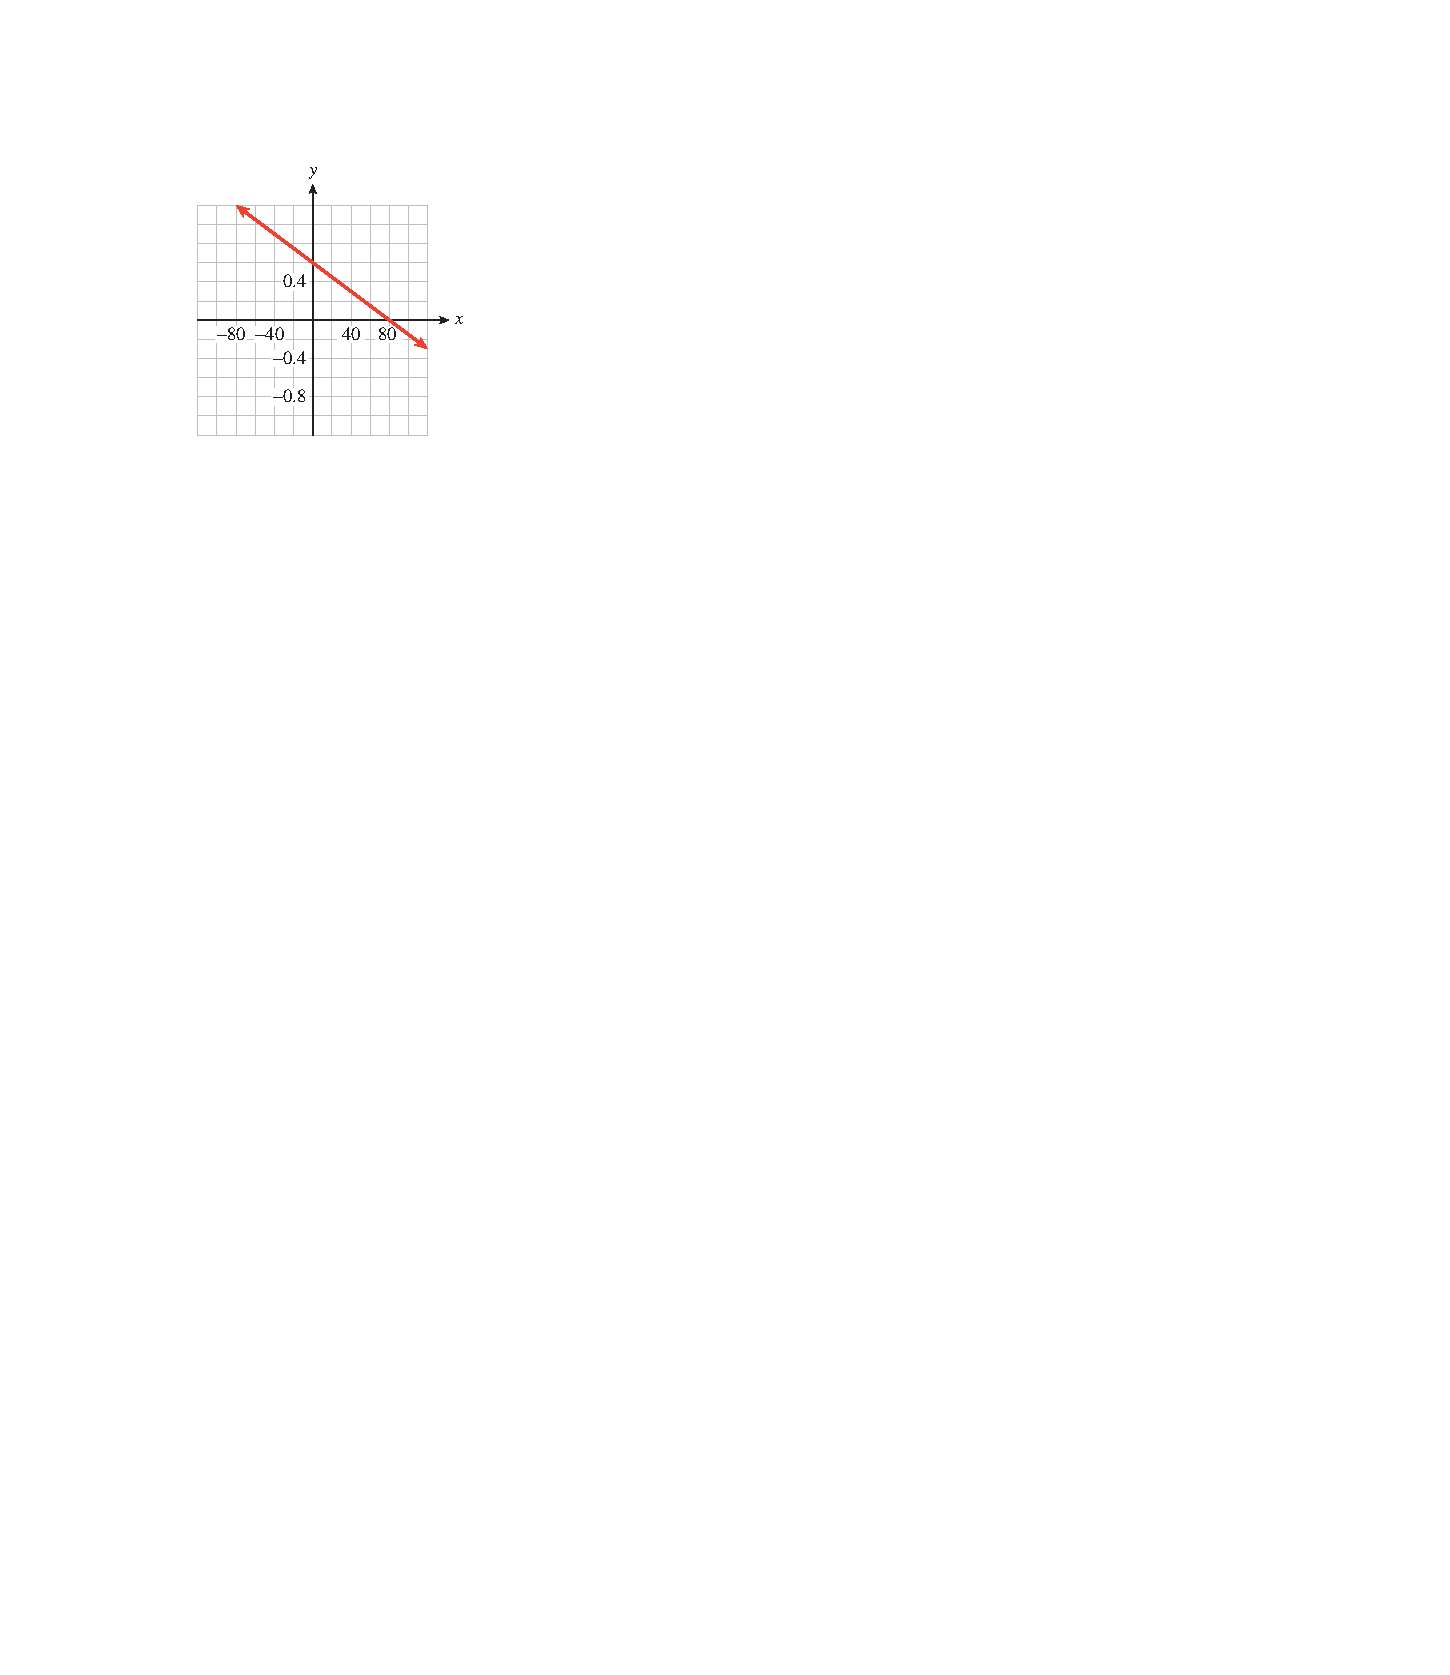
\includegraphics[width=0.8\linewidth]{images/fig-ex-1-1-35}
%
\par\smallskip
\noindent\textbf{Answer.}\hypertarget{answer-25}{}\quad
\(3x + 400y = 240\)%
\exercise[36.]\hypertarget{exercise-43}{}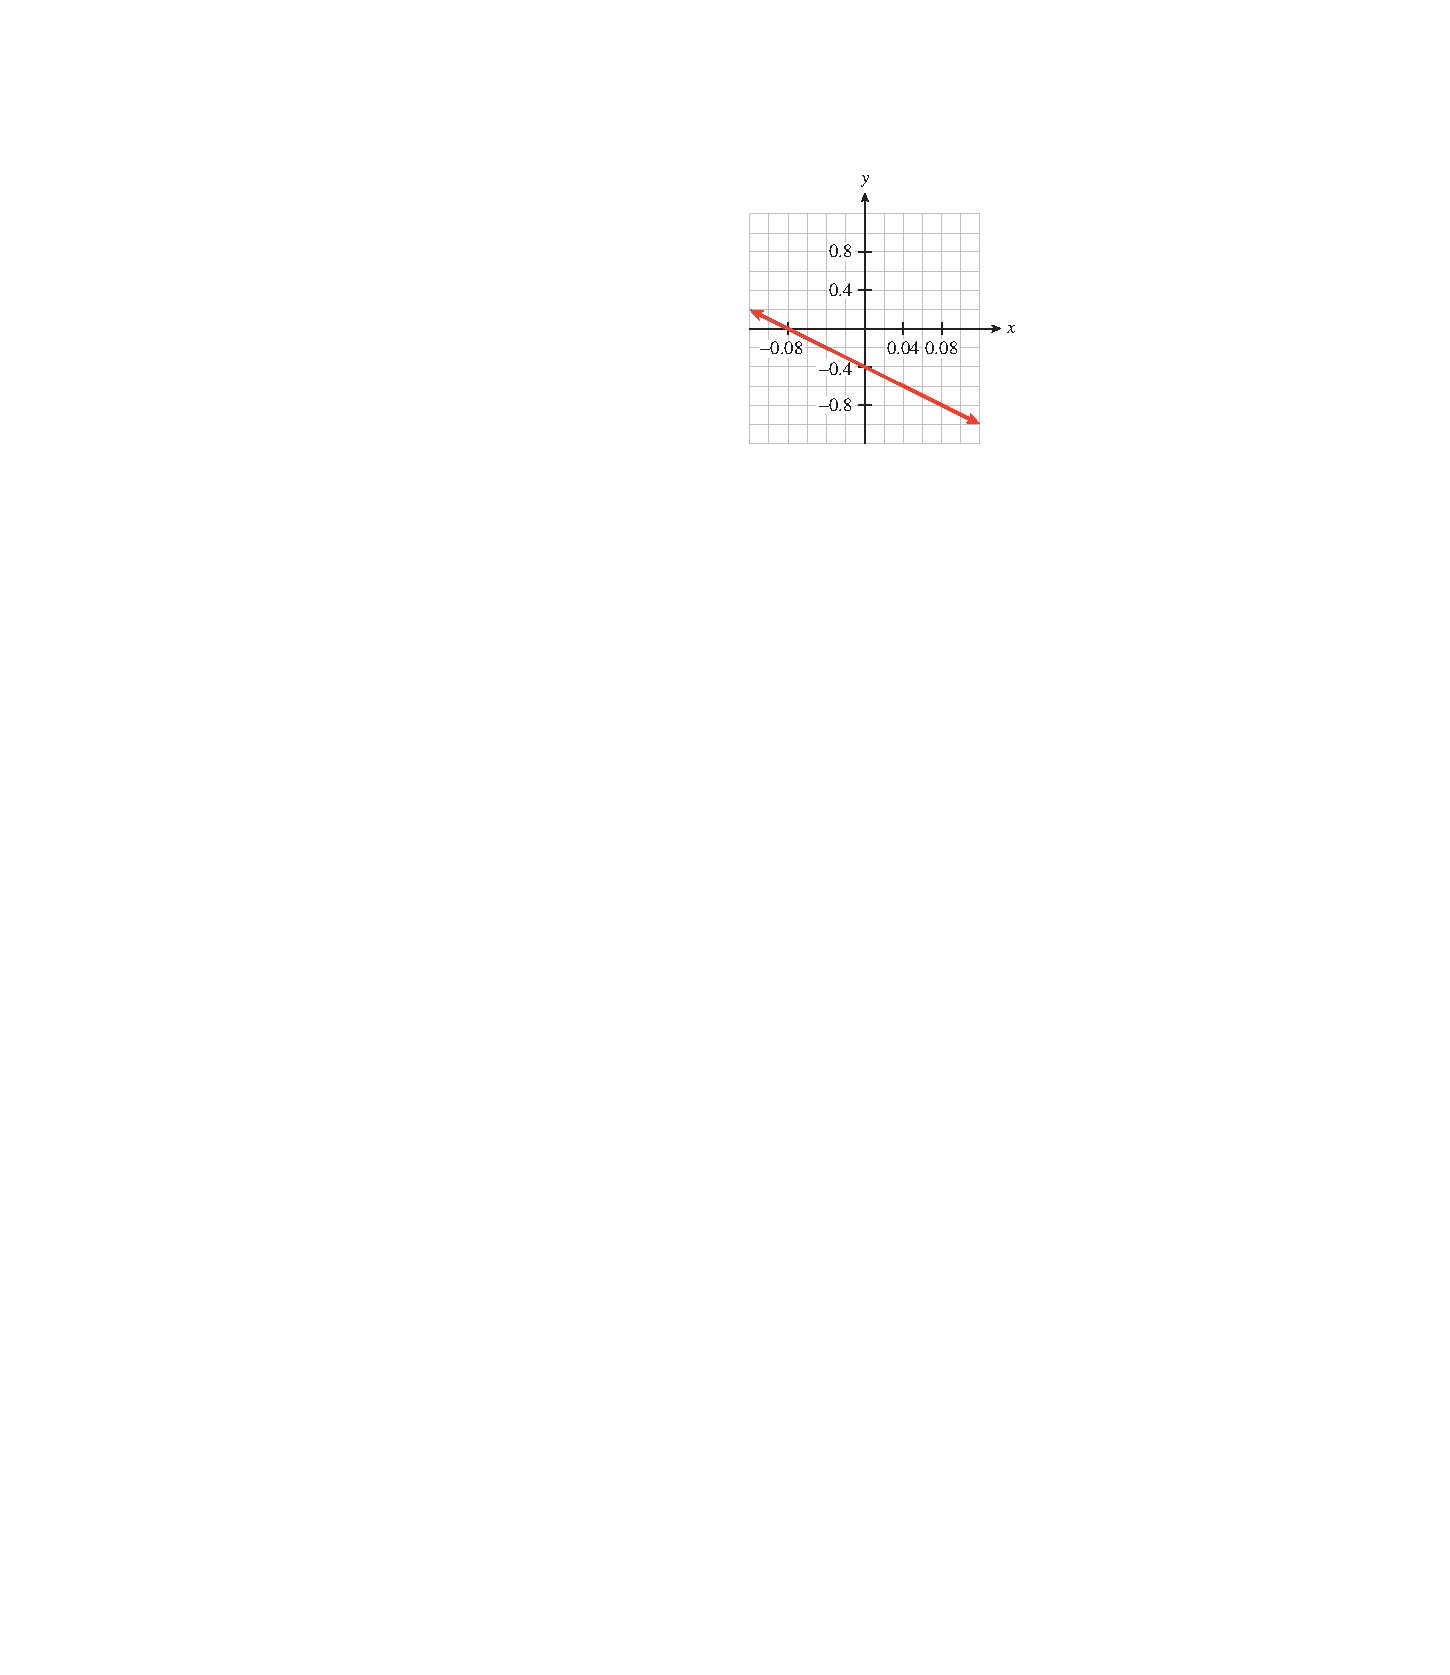
\includegraphics[width=0.8\linewidth]{images/fig-ex-1-1-36}
%
\end{exercisegroup}
\par\smallskip\noindent
\hypertarget{exercisegroup-5}{}\par\noindent For Problems 37–44, \leavevmode%
\begin{enumerate}[label=\alph*]
\item\hypertarget{li-224}{}Solve each equation for \(y\) in terms of \(x\). (See the Algebra Skills Refresher {$\langle\langle$Unresolved xref, reference "appendix-Linear-Equations-and-Inequalities"; check spelling or use "provisional" attribute$\rangle\rangle$} to review this skill.)%
\item\hypertarget{li-225}{}Graph the equation on your calculator in the specified window. (See {$\langle\langle$Unresolved xref, reference "appendix-b"; check spelling or use "provisional" attribute$\rangle\rangle$} for help with the graphing calculator.)%
\item\hypertarget{li-226}{}Make a pencil and paper sketch of the graph. Label the scales on your axes, and the coordinates of the intercepts.%
\end{enumerate}
%
\begin{exercisegroup}(2)
\exercise[37.]\hypertarget{exercise-44}{}\(2+y=6\)%
\begin{align*}
\small{\text{Xmin}} \amp = -10 \amp\amp \small{\text{Ymin}} = -10
\\
\small{\text{Xmax}} \amp = 10 \amp\amp \small{\text{Ymax}} = 10
\\
\small{\text{Xscl}} \amp = 1 \amp\amp \small{\text{Yscl}} = 1
\end{align*}
%
\par\smallskip
\noindent\textbf{Answer.}\hypertarget{answer-26}{}\quad
\leavevmode%
\begin{description}
\item[{a.}]\hypertarget{li-227}{}\(y = 6 - 2x\)%
\item[{c.}]\hypertarget{li-228}{}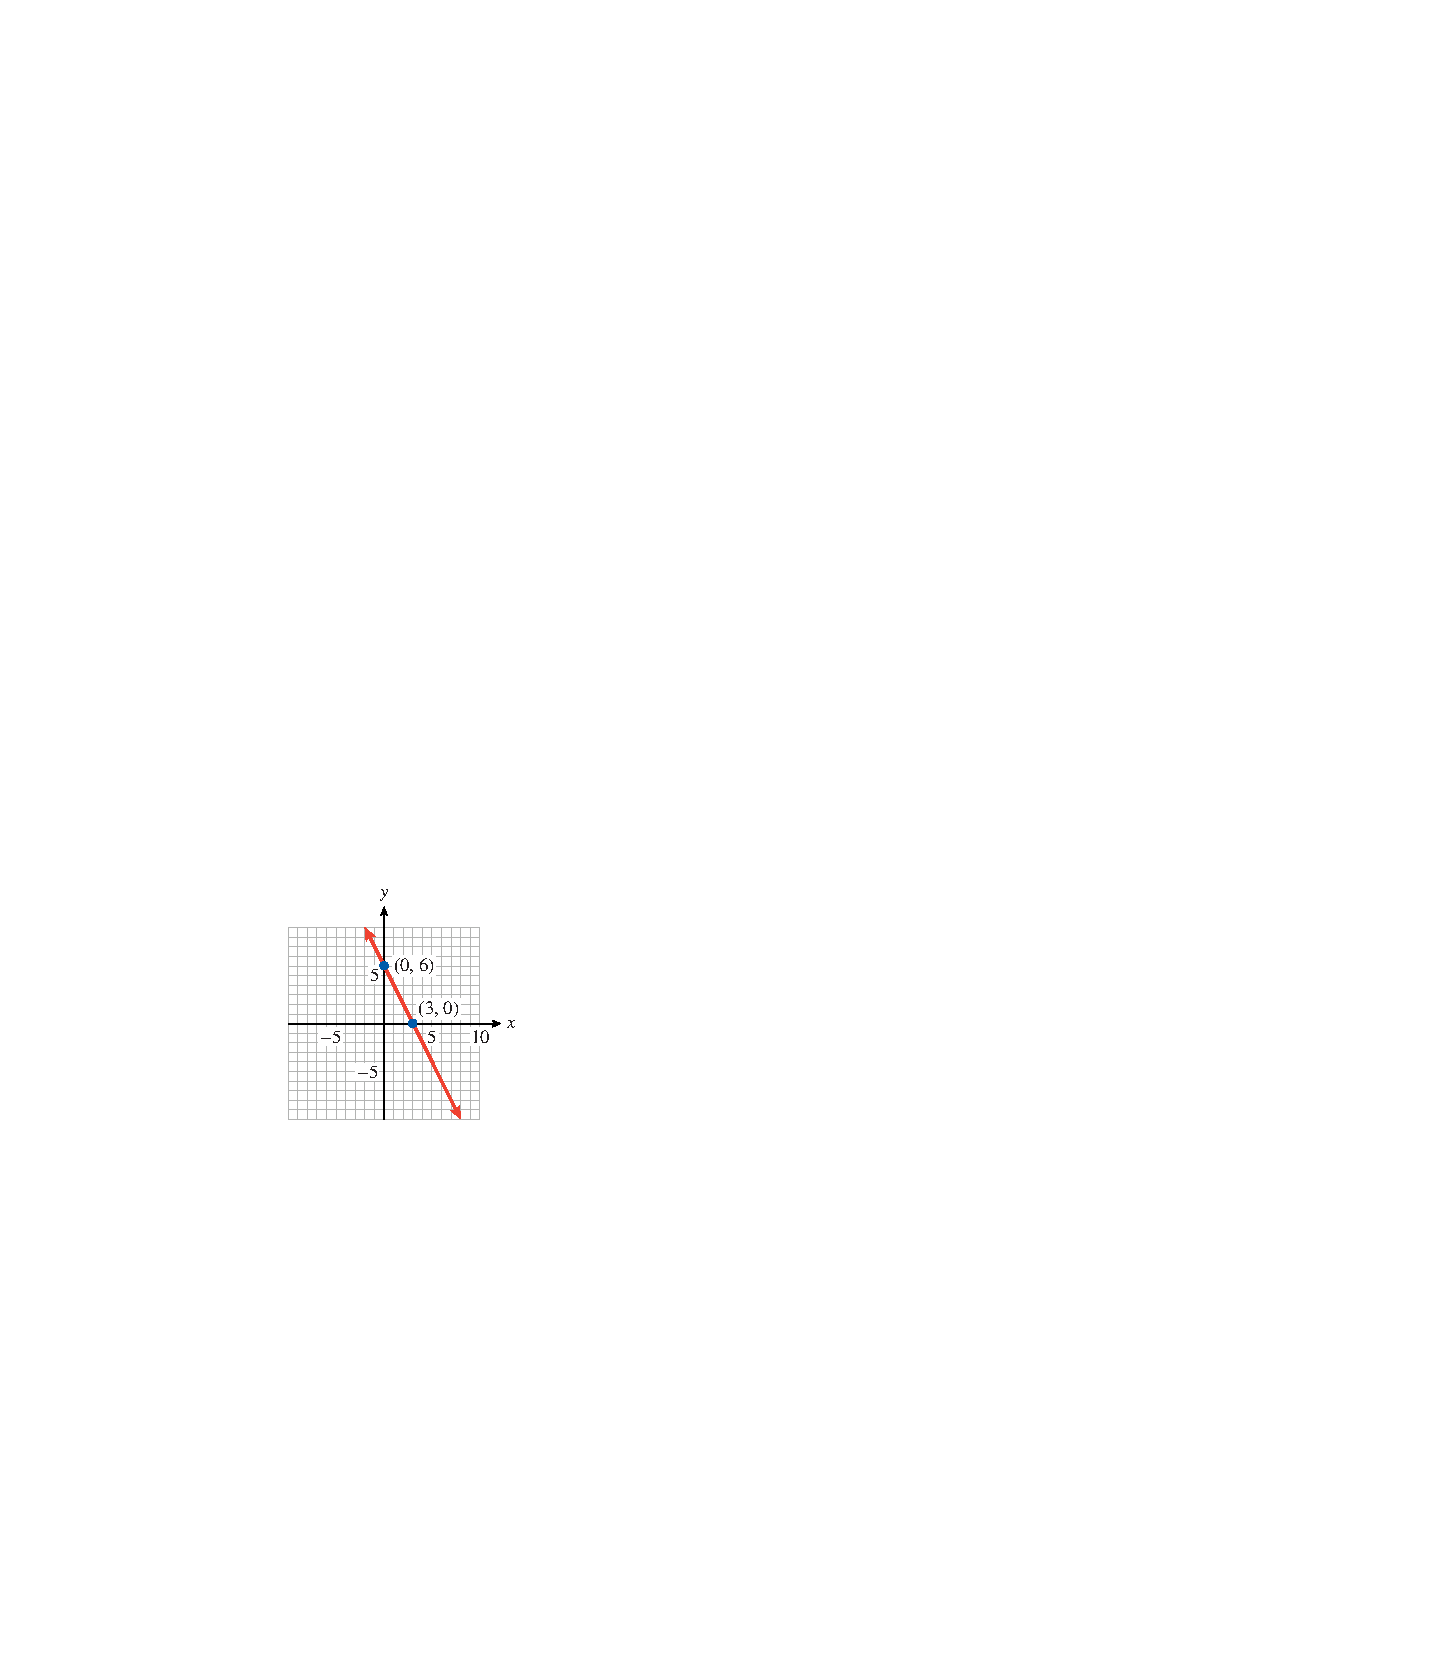
\includegraphics[width=0.5\linewidth]{images/fig-ans-1-1-37}
%
\end{description}
%
\exercise[38.]\hypertarget{exercise-45}{}\(8 - y + 3x = 0\)%
\begin{align*}
\small{\text{Xmin}} \amp = -10 \amp\amp \small{\text{Ymin}} = -10
\\
\small{\text{Xmax}} \amp = 10 \amp\amp \small{\text{Ymax}} = 10
\\
\small{\text{Xscl}} \amp = 1 \amp\amp \small{\text{Yscl}} = 1
\end{align*}
%
\exercise[39.]\hypertarget{exercise-46}{}\(3x - 4y = 1200\)%
\begin{align*}
\small{\text{Xmin}} \amp = -1000 \amp\amp \small{\text{Ymin}} = -1000
\\
\small{\text{Xmax}} \amp = 1000 \amp\amp \small{\text{Ymax}} = 1000
\\
\small{\text{Xscl}} \amp = 100 \amp\amp \small{\text{Yscl}} = 100
\end{align*}
%
\par\smallskip
\noindent\textbf{Answer.}\hypertarget{answer-27}{}\quad
\leavevmode%
\begin{description}
\item[{a.}]\hypertarget{li-229}{}\(y = \dfrac{3}{4}x-300\)%
\item[{c.}]\hypertarget{li-230}{}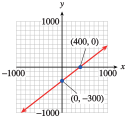
\includegraphics[width=0.5\linewidth]{images/fig-ans-1-1-39}
%
\end{description}
%
\exercise[40.]\hypertarget{exercise-47}{}\(x + 2y = 500\)%
\begin{align*}
\small{\text{Xmin}} \amp = -1000 \amp\amp \small{\text{Ymin}} = -1000
\\
\small{\text{Xmax}} \amp = 1000 \amp\amp \small{\text{Ymax}} = 1000
\\
\small{\text{Xscl}} \amp = 100 \amp\amp \small{\text{Yscl}} = 100
\end{align*}
%
\exercise[41.]\hypertarget{exercise-48}{}\(0.2x + 5y = 0.1\)%
\begin{align*}
\small{\text{Xmin}} \amp = -1 \amp\amp \small{\text{Ymin}} = -0.1
\\
\small{\text{Xmax}} \amp = 1 \amp\amp \small{\text{Ymax}} = 0.1
\\
\small{\text{Xscl}} \amp = 0.1 \amp\amp \small{\text{Yscl}} = 0.01
\end{align*}
%
\par\smallskip
\noindent\textbf{Answer.}\hypertarget{answer-28}{}\quad
\leavevmode%
\begin{description}
\item[{a.}]\hypertarget{li-231}{}\(y = 0.02 - 0.04x\)%
\item[{c.}]\hypertarget{li-232}{}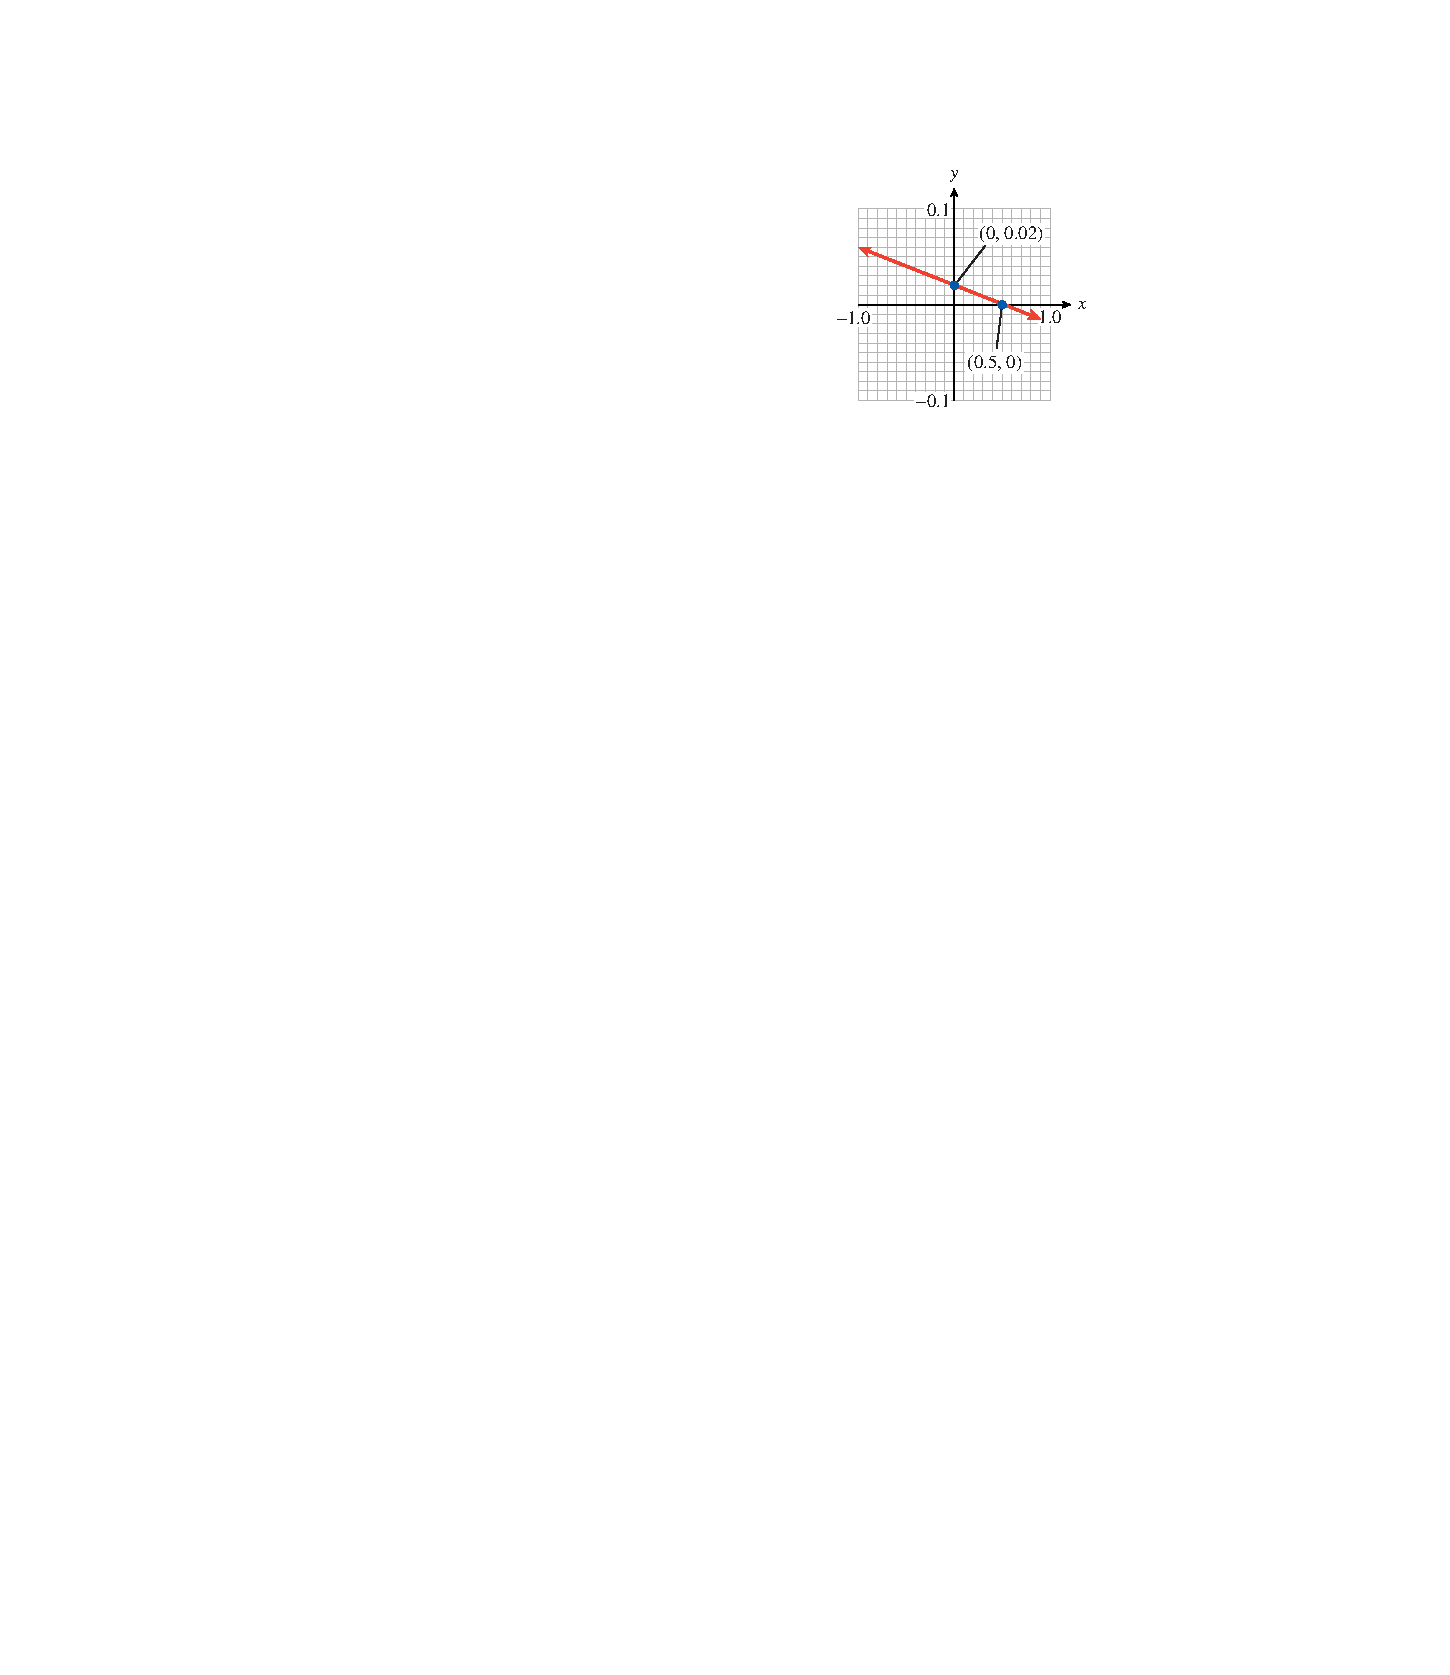
\includegraphics[width=0.5\linewidth]{images/fig-ans-1-1-41}
%
\end{description}
%
\exercise[42.]\hypertarget{exercise-49}{}\(1.2x - 4.2y = 3.6\)%
\begin{align*}
\small{\text{Xmin}} \amp = -1 \amp\amp \small{\text{Ymin}} = -1
\\
\small{\text{Xmax}} \amp = 4 \amp\amp \small{\text{Ymax}} = 1
\\
\small{\text{Xscl}} \amp = 0.2 \amp\amp \small{\text{Yscl}} = 0.1
\end{align*}
%
\exercise[43.]\hypertarget{exercise-50}{}\(70x + 3y = y + 420\)%
\begin{align*}
\small{\text{Xmin}} \amp = 0 \amp\amp \small{\text{Ymin}} = 0
\\
\small{\text{Xmax}} \amp = 10 \amp\amp \small{\text{Ymax}} = 250
\\
\small{\text{Xscl}} \amp = 1 \amp\amp \small{\text{Yscl}} = 25
\end{align*}
%
\par\smallskip
\noindent\textbf{Answer.}\hypertarget{answer-29}{}\quad
\leavevmode%
\begin{description}
\item[{a.}]\hypertarget{li-233}{}\(y = 210 - 35x\)%
\item[{c.}]\hypertarget{li-234}{}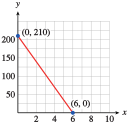
\includegraphics[width=0.5\linewidth]{images/fig-ans-1-1-43}
%
\end{description}
%
\exercise[44.]\hypertarget{exercise-51}{}\(40y - 5x = 780 - 20y\)%
\begin{align*}
\small{\text{Xmin}} \amp = -200 \amp\amp \small{\text{Ymin}} = 0
\\
\small{\text{Xmax}} \amp = 0 \amp\amp \small{\text{Ymax}} = 20
\\
\small{\text{Xscl}} \amp = 20 \amp\amp \small{\text{Yscl}} = 2
\end{align*}
%
\end{exercisegroup}
\par\smallskip\noindent
\hypertarget{exercisegroup-6}{}\par\noindent For Problems 45–52, \leavevmode%
\begin{enumerate}[label=\alph*]
\item\hypertarget{li-235}{}Find the \(\text{}\)- and \(y\)-intercepts.%
\item\hypertarget{li-236}{}Solve the equation for \(y\).%
\item\hypertarget{li-237}{}Choose a graphing window in which both intercepts are visible, and graph the equation on your calculator.%
\end{enumerate}
%
\begin{exercisegroup}(2)
\exercise[45.]\hypertarget{exercise-52}{}\(x + 4y = 100\)%
\par\smallskip
\noindent\textbf{Answer.}\hypertarget{answer-30}{}\quad
\leavevmode%
\begin{enumerate}[label=\alph*]
\item\hypertarget{li-238}{}\((100, 0), (0, 25)\)%
\item\hypertarget{li-239}{}\(y = 25 - \dfrac{1}{4}x\)%
\item\hypertarget{li-240}{}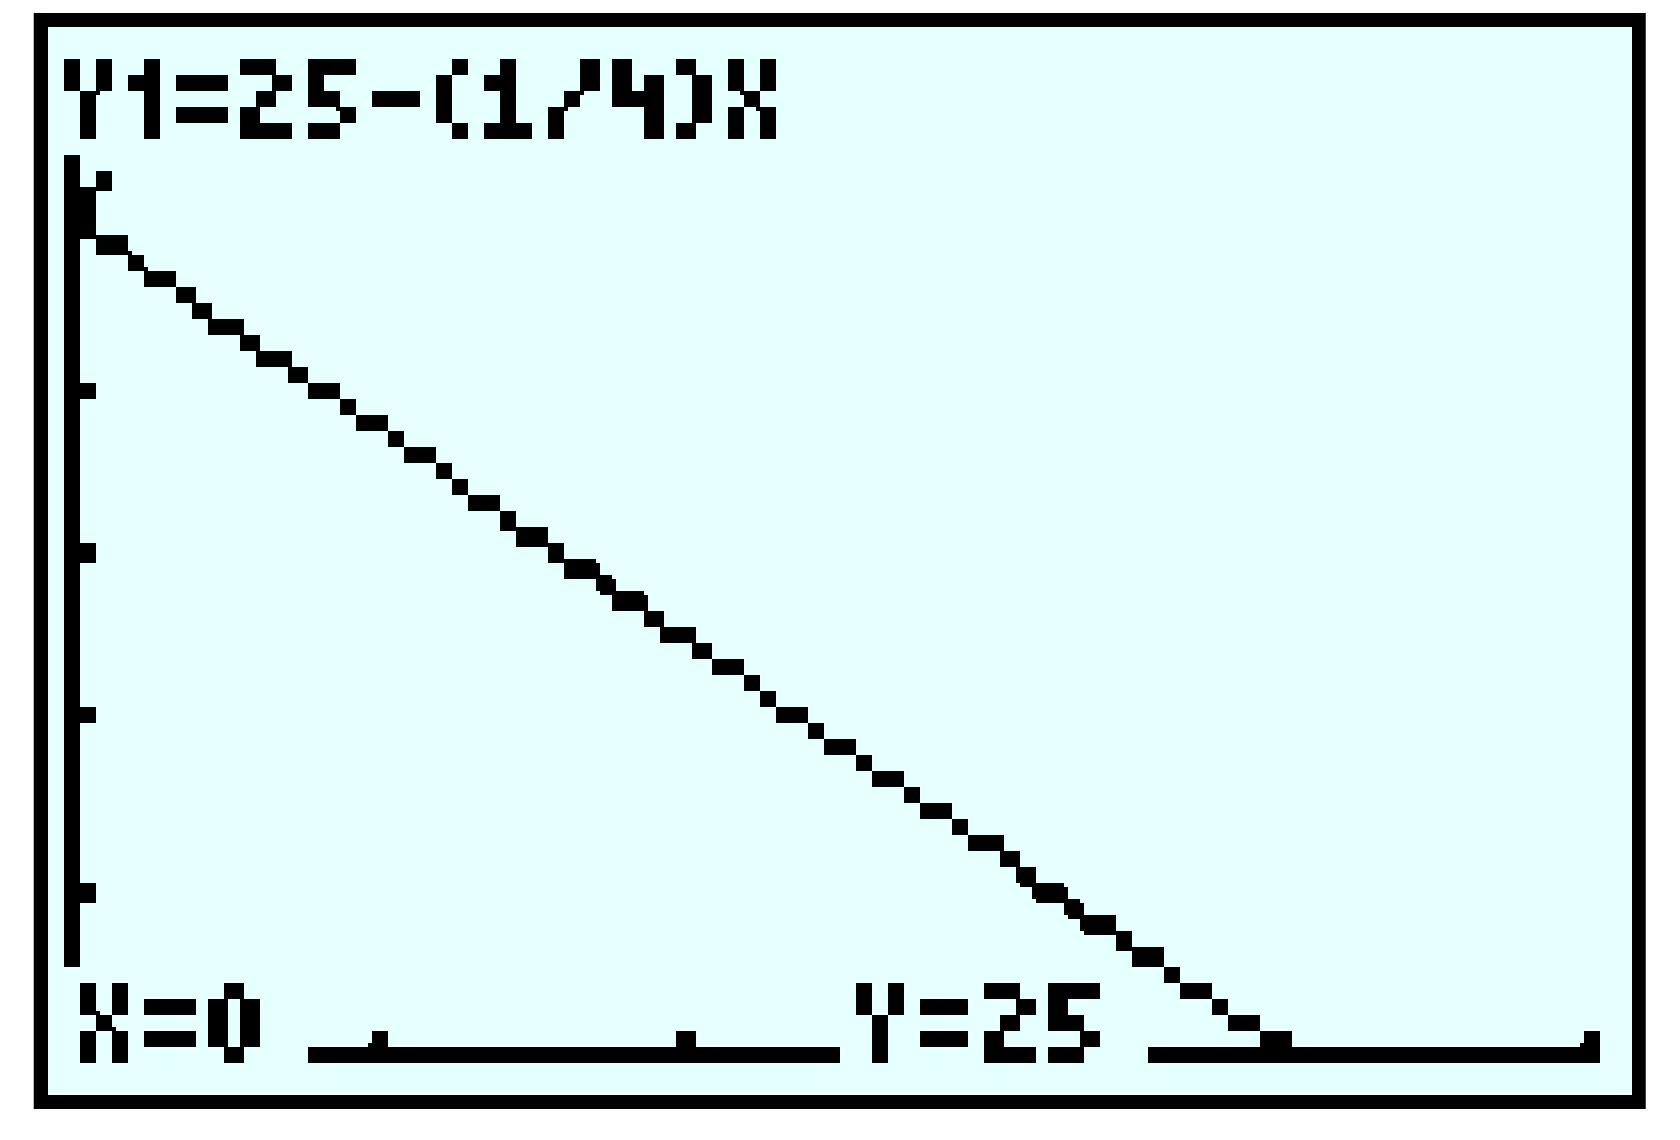
\includegraphics[width=0.5\linewidth]{images/fig-ans-1-1-45.jpg}
%
\end{enumerate}
%
\exercise[46.]\hypertarget{exercise-53}{}\(2x - 3y = -72\)%
\exercise[47.]\hypertarget{exercise-54}{}\(25x - 20y = 1\)%
\par\smallskip
\noindent\textbf{Answer.}\hypertarget{answer-31}{}\quad
\leavevmode%
\begin{enumerate}[label=\alph*]
\item\hypertarget{li-241}{}\((0.04, 0), (0, -0.05)\)%
\item\hypertarget{li-242}{}\(y = 1.25x - 0.05\)%
\item\hypertarget{li-243}{}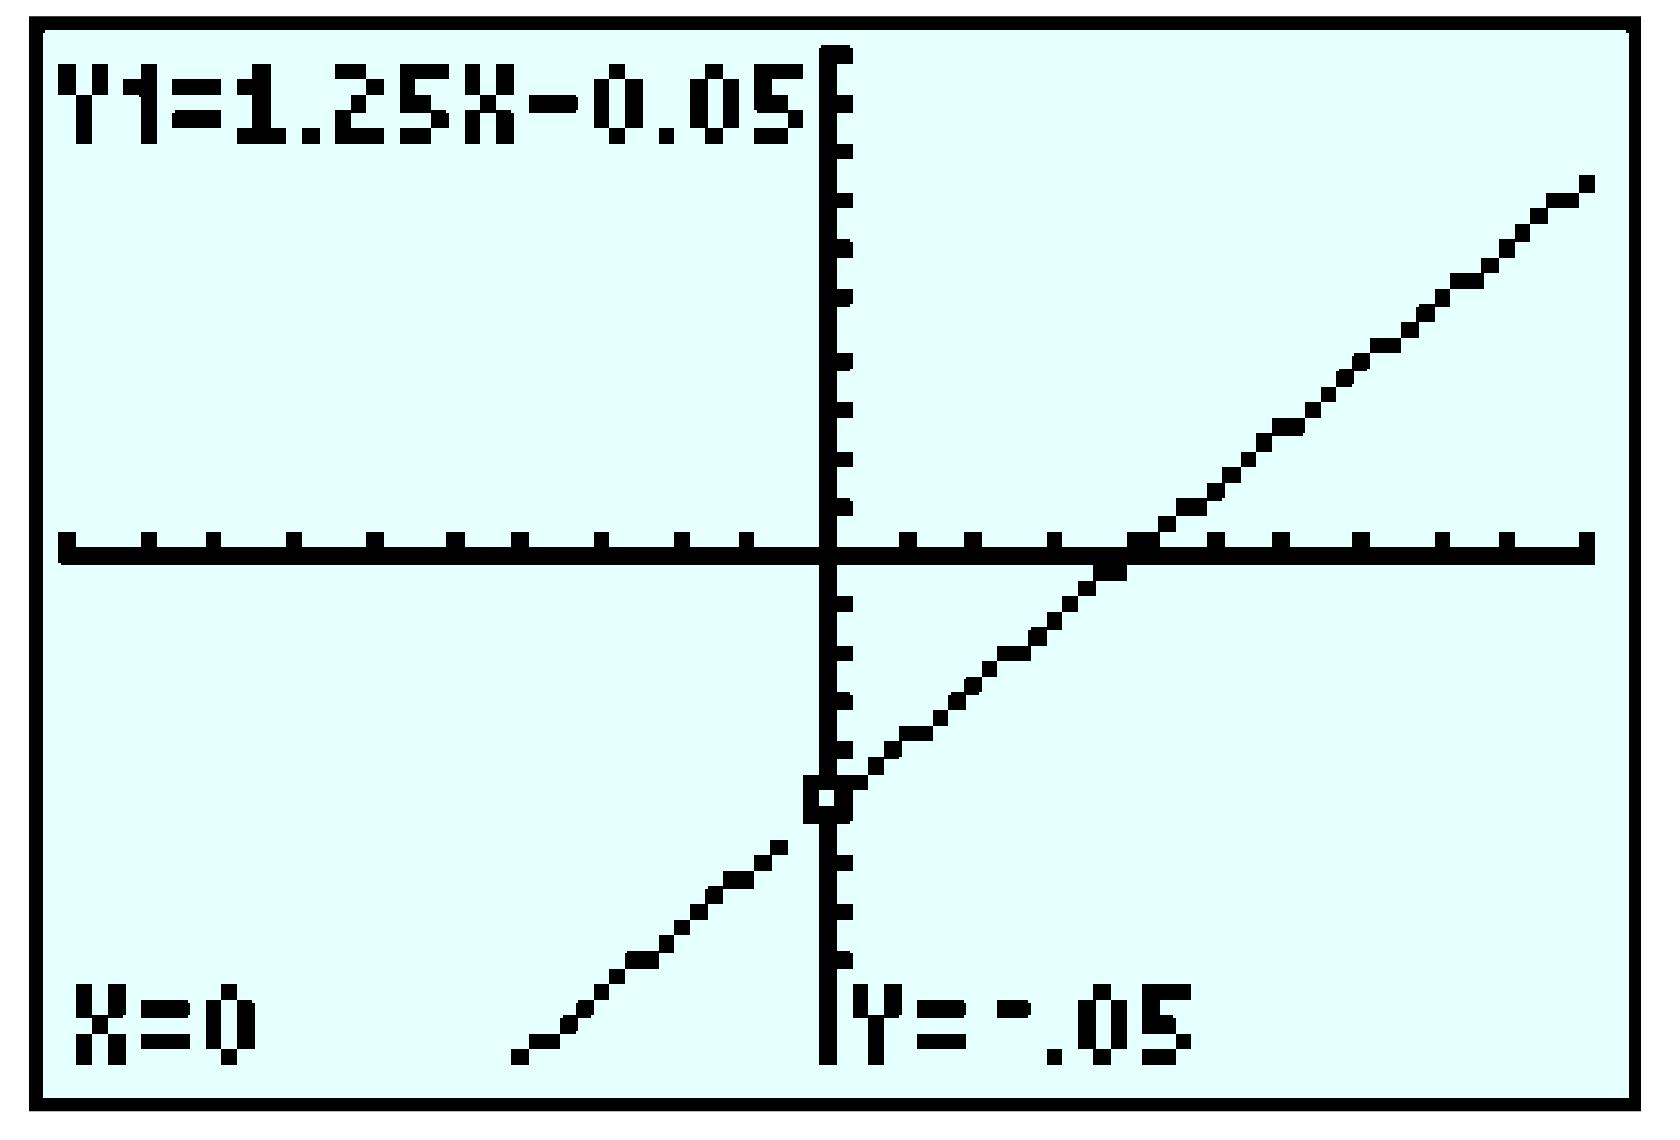
\includegraphics[width=0.5\linewidth]{images/fig-ans-1-1-47.jpg}
%
\end{enumerate}
%
\exercise[48.]\hypertarget{exercise-55}{}\(4x + 75y = 60,000\)%
\exercise[49.]\hypertarget{exercise-56}{}\(\dfrac{y}{12} - \dfrac{x}{60}= 1\)%
\par\smallskip
\noindent\textbf{Answer.}\hypertarget{answer-32}{}\quad
\leavevmode%
\begin{enumerate}[label=\alph*]
\item\hypertarget{li-244}{}\((-60, 0), (0, 12)\)%
\item\hypertarget{li-245}{}\(y = 12 + \dfrac{1}{5}x\)%
\item\hypertarget{li-246}{}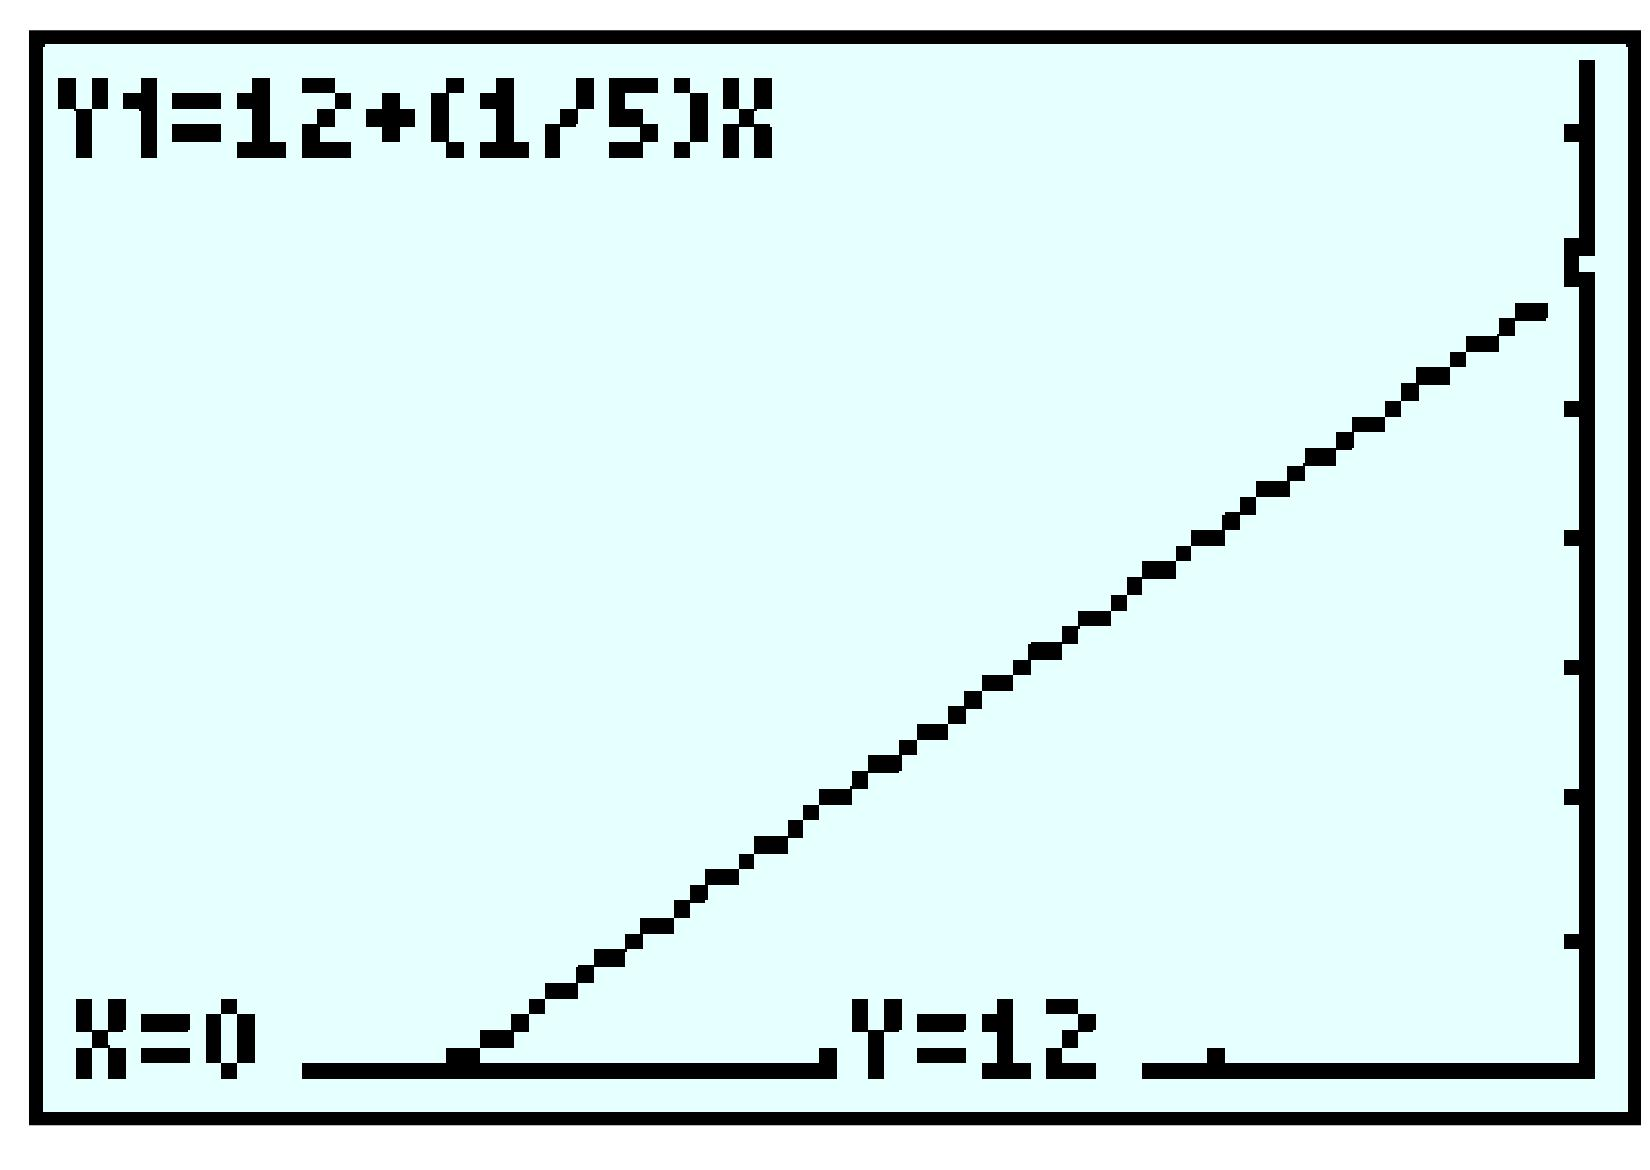
\includegraphics[width=0.5\linewidth]{images/fig-ans-1-1-49.jpg}
%
\end{enumerate}
%
\exercise[50.]\hypertarget{exercise-57}{}\(\dfrac{x}{80} + \dfrac{y}{400}= 1\)%
\exercise[51.]\hypertarget{exercise-58}{}\(-2x = 3y + 84\)%
\par\smallskip
\noindent\textbf{Answer.}\hypertarget{answer-33}{}\quad
\leavevmode%
\begin{enumerate}[label=\alph*]
\item\hypertarget{li-247}{}\((-42, 0), (0, -28)\)%
\item\hypertarget{li-248}{}\(y = \dfrac{-2}{3}x-28\)%
\item\hypertarget{li-249}{}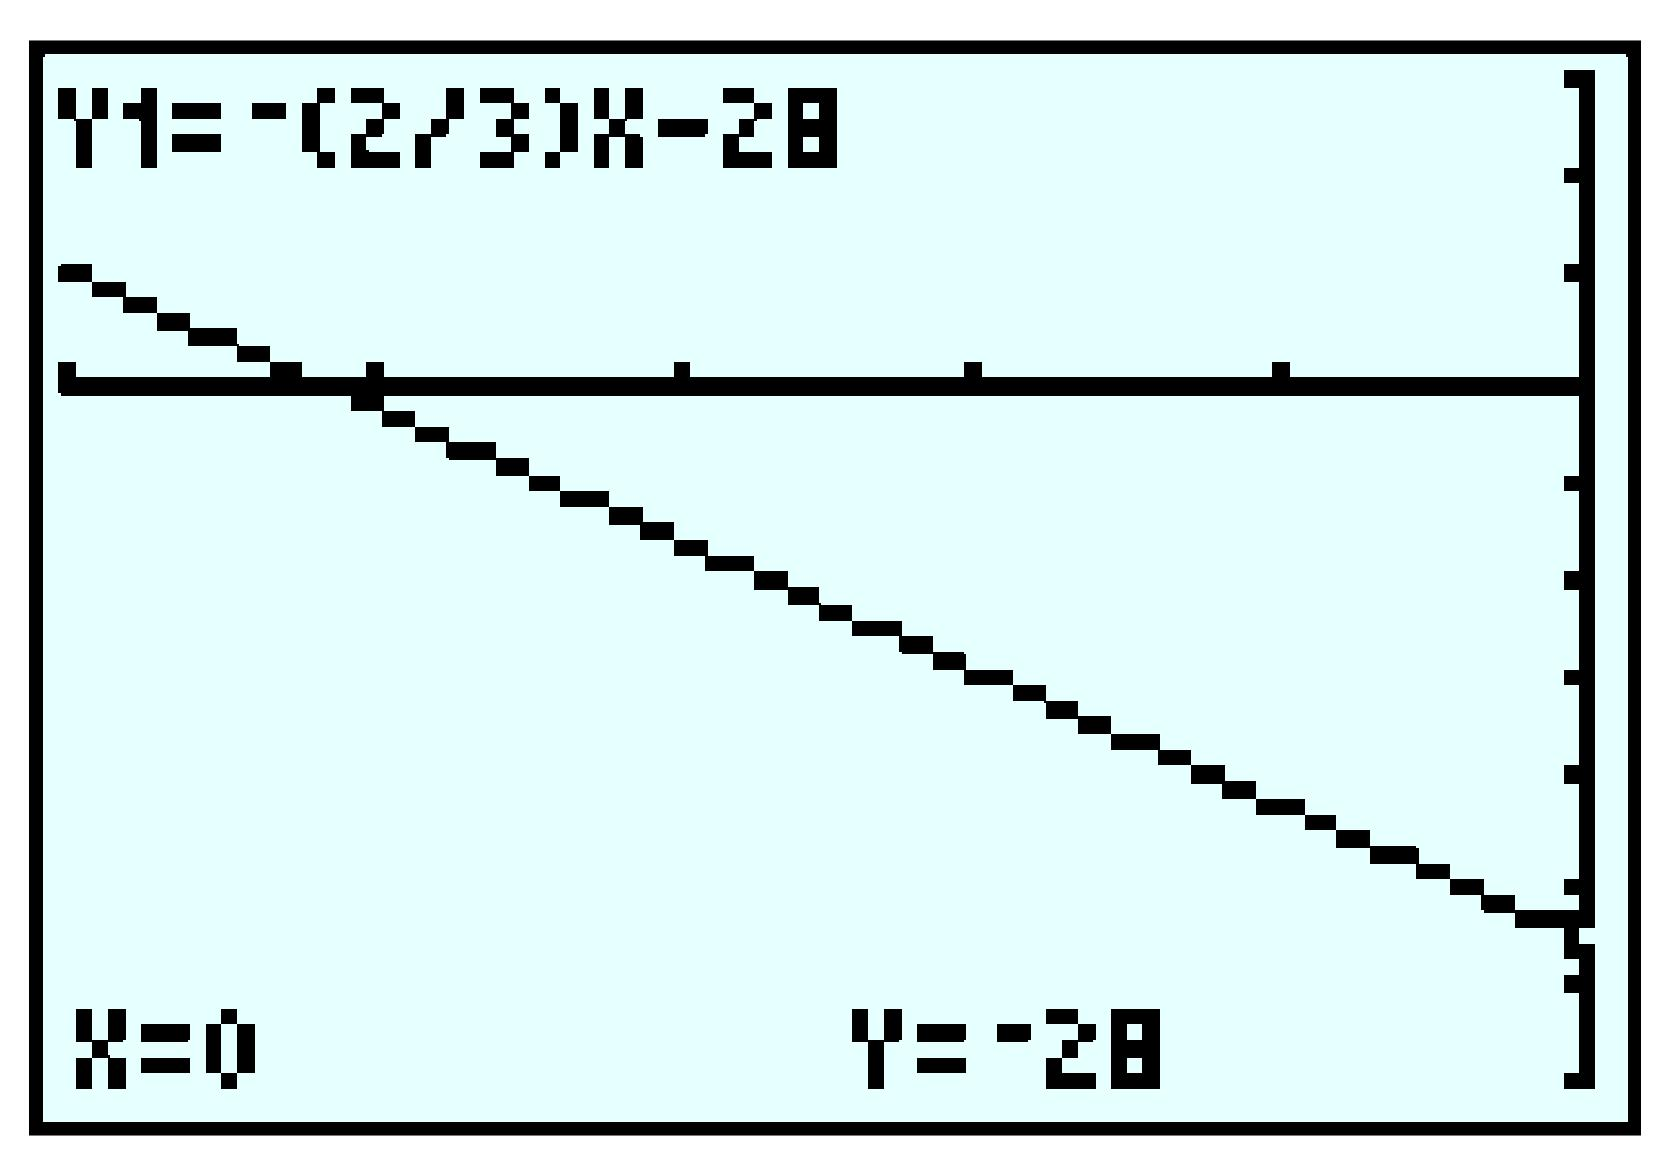
\includegraphics[width=0.5\linewidth]{images/fig-ans-1-1-51.jpg}
%
\end{enumerate}
%
\exercise[52.]\hypertarget{exercise-59}{}\(7x = 91 - 13y\)%
\end{exercisegroup}
\par\smallskip\noindent
\end{document}